\documentclass[10pt]{CSUNthesis}
%%%packages%%%
\usepackage[latin1]{inputenc}
%\usepackage{newcent}
\usepackage{verbatim}
\usepackage{graphicx}
\usepackage{amsmath}
\usepackage{amsfonts}
\usepackage{amssymb}
\usepackage{amsthm}
\usepackage[section]{placeins}
\usepackage{listings}%R Code
\usepackage{color}%R code
\usepackage{tikz}
\usetikzlibrary{patterns}
% \usepackage{tkz-graph}
% \usepackage{tkz-berge}
% \usepackage{tkz-euclide}
% \usepackage{hyperref}
%\usepackage[left=1in, right=1in, top=.9in, bottom=.9in]{geometry}
\usepackage{setspace}
%\usepackage{hyperref}
\usepackage{pdflscape}
\usepackage[english]{babel}
\usepackage{times}
\usepackage[T1]{fontenc}
\usepackage{multirow}
\usepackage{mathptmx}
%\usepackage[hidelinks]{hyperref}
\usepackage{lipsum}
\usepackage{titletoc}
\usepackage[toc,page]{appendix}
\usepackage{appendix}
\usepackage{enumerate}
\usepackage{enumitem}
%\usepackage{subfigure}
\usepackage{caption}
\usepackage{subcaption}
\usepackage{float}
%%CSUN Stuff%%%
\titlecontents{chapter}
  [0em]
   {\bfseries \addvspace{\baselineskip}}
  {\linebreak \rmfamily \chaptername\hspace{.1em} \thecontentslabel\quad \newline  }
  {\rmfamily}
  {\titlerule*[1pc]{.}\contentspage}

\titlecontents{section}
[1em]
   {}
  {\thecontentslabel \hspace{1em}}
   {}
    {\titlerule*[1pc]{.}\contentspage}

\titlecontents{subsection}
[3.3em]
   {}
  {\thecontentslabel \hspace{1.3em}}
   {}
    {\titlerule*[1pc]{.}\contentspage}

% for bibliography, abstract etc

\titlecontents{part}
  [0em]
   {\rmfamily \addvspace{\baselineskip}}
  {\linebreak \rmfamily \chaptername\hspace{.1em} \thecontentslabel\quad \newline  }
  {\rmfamily}
  {\titlerule*[1pc]{.}\contentspage}


\titlecontents{subsubsection}
[0em]
   {{\rmfamily \addvspace{\baselineskip}}}
  {\thecontentslabel \hspace{1em}}
   {}
    {\titlerule*[1pc]{}}
%%%END OF CSUN STUFF%%%
%%%theoerms, etc%%%%
\theoremstyle{plain}% default
\newtheorem{thm}{Theorem}[section]
\newtheorem{prop}{Proposition}[section]
\newtheorem{lem}{Lemma}[section]
\newtheorem{pf}{Proof}[section]
\theoremstyle{definition}
\newtheorem{definition}{Definition}[section]
\newtheorem{example}{Example}[section]
\theoremstyle{remark}
\newtheorem{rmk}{Remark}[section]
\newtheorem{case}{Case}
\newtheorem{prob}{Problem}[section]
%%%% R Code%%%%
\definecolor{dkgreen}{rgb}{0,0.6,0}
\definecolor{gray}{rgb}{0.5,0.5,0.5}
\definecolor{mauve}{rgb}{0.58,0,0.82}
\lstset{frame=tb,
  language=R,
  aboveskip=3mm,
  belowskip=3mm,
  showstringspaces=false,
  columns=flexible,
  basicstyle={\small\ttfamily},
  numbers=none,
  numberstyle=\tiny\color{gray},
  keywordstyle=\color{blue},
  commentstyle=\color{dkgreen},
  stringstyle=\color{mauve},
  breaklines=true,
  breakatwhitespace=true
  tabsize=3
}

%%%%%%%%TikZ Commands

\def\hexagonsize{1cm}
\pgfdeclarepatternformonly
  {hexagons}% name
  {\pgfpointorigin}% lower left
  {\pgfpoint{3*\hexagonsize}{0.866025*2*\hexagonsize}}%  upper right
  {\pgfpoint{3*\hexagonsize}{0.866025*2*\hexagonsize}}%  tile size
  {% shape description
   \pgfsetlinewidth{0.4pt}
   \pgftransformshift{\pgfpoint{0mm}{0.866025*\hexagonsize}}
   \pgfpathmoveto{\pgfpoint{0mm}{0mm}}
   \pgfpathlineto{\pgfpoint{0.5*\hexagonsize}{0mm}}
   \pgfpathlineto{\pgfpoint{\hexagonsize}{-0.866025*\hexagonsize}}
   \pgfpathlineto{\pgfpoint{2*\hexagonsize}{-0.866025*\hexagonsize}}
   \pgfpathlineto{\pgfpoint{2.5*\hexagonsize}{0mm}}
   \pgfpathlineto{\pgfpoint{3*\hexagonsize+0.2mm}{0mm}}
   \pgfpathmoveto{\pgfpoint{0.5*\hexagonsize}{0mm}}
   \pgfpathlineto{\pgfpoint{\hexagonsize}{0.866025*\hexagonsize}}
   \pgfpathlineto{\pgfpoint{2*\hexagonsize}{0.866025*\hexagonsize}}
   \pgfpathlineto{\pgfpoint{2.5*\hexagonsize}{0mm}}
   \pgfusepath{stroke}
  }
%%%%%%%%custom commands
\newcommand{\NN}{\mathbb{N}} %  set of natural numbers
\newcommand{\ZZ}{\mathbb{Z}} %  set of integer number
\newcommand{\RR}{\mathbb{R}} %  set of real numbers
\newcommand{\SH}{\mathbb{S}} %  set of unit vectors
\newcommand{\HH}{{\cal H}} %  Calligraphic H
\newcommand{\PP}{{\cal P}} %  Calligraphic P
\newcommand{\DD}{{\cal D}} %  Calligraphic D
\newcommand{\QQ}{{\cal Q}} %  Calligraphic D
\newcommand{\FF}{{\cal F}} %  Calligraphic D
\newcommand{\bbH}{{\mathbb{H}}}
\newcommand{\bbR}{{\mathbb{R}}}
\newcommand{\bbP}{{\mathbb{P}}}
\newcommand{\bbZ}{{\mathbb{Z}}}
\newcommand{\bbC}{{\mathbb{C}}}
\newcommand{\bbQ}{{\mathbb{Q}}}
\newcommand{\bbA}{{\mathbb{A}}}
\newcommand{\bbF}{{\mathbb{F}}}
\newcommand{\bbh}{{\mathbb{H}}}
\newcommand{\bbr}{{\mathbb{R}}}
\newcommand{\bbp}{{\mathbb{P}}}
\newcommand{\bbz}{{\mathbb{Z}}}
\newcommand{\bbc}{{\mathbb{C}}}
\newcommand{\bbq}{{\mathbb{Q}}}
\newcommand{\bba}{{\mathbb{A}}}
\newcommand{\bbf}{{\mathbb{F}}}
\newcommand{\bbn}{{\mathbb{N}}}
\newcommand{\bbN}{{\mathbb{N}}}
\newcommand{\disteq}{{\overset{D}{=}}}
\newcommand{\cross}{{\times}}
\newcommand{\CBeta}{{  \left( \begin{array}{c}\hat{\beta}_{1,1} - \hat{\beta}_{2,1} \\ \hat{\beta}_{1,2} -
\hat{\beta}_{2,2} \\ \vdots \\ \hat{\beta}_{1,p} - \hat{\beta}_{2,p}    \end{array} \right) }}
\newcommand{\COVW}{{\left[ \begin{array}{cc}\sigma_1^2 \left( X_1 ' X_1\right)^{-1}\\ \sigma_2^2 \left( X_2 '
X_2\right)^{-1} 
\end{array} \right]}}
\newcommand{\MSRES}{{\sigma_1^2 n_1 + \sigma_2^2 n_2 - p \left( \sigma_1^2 + \sigma_2^2 \right) }}
\newcommand{\XX}{{\left(X ' X\right)^{-1} }} 
\newcommand{\xx}{{\left(X ' X\right)^{-1} }} 
\newcommand{\ssres}{{\text{SS}_\text{RES}}}
\newcommand{\inv}[1]{{#1^{-1}}}
\renewcommand{\it}[1]{{\textit{#1}}}
% \newcommand{\iff}{{\Leftrightarrow}}
\newcommand{\comp}[2]{{\left( #1 \circ #2\right) }}
\newcommand{\set}[2]{{\left\lbrace \left.  #1 \left\vert #2  \right.\right.\right\rbrace  }}
\newcommand{\topo}{{\mathcal{T}}}
\newcommand{\powset}[1]{{\mathcal{P}\left( #1 \right) }}
%\newcommand{\vec}[1]{{\overrightarrow{#1} }}
%%%%Spacing commands %%%%%
\newcommand{\tab}{\hspace{.4cm}}
\newcommand{\quadtab}{\hspace{.4cm}}
\newcommand{\matab}{\hspace{1.01600mm}}
\renewcommand{\arraystretch}{1.5}
\newcommand{\RNum}[1]{\lowercase\expandafter{\romannumeral #1\relax}}
\newcommand{\rn}[1]{\lowercase\expandafter{(\romannumeral #1\relax)}}
\newcommand{\floor}[1]{\left\lfloor #1 \right\rfloor}
\newcommand{\ceil}[1]{\left\lceil #1 \right\rceil}
\newcommand{\combo}[2]{\left(\begin{array}{c}#1\\#2\end{array}\right)}
%\renewcommand{\baselinestretch}{1.0}
% 1.0 is for one line space, 2.0 is for double-line space, etc
%%%%Spacing commands %%%%%

%%%%Margins%%%%%% - Clinton Bowen
\setlength{\topmargin}{-.5in} 
\setlength{\textheight}{9.0in}
\setlength{\oddsidemargin}{0.5in} 
\setlength{\evensidemargin}{0.0in}
\setlength{\textwidth}{6.0in}
%%Please refer to http://en.wikibooks.org/wiki/LaTeX/Page_Layout
%%The parameters below are described pictorally on this webpage.  Tinker with the settins as needed.
%\setlength{\evensidemargin}{0cm}
%\setlength{\oddsidemargin}{0pt}
%\setlength{\topmargin}{.5in}
% \setlength{\hoffset}{0in}
% \setlength{\voffset}{0in}
% \setlength{\headheight}{0pt}
% \setlength{\headsep}{0in}%should be 1 inch from header titles
%\setlength{\textheight}{21cm}
%\setlength{\textwidth}{15.5cm}
% \setlength{\marginparsep}{0pt}
% \setlength{\marginparwidth}{0pt}
% \setlength{\footskip}{0pt}
%%%%Margins%%%%%% - Clinton Bowen
\author{Clinton Bowen}
\title{Protein Folding: Planar Configuration Spaces of Disc Arrangements and
Hinged Polygons: \textit{Protein Folding in Flatland}}
\date{April 1, 2014}
\makeindex
%CSUNthesis SETTINGS
\submitted{August}{2014}
\committee{Dr. Csaba T\'oth}{Dr. Silvia Fernandez}{Dr. John Dye}
\abstract{abstract goes here}
\begin{document}
\chapter{Background}

We consider four decision problems surrounding graph theory and geometry. 
The graph theory based problems involve polygonal linkages and the geometry based problems involve something called a contact graph of disks.  
In each problem, we decide whether a polygonal linkage or contact graph has a certain realization in the plane.

This thesis first presents preliminary information needed to pose our four problems, then we formally pose each problem and then provide the hardness results in all four cases.
We show that all four problems are intractable, or $\NP$ hard (see definition below). 

\section{Graphs}
A \textit{graph} is an 
ordered pair $G = (V,E)$ comprising of a set $V$ of vertices and a set $E$ of edges or 
lines.  Every edge $e \in E$, is an unordered pair of distinct vertices $u,v \in V$ (
the edge represents their adjacency, $e = \{ u,v\}$). With this definition of a graph, there 
are 
no loops (self adjacent vertices, $\{v,v\}$) or multi-edges (several edges between the same pair of 
vertices).

A motivation for using graphs is modelling physical objects like molecules.  This requires an 
embedding into the plane or $\bbr^3$.  An \textit{embedding} of the 
graph $G = (V,E)$ is an injective mapping $\Pi : V \mapsto \bbR^{2}$ (see Figure 
\ref{fig:graph1-1}). 

\begin{figure}[!htbp]
\begin{center}
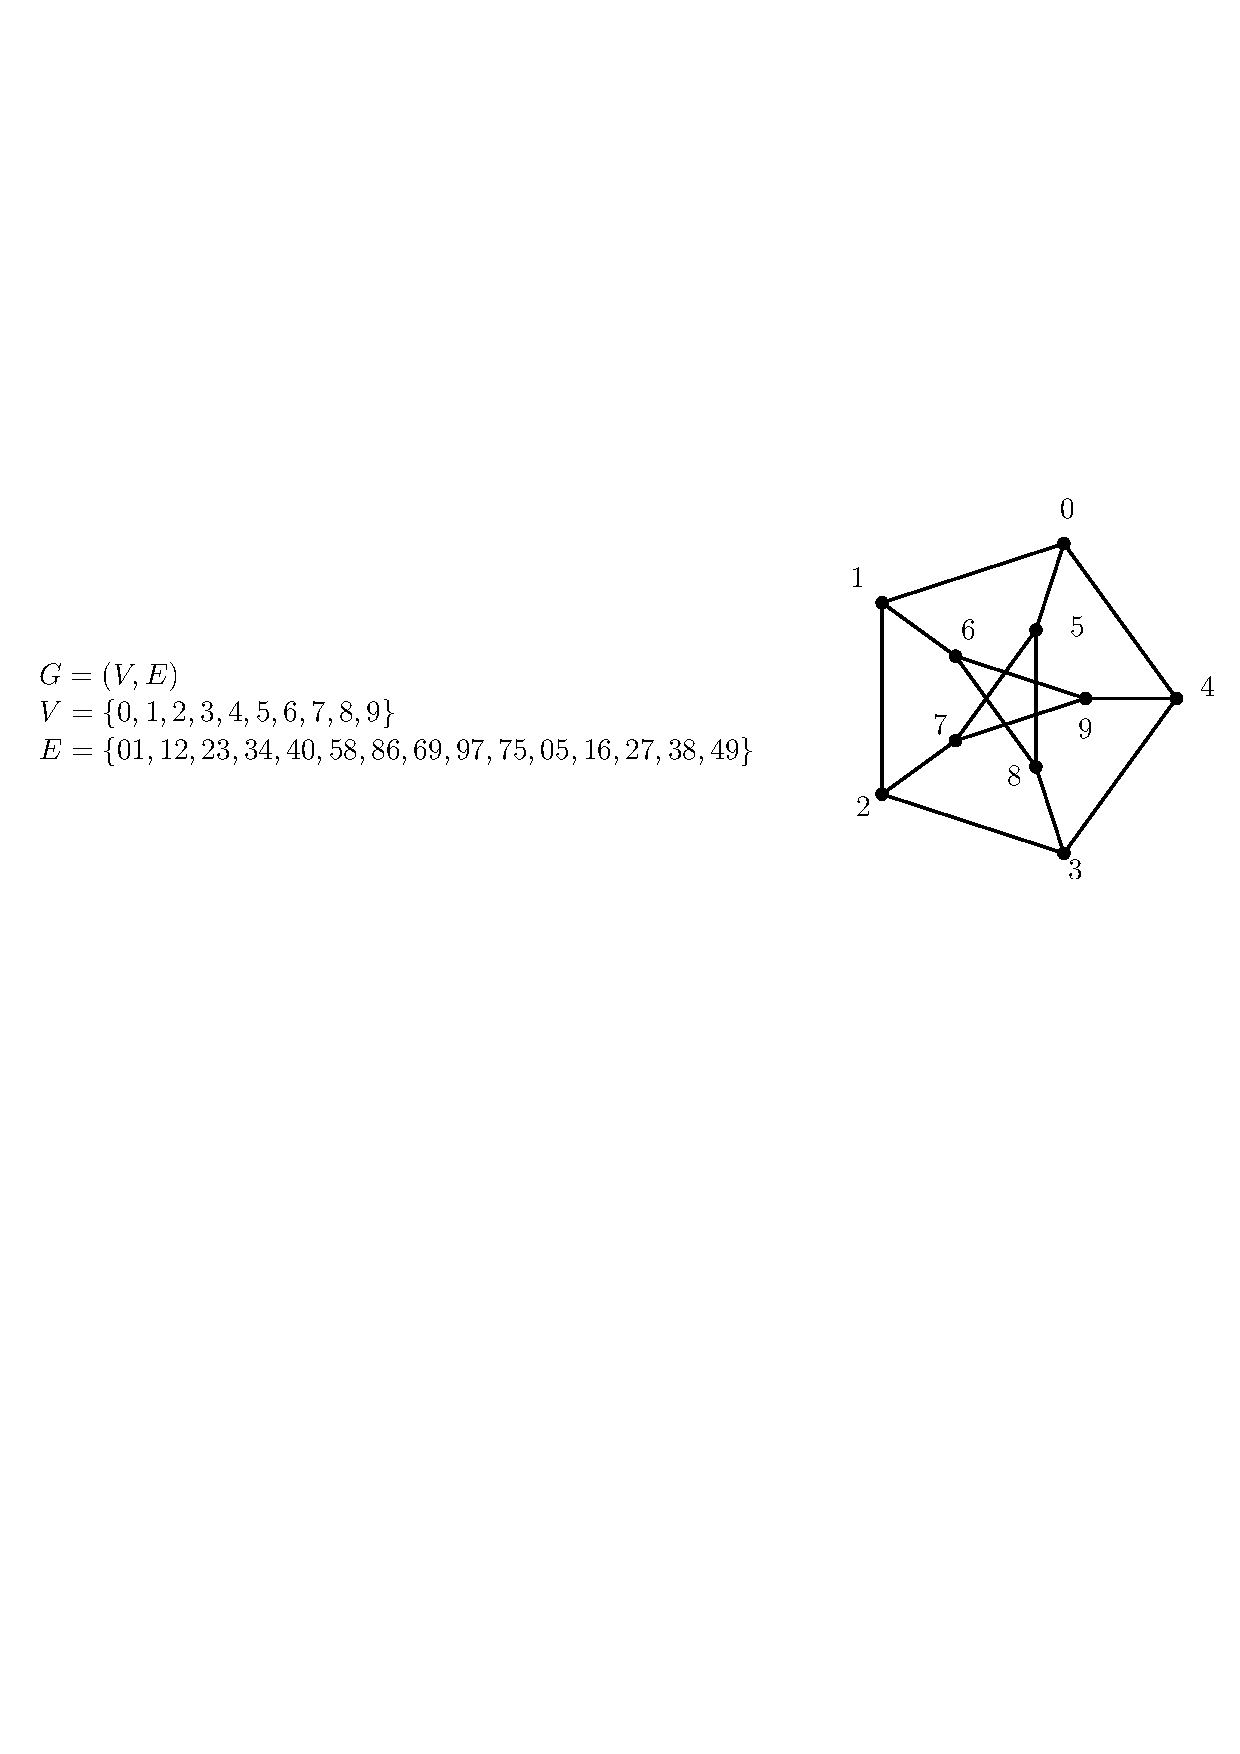
\includegraphics[scale=.5]{graphics/PetersonGraphExample.pdf}
\caption{An embedding of the Peterson graph.}\label{fig:graph1-1}
\end{center} 
\end{figure} 
\subsubsection{Edge Crossings}
We define \textit{plane embeddings} of a graph to be an embedding where the following degenerate 
configurations 
do not occur:
\begin{itemize}
\item[\rn{1}] the interiors of two or more edges intersect, or
\item[\rn{2}] an edge passes through a vertex
\end{itemize} 
\begin{figure}[H]
\begin{center}
  \begin{subfigure}[b]{0.49\textwidth}
	  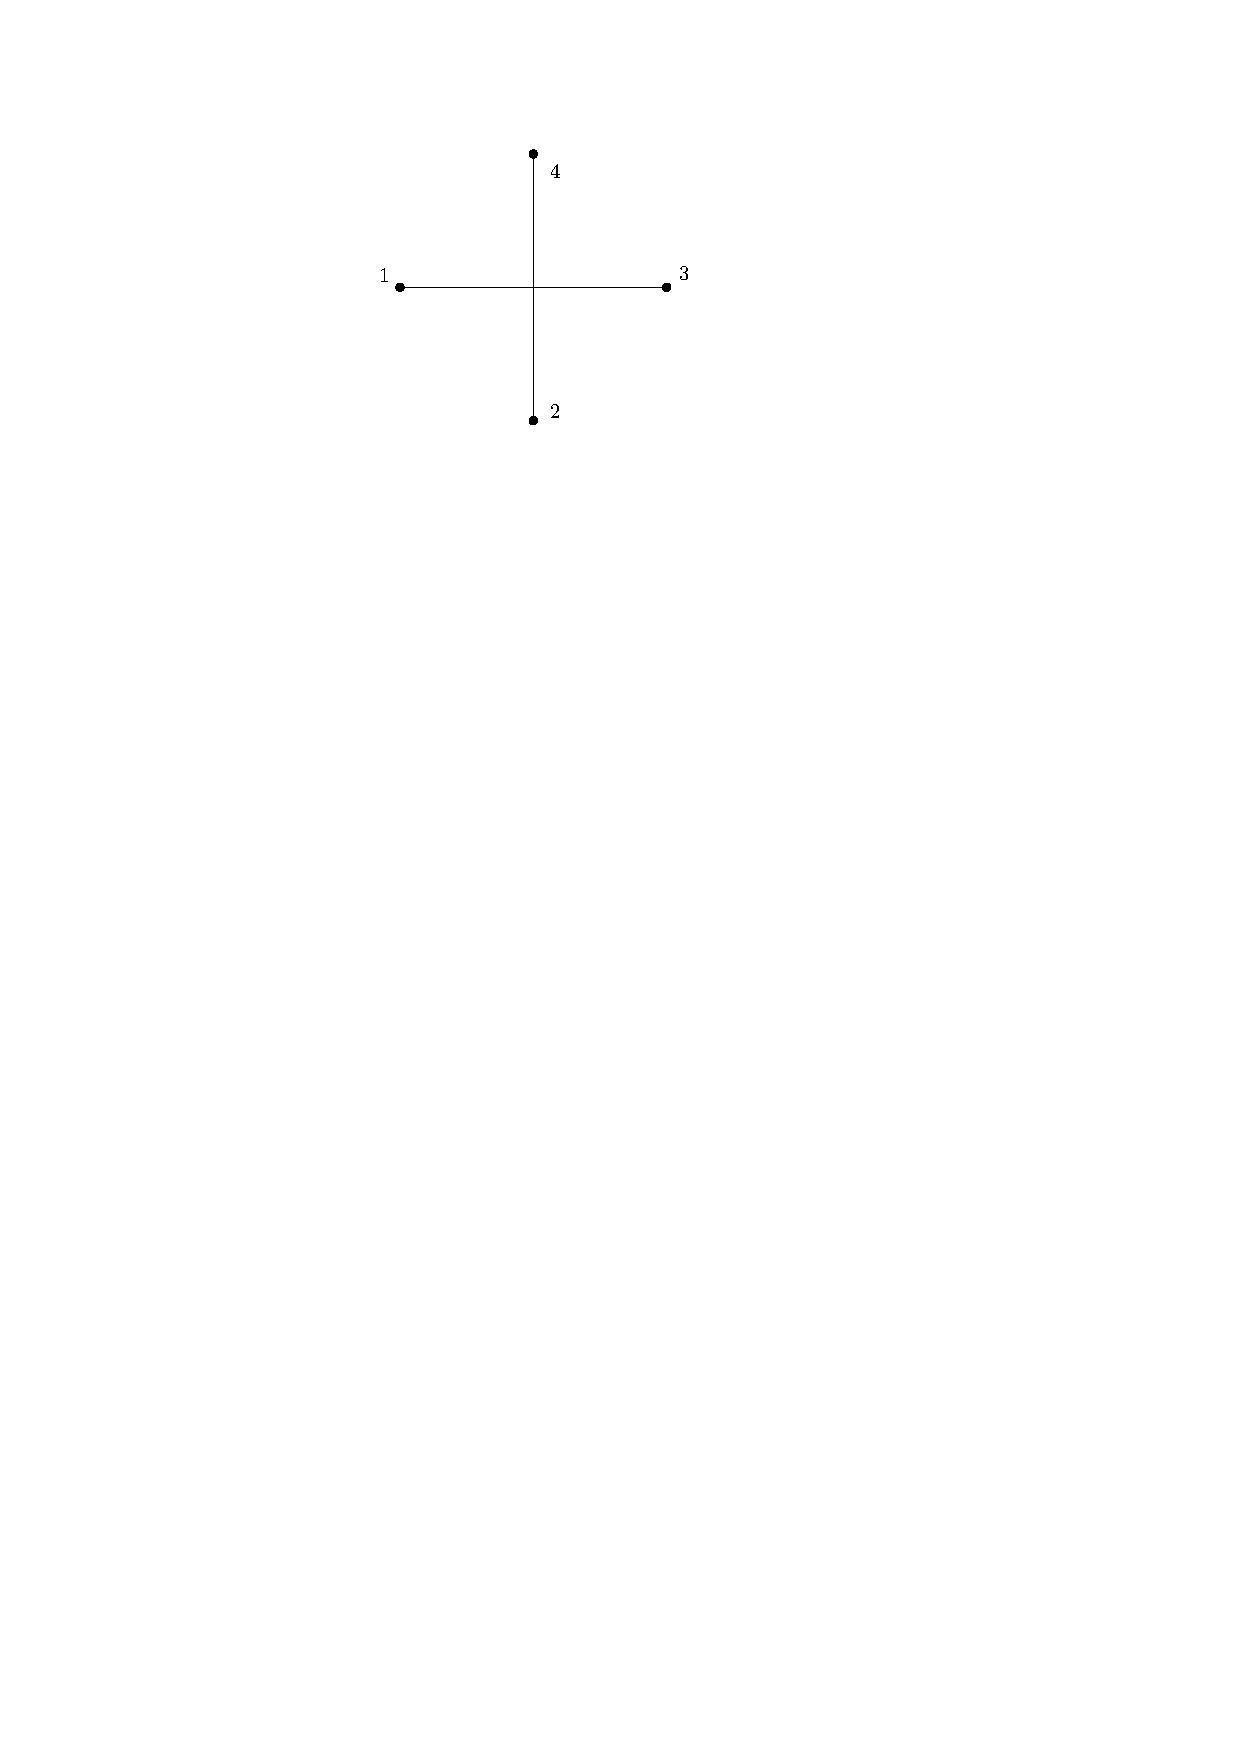
\includegraphics{graphics/crossingType2.pdf}
	  \caption{The interior of the edges intersect.}
	  \label{fig:ch1-linkages-1-2}
  \end{subfigure}
  \begin{subfigure}[b]{0.49\textwidth}
	  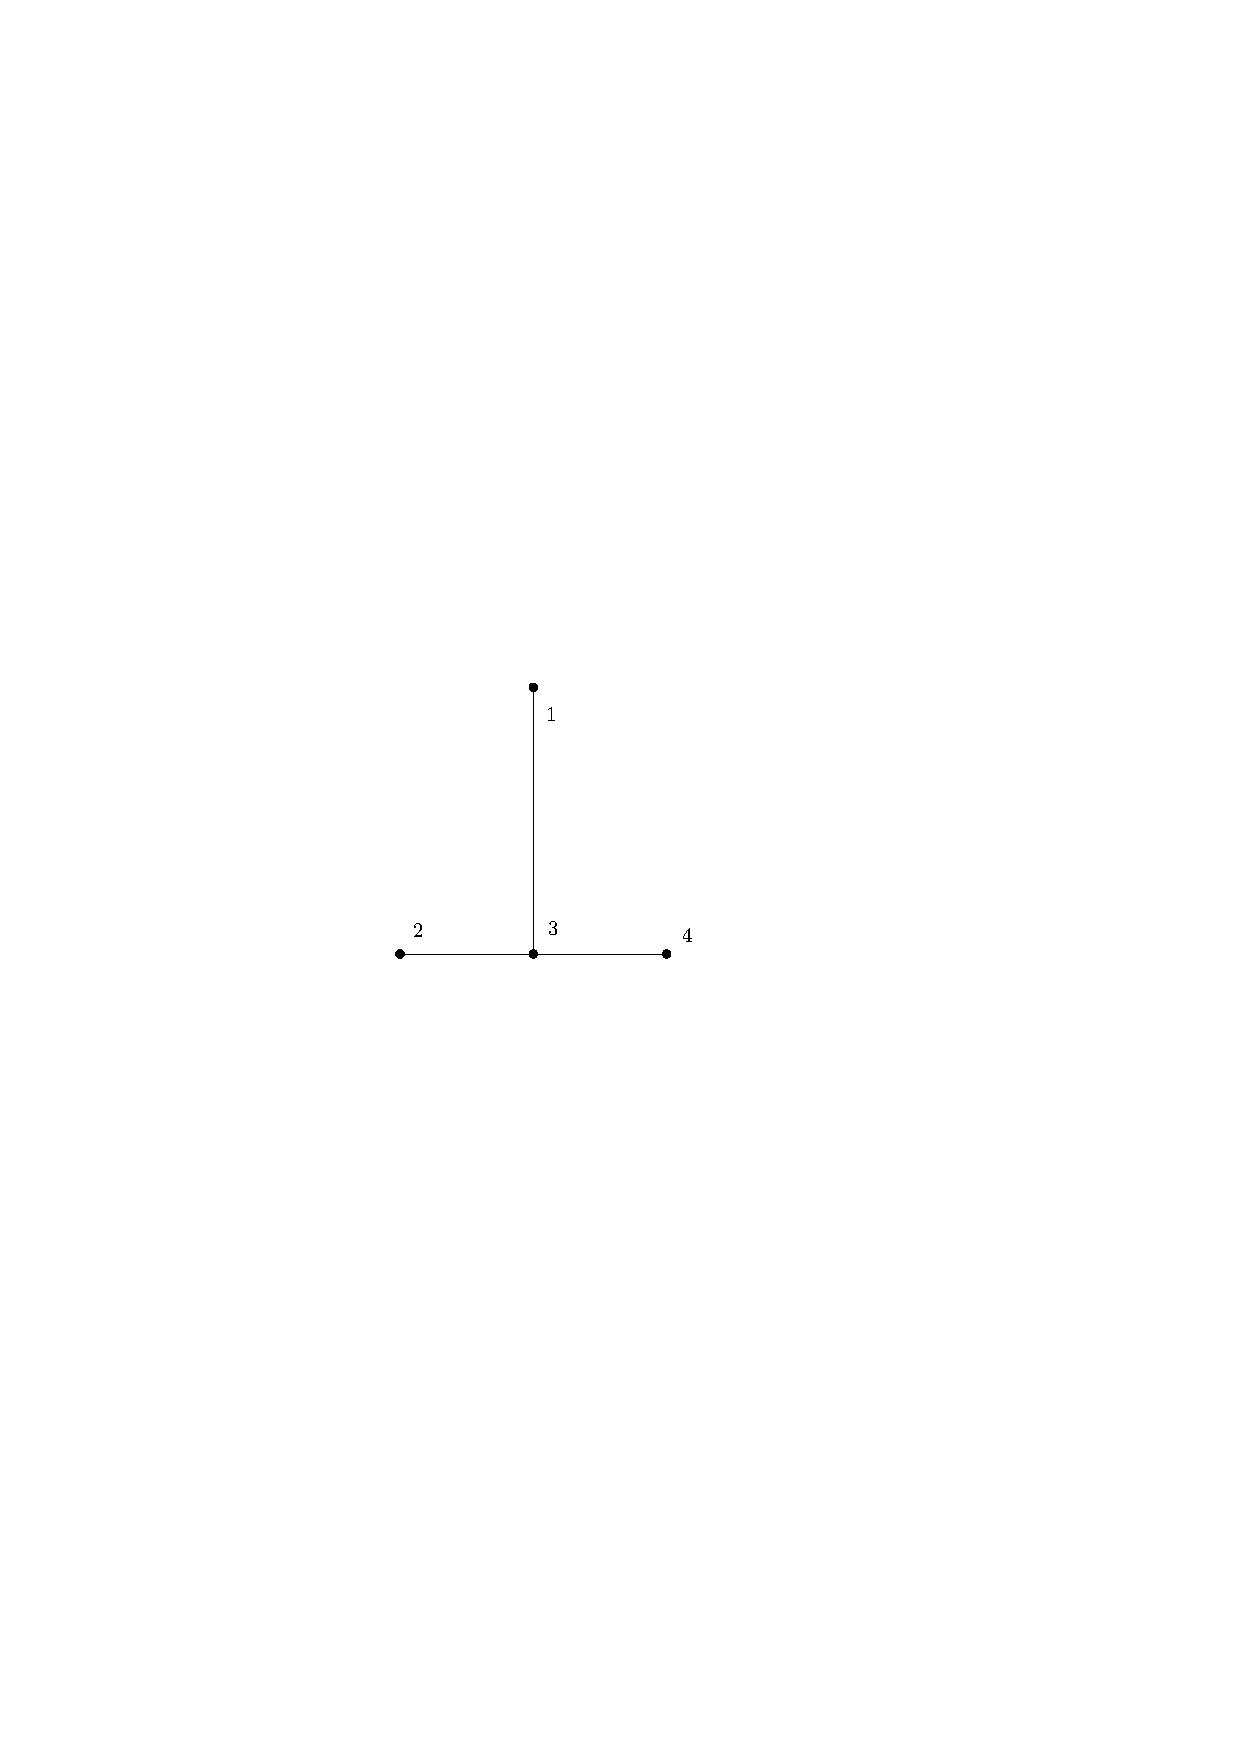
\includegraphics{graphics/crossingType3.pdf}
	  \caption{An edge passes through a vertex.}
	  \label{fig:ch1-linkages-1-3}
  \end{subfigure}
\end{center} 
\caption{These figures exhibit the 4 types of edge crossings.}\label{fig:ch1-linkages-1}
\end{figure}
A graph is called \textit{planar} if it admits a plane embedding.  A \textit{plane graph} is a 
graph together with a plane embedding.
\subsection{Trees}
A \textit{path} is a sequence of vertices in which every two consecutive vertices are connected by 
an edge.   
A \textit{simple  cycle} of a graph is a sequence, $(v_1, v_2, \dots, v_{t-1},v_t)$, of 
distinct vertices such that every two consecutive vertices are connected by 
an edge,  and the last vertex, $v_t$, connects to $v_1$.  A 
graph is \textit{connected} if for any two vertices, there exists a path between 
the two points.

A \textit{tree} is a graph that has no simple cycles and is connected.
\begin{figure}[h]
\begin{center}
  \begin{subfigure}[b]{0.49\textwidth}
    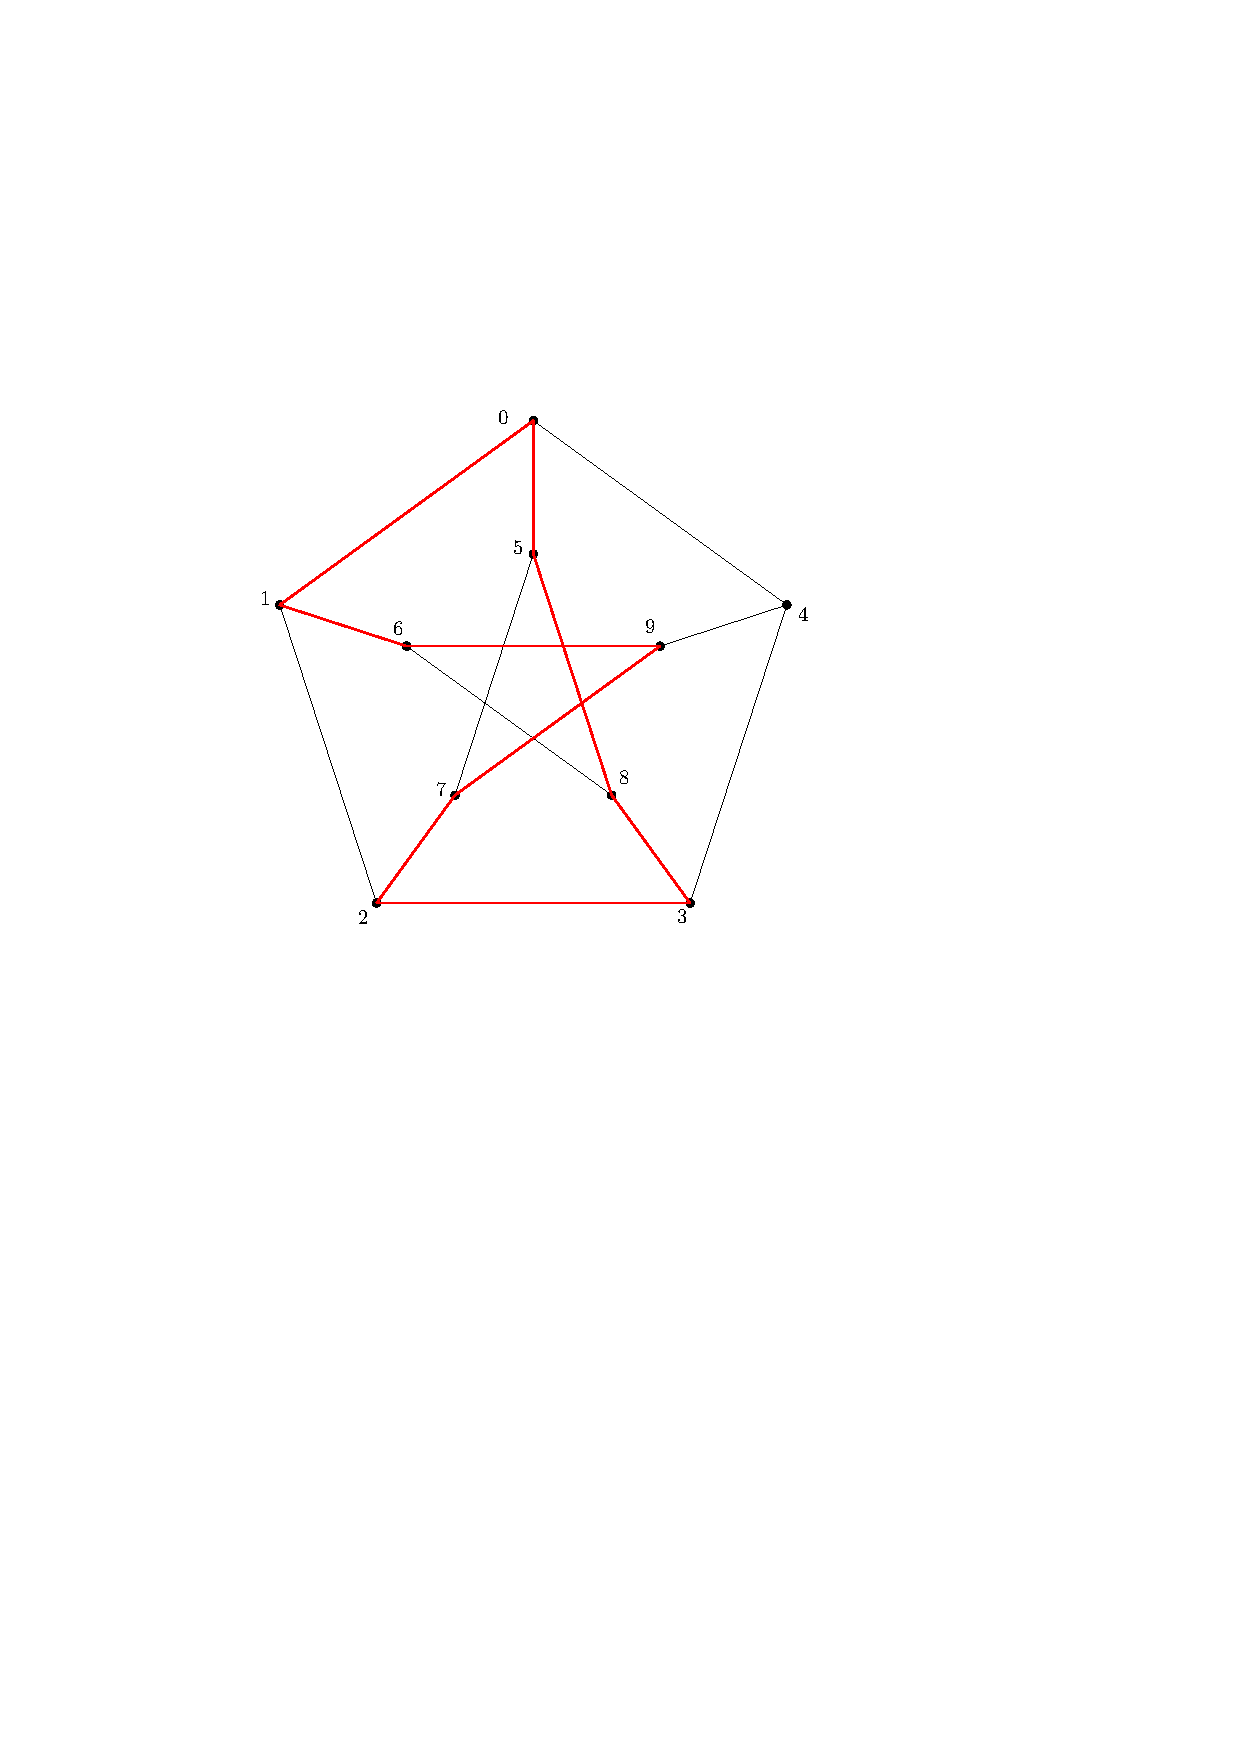
\includegraphics{graphics/PetersonGraphAgain.pdf}
    \caption{An embedding of the Peterson graph with a simple cycle of 
    (2,7,9,6,1,0,5,8,3).}\label{fig:ch1-graph-2}
  \end{subfigure}
  
\end{center}
\end{figure}
\subsection{Ordered Trees}
An \textit{ordered tree} is a tree together with a cyclic order of the neighbors for each vertex.
\begin{figure}[h]
\begin{center}
    \includegraphics{graphics/OrderedTreesExample.pdf}
    \caption{A tree with two embeddings with different cyclic orderings around 
vertices.}\label{fig:ch1-graph-6}
\end{center}
\end{figure}
Embeddings of ordered trees are equivalent if for each node the counter-clockwise ordering of 
adjacent nodes are the same.
\subsection{Graph Isomorphism} 
To determine when two graphs are equivalent, we need to define an isomorphism for graphs.  Given 
two graphs $G_1 =(V_1,E_1)$ and $G_2 = (V_2,E_2) $, a \textit{graph isomorphism} a bijective 
function $f: V_1 \mapsto 
V_2$ 
such that for any two vertices $u,v \in V_1$, we have $\{u, v\} \in E_1$, if and 
only 
if $(f(u),f(v)) \in E_2$. 
\begin{table}[!ht]
\begin{center}
$$\begin{array}{|c|c|c|}\hline
\text{Graph}&\text{Vertices}&\text{Edges}\\\hline
G_1&\left\lbrace a,b,c,d,e \right\rbrace & \left\lbrace ab,(b,c),(c,d),(d,e),(e,a) \right\rbrace 
\\\hline
G_2&\left\lbrace 1,2,3,4,5 \right\rbrace & \left\lbrace (1,2),(2,3),(3,4),(4,5),(5,1) \right\rbrace 
\\\hline
\end{array} $$
\caption{Two graphs that are isomorphic with the alphabetical isomorphism $f(a)=1$, $f(b)=2$, $f(c) 
= 3$, $f(d)=4$, $f(e)=5$.}
\end{center} 
\label{table:ch1-graph-1}
\end{table}

\begin{figure}[!h]
\begin{center}
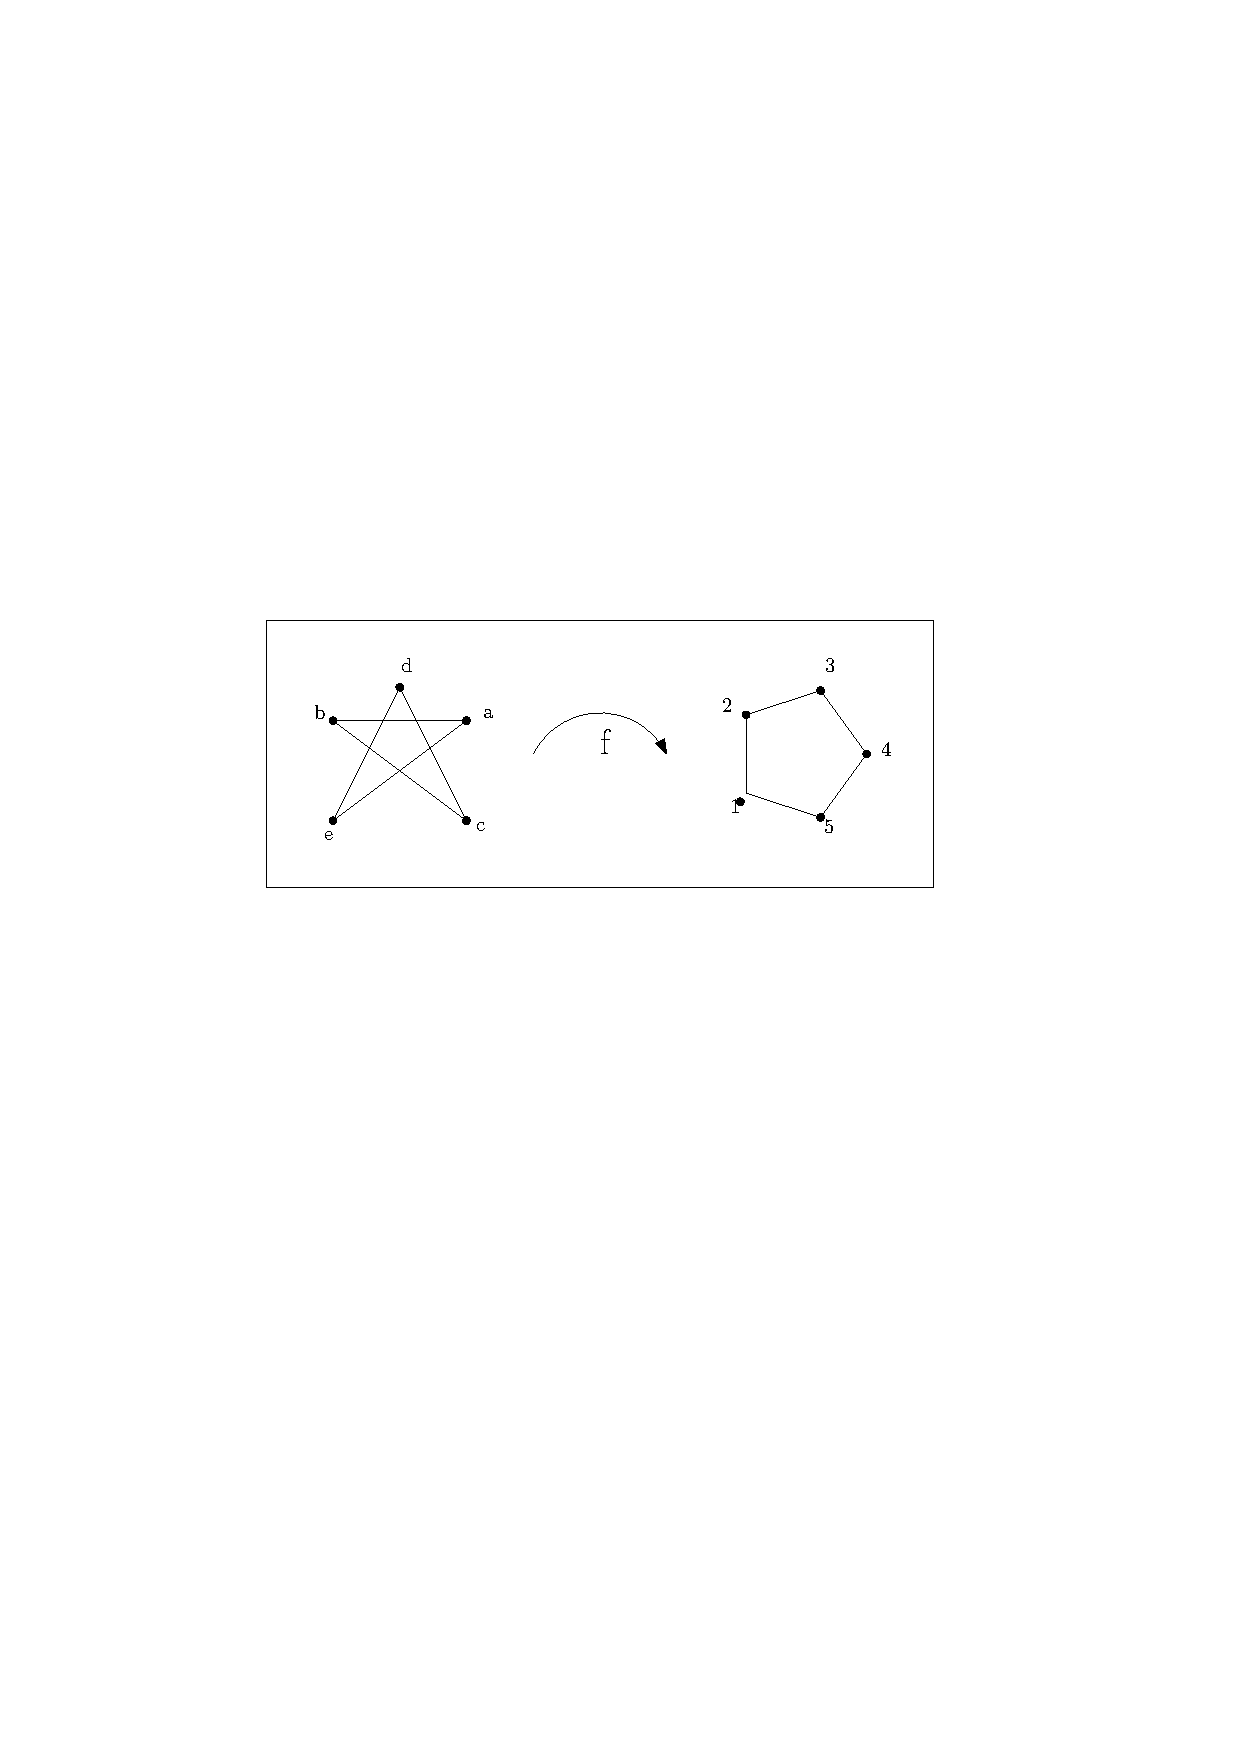
\includegraphics[scale=1]{graphics/graphIsomorphismExample.pdf}
\end{center} 
\caption{This figure depicts the graph isomorphism shown in Table 
(\ref{table:ch1-graph-1}) between 
$V_1$ and $V_2$ in the plane.}
\label{fig:configuration-3}
\end{figure}


% Next we add restrictions to our graph isomorphisms to narrow our focus:
% \begin{itemize}
% \item[\rn{1}] We focus on isomorphisms for planar graphs and or polygonal linkages, simple planar 
% graphs, and
% \item[\rn{2}] the isomorphism preserves edge lengths (polygonal area), e.g. $d(u,v) = d(f(u),f(v))$.
% \end{itemize}  
% With these restrictions of our isomorphisms, we can begin to describe a range of motion to 
% transform a linkage.  That range of motion is said to be the configuration space of that linkage.  
% To expand on this concept, for given linkage, $L=(V,E)$, and for a given vertex $v \in V$, the set 
% of points in which $v$ can be realized in the plane would be the configuration space for that 
% vertex, $C_v$.  Defining some order of the vertices in $L$, i.e. $V = \left\lbrace v_n 
% \right\rbrace_{i=1}^n$, then the \it{configuration space} for $L$ is said to be the cartesion 
% product of the configuration space of vertices:
% \subsection{Summary}
% \begin{table}[!ht]
% \begin{center}
% $$\begin{array}{|l|c|c|}
%  \hline
% &\text{Linkages}&\text{Polygonal Linkages}\\\hline
% \text{Ordered Pair}&G&G\\\hline
% \text{Edges}&E&\HH\\\hline
% \text{Vertices}&V&\PP\\\hline
% l&l&\text{N.A.}\\\hline
% \text{Embedding of }G&\Pi : V \mapsto \bbr^2&\PP ' = \left\lbrace P_i ' 
% \right\rbrace_{i=1}^n\\\hline
% \text{Realization}&\text{See (a)}&\text{See (b)}\\\hline
% \end{array}
% \caption
% $$
% \caption{(a)The realization for a linkage is for any edge $(u,v) \in E$ such that $\left\vert 
% \Pi(u)-\Pi(v)\right\vert = l(u,v)$.(b)A \emph{realization} of a polygonal linkage is an 
% interior-disjoint placement of congruent copies of the polygons in $\PP$ such that the points 
% corresponding to each hinge are identified (Fig. \ref{fig:1}, left).(c).}
% \end{center} 
% \label{table:linkages-2}
% \end{table} 
% %1) 
% %DESCRIBE THE FOLLOWING:
% %1)CONFIGURATION SPACE AS A VECTOR SPACE OF DIMENSION 2^N WHERE EDGE LENGTH IS PRESERVED.
% %2)PINNING 1 VERTEX TO ORIGIN AND A NEIGHBOR, ADD MOTIVATION TO PREVENT ROTATION AND TRANSLATIONS.
% 
% % \begin{equation}\label{eqn:linkages-1}
% % C(L) = C_{v_1} \cross C_{v_2} \cross \cdots \cross C_{v_n}
% % \end{equation} 
% % Some food for thought on configuration spaces and motions on linkages:
% % \begin{itemize}
% % \item[\rn{1}] A configuration space is said to be \it{connected} if there is a continuous mapping 
% for any two planar realizations (linkages) of a graph in the plane.  Otherwise it is said to be 
% \it{disconnected}.
% % \item[\rn{2}] If the configuration space of a vertex, $C_v$, is a singleton set, then the vertex 
% is said to be \it{pinned}. Otherwise it is said to be \it{free}.
% % \item[\rn{3}] The types of motions (mappings) that we refrain from using on linkages are 
% translations.
% % \end{itemize}
% % Note that configuration spaces for polygonal linkages are described similarly.
% % \subsubsection{Realizability of Linkages}
% % Suppose we had two configurations of a linkage, $\mathcal{A}$ and $\mathcal{B}$.  A question that 
% can be posed is can we reconfigure $\mathcal{A}$ to $\mathcal{B}$ continuously while respecting 
% simple planar graph conditions?  The answer to this question is a yes or no.  If yes, then there 
% must exist a path connected configuration space between $\mathcal{A}$ and $\mathcal{B}$.  It has 
% been shown that this problem can be posed as a planar satisfiability problem 
% \cite{Breu19983,mulzer2008minimum} (Later on in this paper we'll cover satisfiability problems).  
% This is the type of problem that we face in this paper.  We will continue to explore this in a 
% different manner, with circle packings.
% \newpage 

\subsection{Linkages}
\begin{definition}[Graph]\label{def:linkages-2}
An ordered pair $G = (V, E)$ comprising a set $V$ of vertices or nodes together with a set $E$ of edges or lines
\end{definition} 
\begin{definition}[Linkage]\label{def:linkages-1}
A collection of fixed-length 1D segments joined at their endpoints to form a graph.
\end{definition} 
A linkage can be thought of as a type of path-connected graph, i.e. the segments of a linkage are the edges of a graph, and the endpoints of the segments are the vertices.
\begin{definition}[Cycle]\label{def:linkages-3}
 A closed walk with no repetitions of vertices or edges allowed, other than the repetition of the starting and ending vertex
\end{definition} 
\begin{definition}[Configuration]\label{def:linkages-6}
A specification of the location of all the link endpoints, link orientations and
joint angles.\cite{demaine2008geometric}
\end{definition}
\begin{definition}[Configuration Space]\label{def:linkages-7}
The space of all configurations of a linkage.
\end{definition} 
A configurations space is said to be continuous if for any two configurations, $\mathcal{A}$ and $\mathcal{B}$ of a linkage $L$, $\mathcal{A}$ can be continuously reconfigured to $\mathcal{B}$ such that, the reconfigurations reside in the configuration domain, $L$ remains rigid throughout reconfiguration (i.e. all links' lengths are preserved), and no violations of linkage intersection conditions. 
\begin{definition}[Pinned Joint]\label{def:linkages-8}
A vertex of a graph (or linkage) that is fixed to a position in a plane.
\end{definition} 
\begin{definition}[Free Joint]\label{def:linkages-8}
A vertex of a graph (or linkage) that is not fixed to a position in a plane.
\end{definition} 
\begin{figure}[h]
\begin{center}
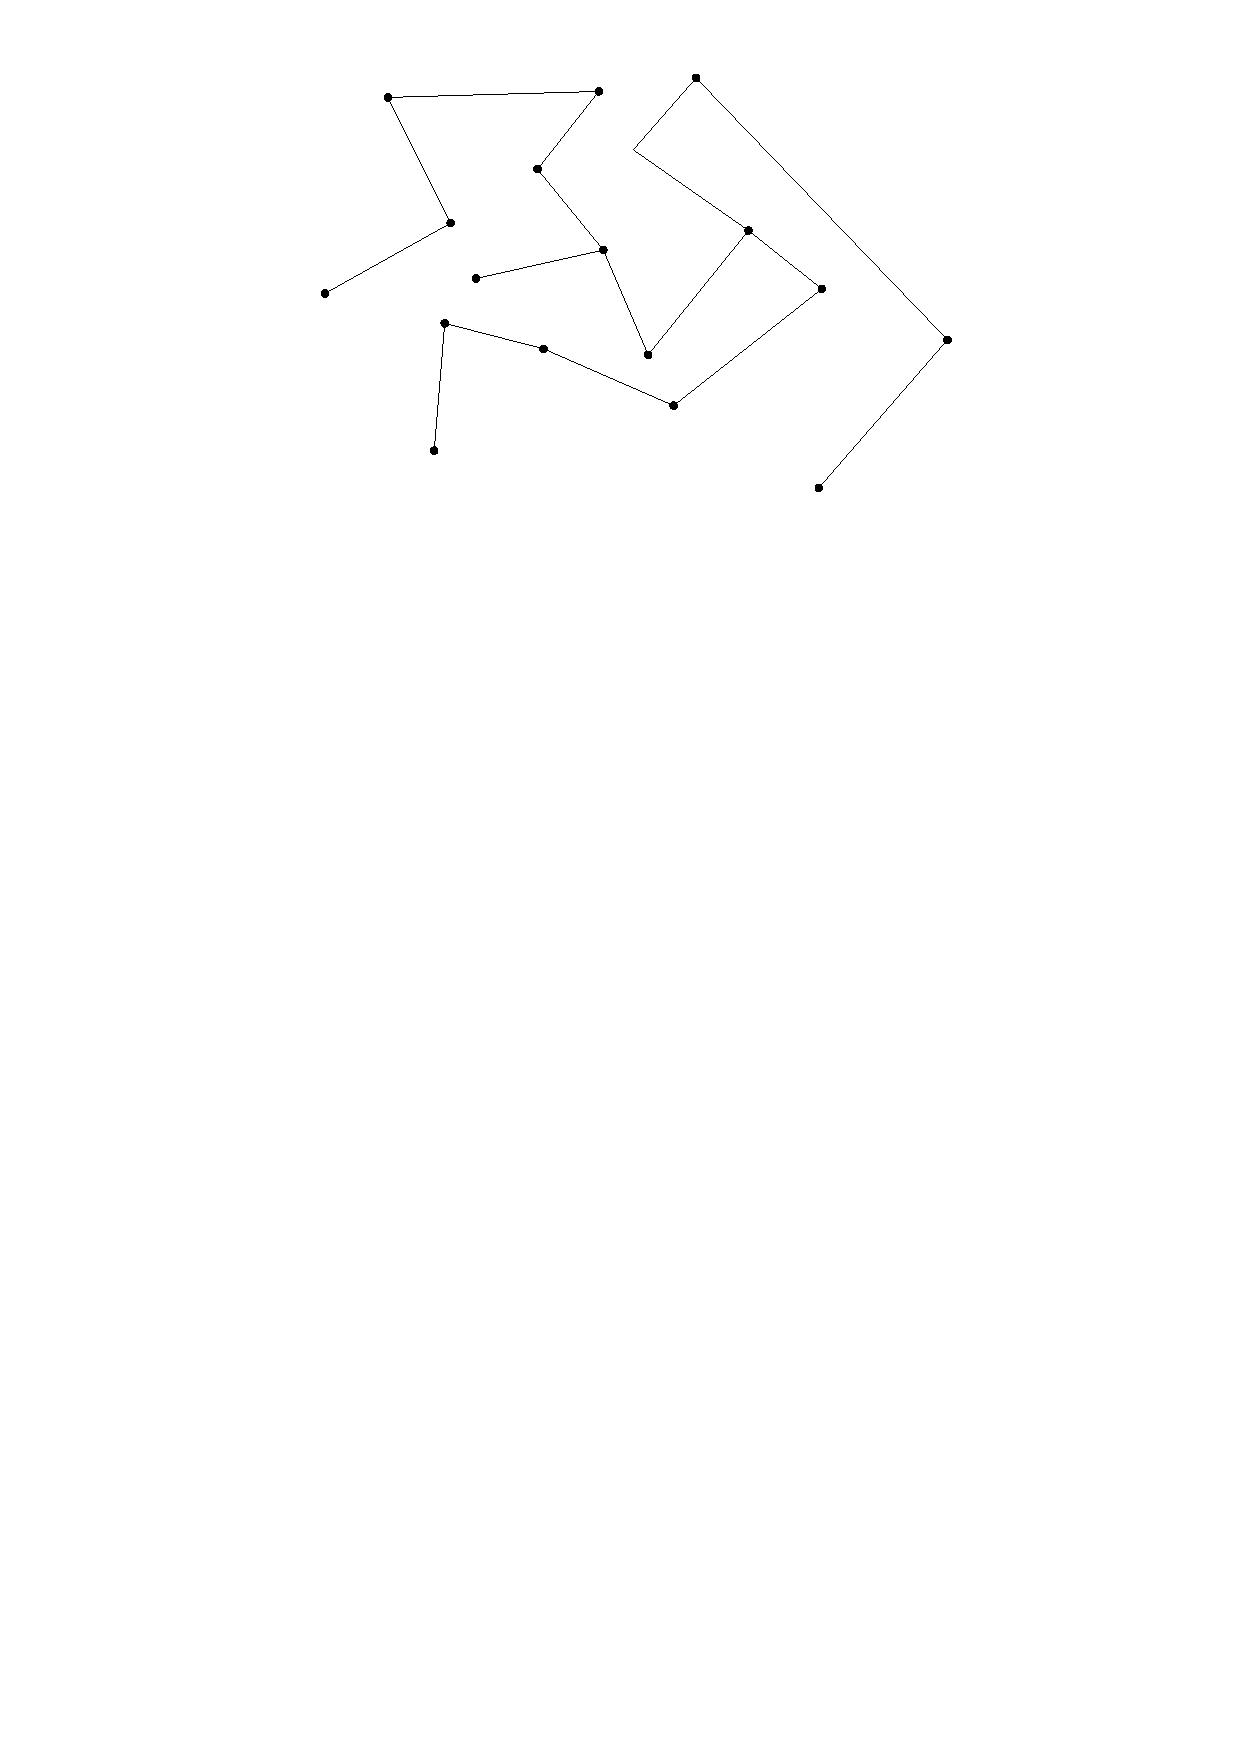
\includegraphics[scale=.5]{graphics/randomLinkage.pdf}
\end{center} 
\caption{A linkage with joints.}
\end{figure} 
\begin{figure}[h]
\begin{center}
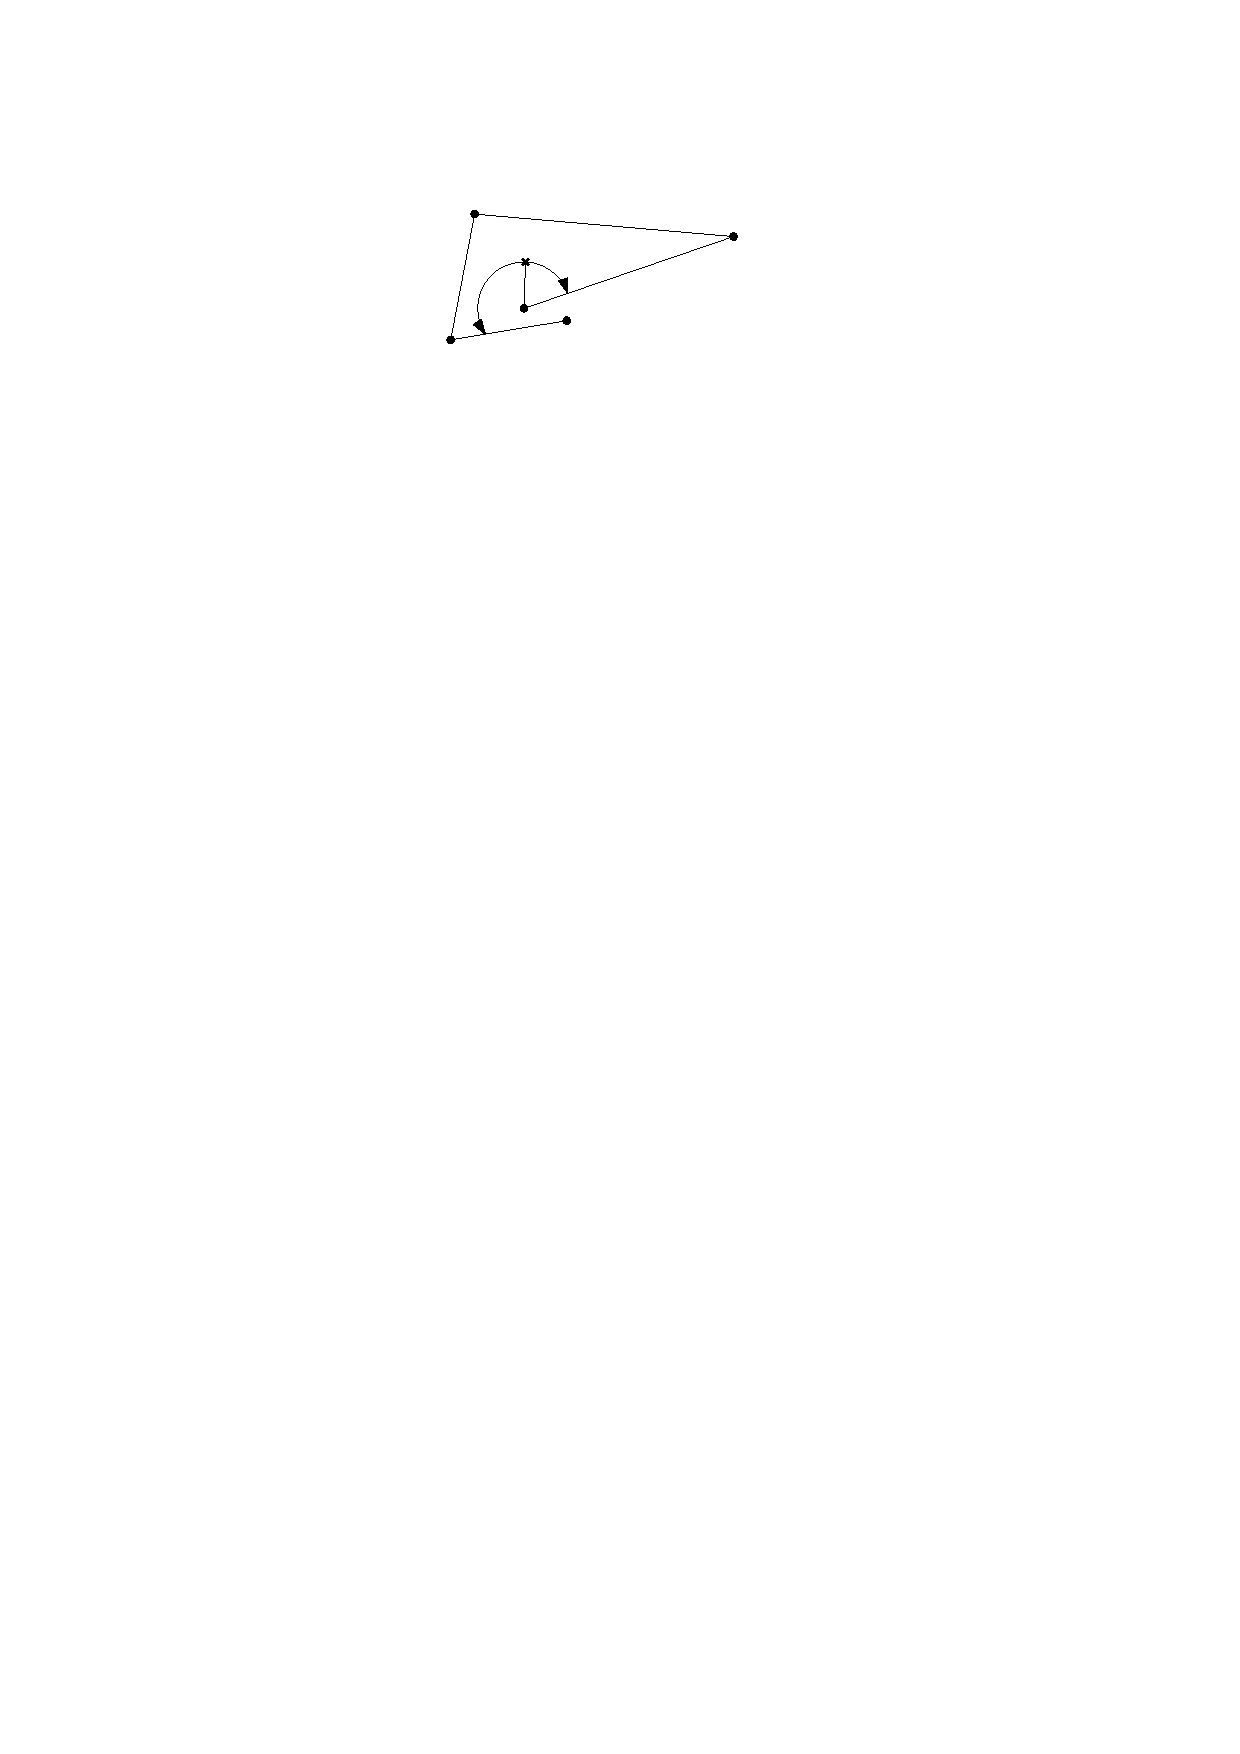
\includegraphics{graphics/freeJointPinnedJoint.pdf}
\end{center} 
\caption{The cross represents a free joint; the pinned joints are denoted as disks.  The range of motion shown by the arc describes the continous configuration space of the linkage.}
\end{figure} 

For illustrations in the remainder of this paper, free joints will be represented as crosses and pinned joints will be represented as disks.

\section{Polygonal Linkages}

\begin{figure}[h]
\begin{center}

\includegraphics[scale=1]{graphics/hingeOnThreeDistinctPolygons.pdf}
\end{center} 
\caption{(a) A polygonal linkage with a non-convex polygon and two hinge points corresponding to 
three polygons.  Note that hinge points correspond to two distinct polygons.(b) Illustrating that 
two hinge points can correspond to the same boundary point of a polygon.}
\label{fig:linkage-1}
\end{figure}
%describe how it is a generalization of Linkages.
A generalization of linkages are polygonal linkages where the edges of given lengths are replaced 
by rigid polygons.  Formally, a \textit{polygonal linkage} is an ordered pair $\left(\PP,\HH 
\right)$ where $\PP$ is a finite set of polygons and $\HH$ is a finite set of hinges; a 
\textit{hinge} $h\in \HH$ 
corresponds to two points on the boundary of two distinct polygons in $\PP$.  A \emph{realization} 
of a polygonal linkage is an interior-disjoint placement of 
congruent copies of the polygons in $\PP$ such that the points corresponding to each hinge are 
identified (Fig. \ref{fig:1}). 
A \textbf{realization with orientation} uses only translated or rotated copies of the polygons in $\PP$ (no reflections) and for each hinge, the cyclic order of incident polygons is given. 
The topology of a polygonal linkage can be represented by the \textbf{hinge graph}, a bipartite graph where the vertices correspond to polygons in $\PP$ and the hinges in $H$, and edges represent the polygon-hinge incidences.
This definition of realization rules well known geometric 
dissections (e.g. Fig. \ref{fig:polygonallinkage-4}).
%this is where the geometric dissection figure belongs
\begin{figure}[h]
\begin{center}
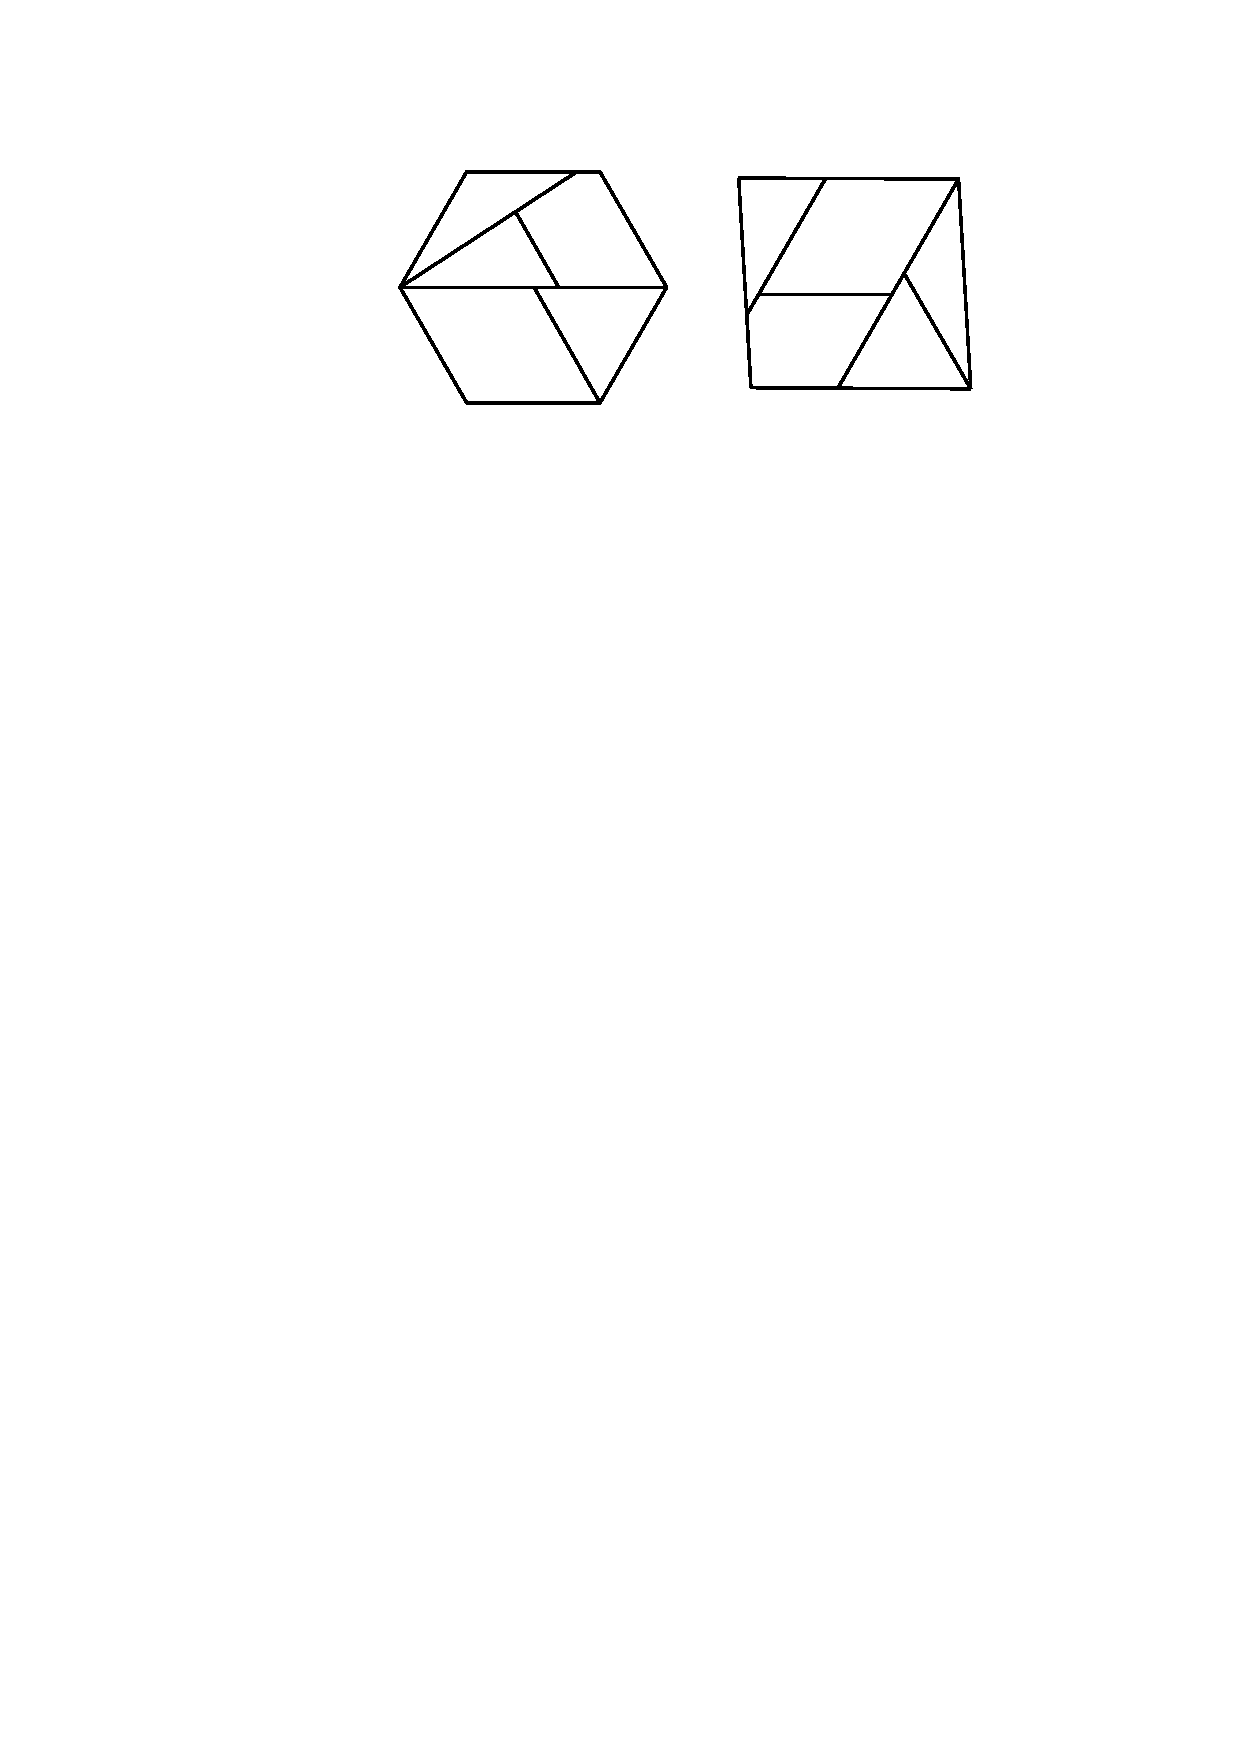
\includegraphics{graphics/GeometricDissectionBusschop.pdf}
\end{center}
\caption{Two configurations of polygonal linkage where the polygons touch on boundary segments 
instead of hinges.  These two realizations of the polygonal linkage are invalid to our definitions. 
 }
\label{fig:polygonallinkage-4}
\end{figure}

\begin{figure}[h]
\begin{center}
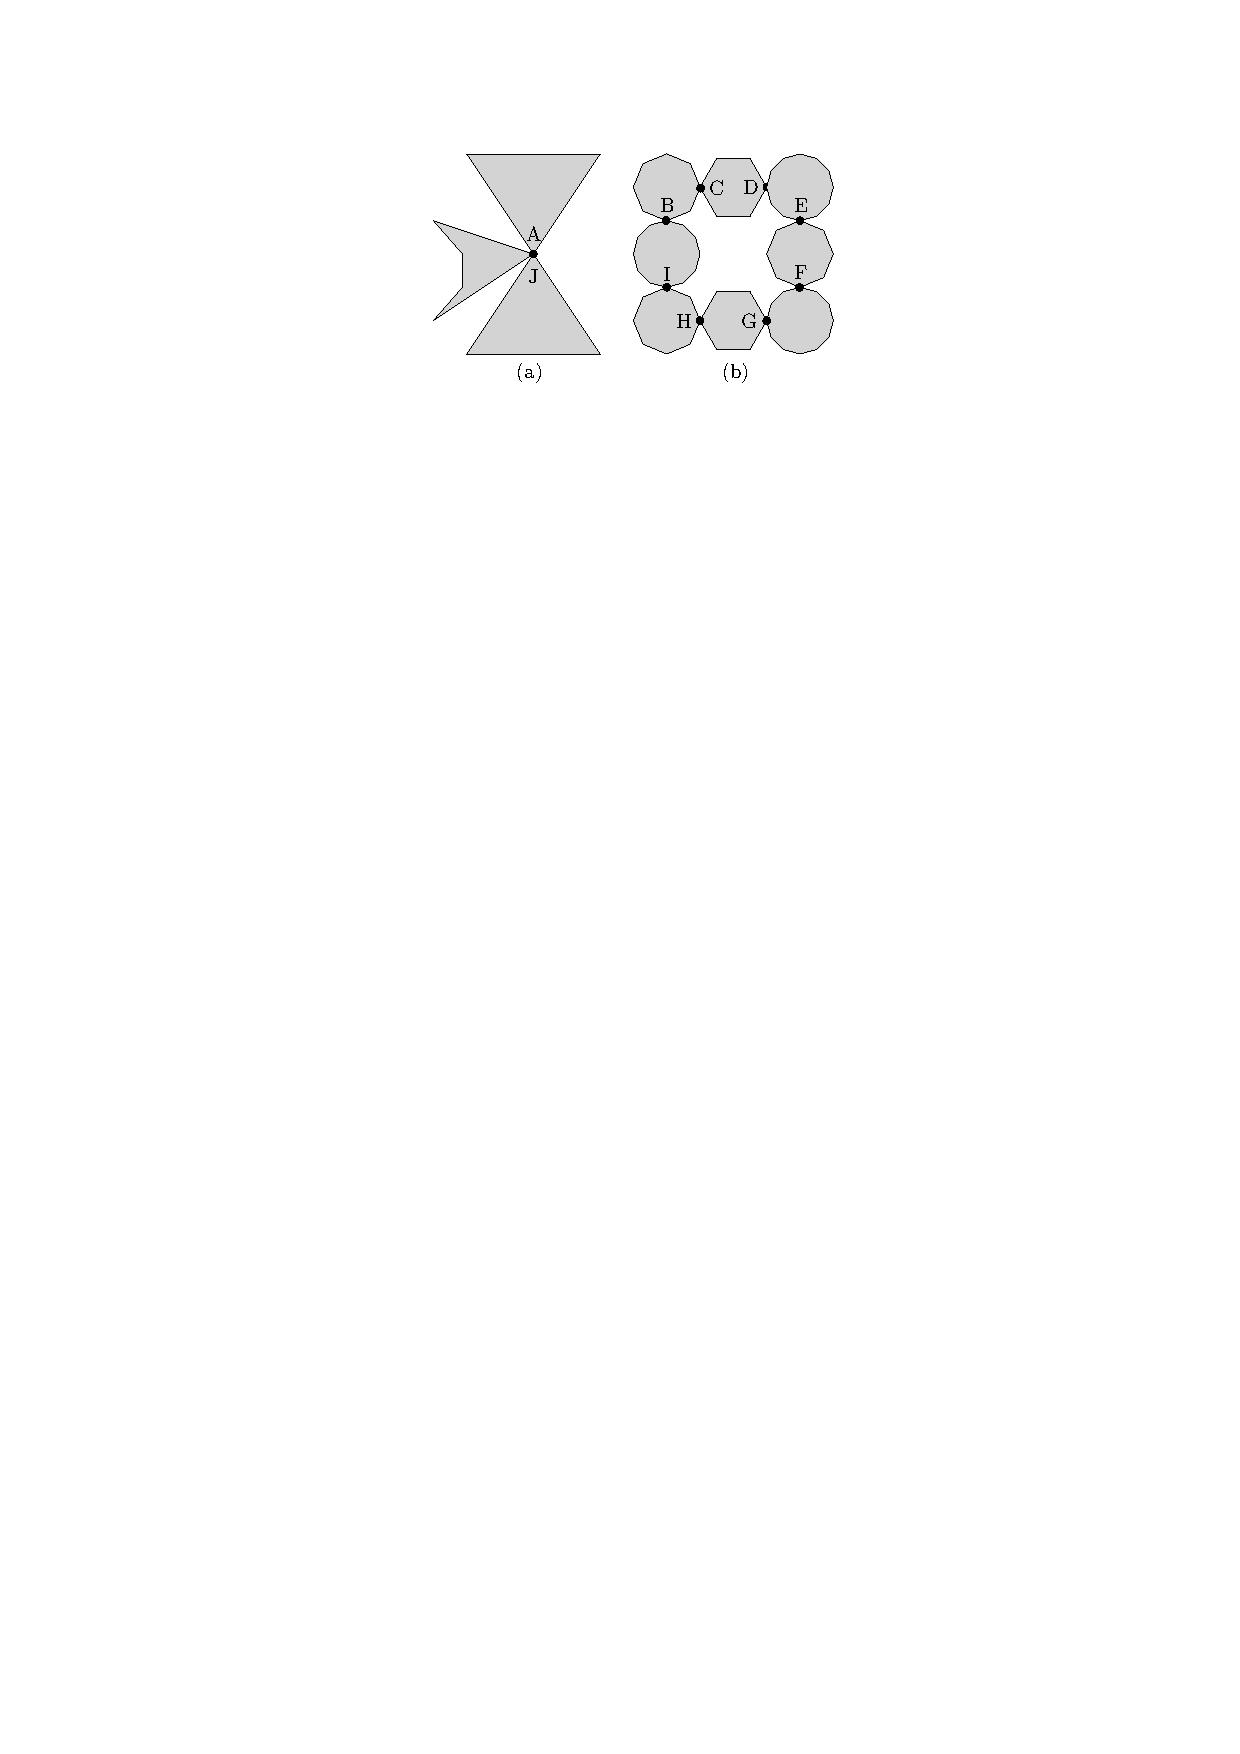
\includegraphics[scale=1]{graphics/linkageillustration.pdf}
\end{center} 
\caption{(a) A polygonal linkage with a non-convex polygon and a hinge point corresponding to three 
polygons.  (b) A polygonal linkage with 8 regular polygons.}
\label{fig:linkage-2}
\end{figure}


% For the remainder of this thesis, we'll focus on the polygonal linkages with the following 
% restrictions:
% \begin{enumerate}
% \item Embedded polygons must be convex, i.e. for any two embedded points $u,v \in P'$, the set:
% $$\left\lbrace u  \cdot t + (1-t) \cdot v : t \in [0,1] \right\rbrace \in P'$$
%  \item  Polygons can only intersect at hinge points.  No two polygons can intersect at 
% their boundary or interior with the exception of possible a hinge point.  
% \end{enumerate}
% 1.1.3. Disk graphs and problem definitions

% For the sake of simplicity, throughout this thesis we often refer to disks and their corre- sponding vertices synonymously. For example, we might simply say ’we create a disk D2 with radius r2 that touches disk D1’ instead of saying ’we create a vertex v2, a correspond- ing disk D2 with radius r2 and an edge between v2 and vertex v1 whose corresponding disk is D1’.
% Let G = (V, E) be a graph. We say that G has a realization as a disk intersection (touching) graph, if there exist a set of disks V and a bijection from V to V such that G = (G,V) is a disk intersection (touching) graph. In this case, we say G realizes G. Let Dv ∈ V be the disk of G corresponding to vertex v for any v ∈ V . A radius assignment for G is a function r : V → R+ that assigns a positive real number to each vertex of G. If the radius of disk Dv ∈ V is equal to r(v) for every v ∈ V , then G is said to respect r. A seed assignment for G is a function σ : V → R2 that assigns a point in the plane to each vertex ofG.Ifσ(v)∈Dv foreveryv∈V,thenGissaidtorespectσ.LetΓbeacombinatorial embedding for G. If G is a disk touching graph and if the cyclic order of disks touched by Dv corresponds to the cyclic order of edges incident to the vertex v for any v ∈ V , then G is said to respect Γ.
% We consider the following family of decision problems, in which the dots (...) are a place- holder for one, multiple or none of the enlisted variants.
% (Unit/ρ-bounded) Disk Intersection/Touching Graph Recognition (with ...): The problem instance is a graph G = (V, E) and the question is whether it is possible to realize G as a (unit/ρ-bounded) disk intersection/touching graph (which respects ...).
% • ... fixed Radii: ... a given radius assignment r for G.
% • ... fixed Embedding: ... a given combinatorial embedding Γ for G. • ... fixed Seeds: ... a given seed assignment σ for G.
% In particular, we consider the following problems:
% • Unit Disk Touching Graph Recognition (UDT)
% • Unit Disk Touching Graph Recognition with fixed Embedding (UDTE)
% • ρ-bounded Disk Touching Graph Recognition (ρ-BDT)
% • Disk Touching Graph Recognition with fixed Radii (DTR)
% • Disk Touching Graph Recognition with fixed Radii and Embedding (DTRE)
% • Disk Touching Graph Recognition with fixed Seeds (DTS)
% • Unit Disk Touching Graph Recognition with fixed Seeds (UDTS)
% • Unit Disk Touching Graph Recognition with fixed Seeds and Embedding (UDTSE)
% 1.2. Related work
% As mentioned in the beginning of this chapter, Koebe’s Theorem [Koe36] implies that the Disk Touching Graph Recognition problem can be solved in linear time. On the other hand, Hlinˇeny ́ and Kratochv ́ıl showed that the Disk Intersection Graph Recognition problem is NP-hard [HK01].
% A result by Breu and Kirkpatrick states that the Unit Disk Intersection/Touching Graph Recognition problems are NP-hard [BK98], implying that the Disk Intersection/Touching Graph Recognition with fixed Radii problems are also N P -hard. There exists some heuris- tics for generating disk touching graphs with fixed radii [Dor96, Ino11] for the application of cartogram generation.
% 6
% Breu and Kirkpatrick generalized their results by showing that the ρ-bounded Disk Inter- section/Touching Graph Recognition problems are NP-hard for any fixed ρ ≥ 1 [BK96]. Alam et al. [AEG+14] argue that for any tree, for any cactus (which is a connected graph in which each edge is contained in at most one cycle), for any k-outerplanar graph with bounded maximum degree and k ∈ O(log n) and for any planar graph with bounded tree- depth there exists a realizing ρ-bounded disk touching graph where ρ is a polynomial in the number of vertices.
% Atienza et al. show that the Disk Touching Graph Recognition with fixed Seeds problem is NP-hard [AdCC+12].








\section{Disk Arrangements}
%Circle packing theorem: For every connected simple planar graph G there is a circle packing in the plane whose intersection graph is (isomorphic to) G.
% A disk D is a region in the plane bounded by a circle. A disk can be uniquely described by its bounding circle’s radius r ∈ R+ and center c ∈ R2. A disk is called closed if it contains the points of its bounding circle and open otherwise. A disk intersection graph G = (G, V) consists of a graph G = (V,E), a set of closed disks V and a bijection from the set of vertices V to V such that two vertices of V are adjacent in G if and only if their corresponding disks in V intersect. A disk touching graph G = (G, V) is a disk intersection graph such that the interiors of the disks in V are pairwise disjoint. The centers of the disks in V together with straight-line segments that connect the centers of all pairs of touching disks induce a planar drawing of G. In a unit disk intersection (touching) graph all disks share one uniform radius. In a ρ-bounded disk intersection (touching) graph the radius of all disks is taken from the interval [1, ρ] for a value ρ ≥ 1. Note, that a 1-bounded disk intersection (touching) graph is a unit disk intersection (touching) graph.





 A \textit{disk arrangement} is a set of interior disjoint disks, $D$.  
 If for any pair of disks in $D$ intersect at a boundary point, they are said to be in contact (kissing).
\begin{figure}[!hbtp]
\begin{center}
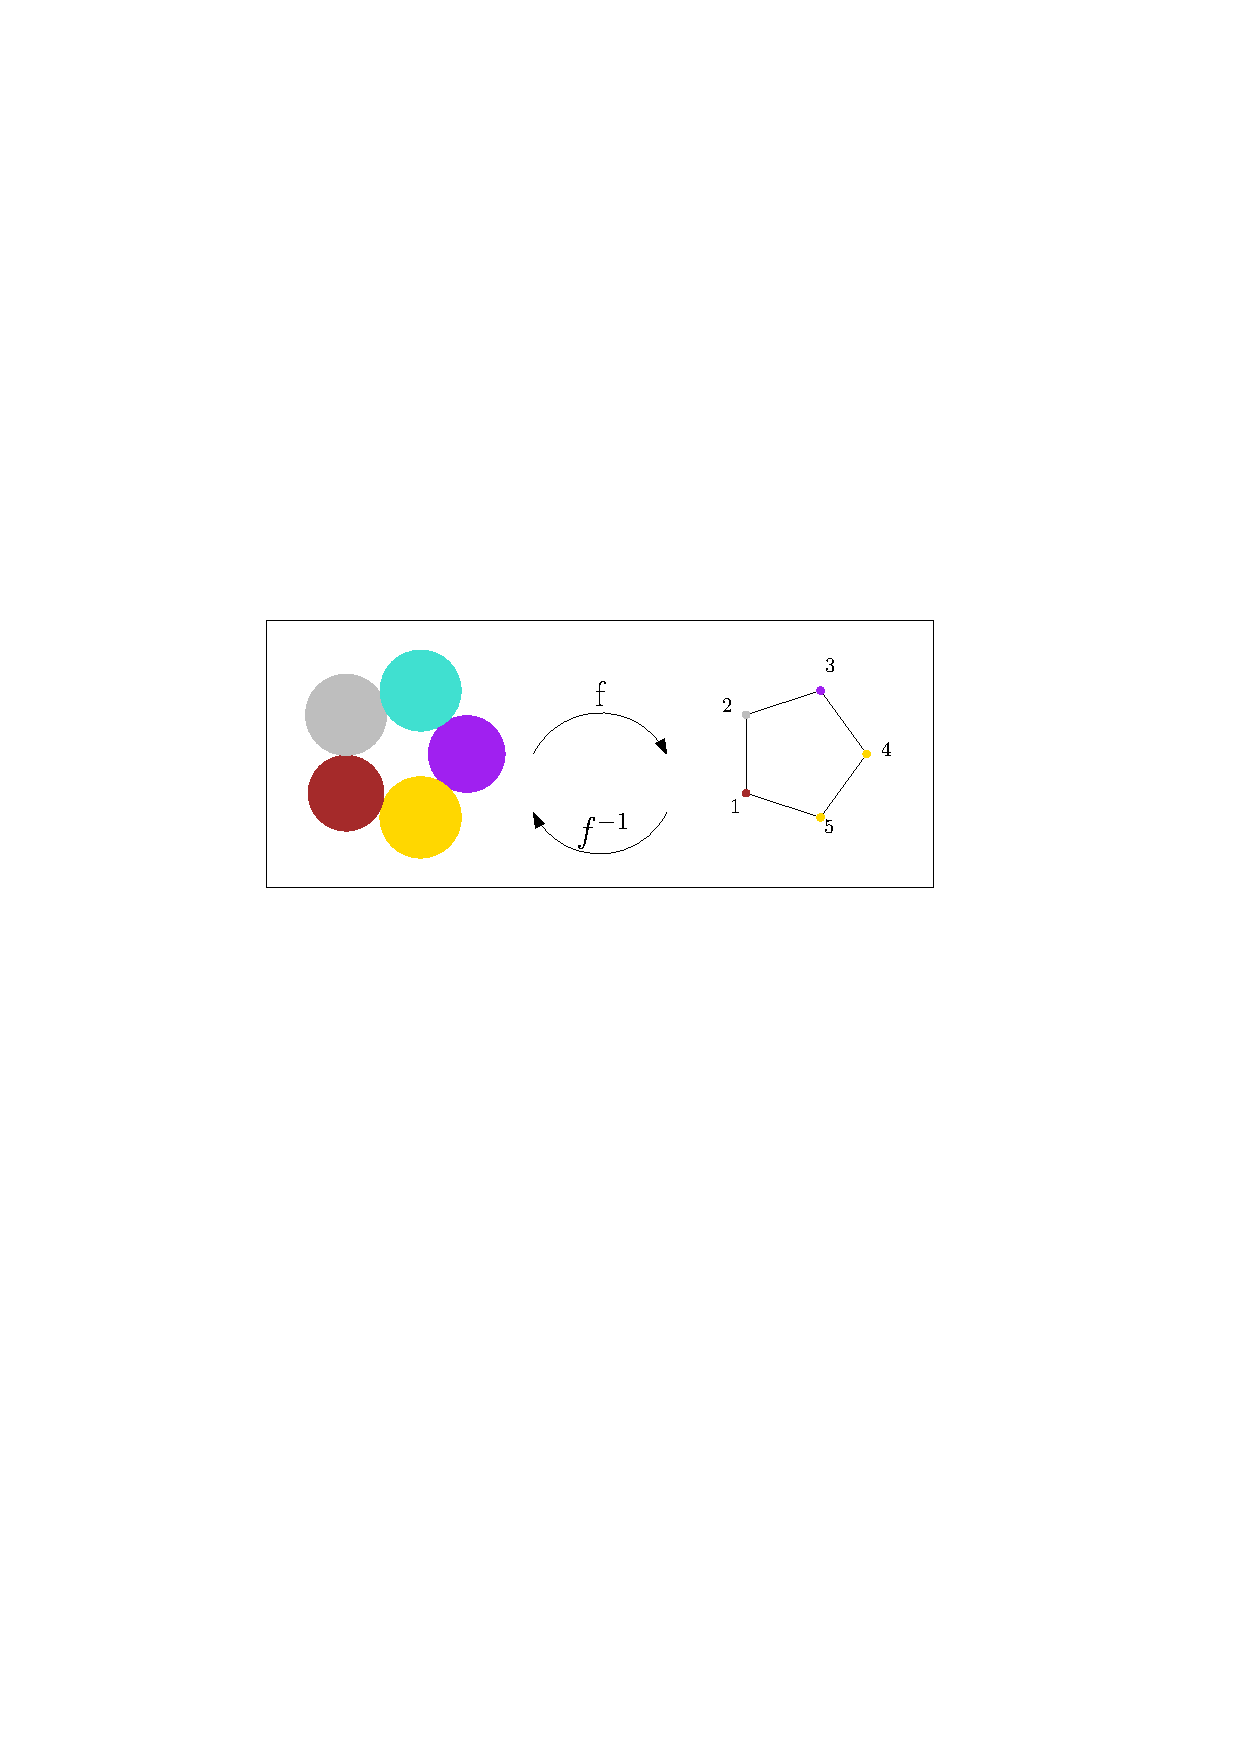
\includegraphics[scale=1]{graphics/diskPackingTheoremExample.pdf}
\end{center} 
\caption{This example represents a disk arrangement and its contact graph.}
%Figure shows a 5-cycle with a unique realization of a disk arrangement.
\label{fig:DiskArrangement-1}
\end{figure}
A \textit{contact graph} $G=(V,E)$ corresponding to a given disk arrangement where there is a bijection $b_V: V \mapsto D$ and a bijection that maps an edge $e_{i,j} \in E$ to an interior disjoint pair of disks $d_i$, $d_j \in D$ (see Figure \ref{fig:DiskArrangement-1}).
Given a disk arrangement, the contact graph can be thought of as a linkage because the distance between two kissing disk equal the sum of radii.  
However if the two disks don't kiss, the distance between their centers is strictly greater than the sum of their radii.
Given a disk arrangement, the contact graph can be thought of as a linkage because the distance between two kissing disk equal the sum of radii.  
However if the two disks don't kiss, the distance between their centers is strictly greater than the sum of their radii.

Koebe's theorem states that for every planar graph $G$, there exists a planar disk arrangement whose contact graph is $G$ \cite{koebe1936kontaktprobleme}.
This motivates the question of whether a planar graph $G$ is a contact graph of a disk arrangement with given radii.
The radii can be given by a weight function.
Let $\omega: V \mapsto \bbR^+$ be the \textit{weight function}.  
$\omega$ assigns a weight to each vertex in $V$.  
Let $\Pi:V \mapsto \bbr^2$ be that planar mapping of vertices.
%$D$ \textit{respects radii assignments} if for every $v \in V$ such that $b_V(v) = D_v$, $\omega(v)$ is the radius of $D_v$.    
%$D$ \textit{respects center assignments} if for every $v \in V$, $\Pi(v)$ is the center of $D_v$.  
%Note that if $\omega$ respects radii assignments, then it can be equivelently said that the linkage $(G,\ell)$ with length assignment $\ell$ also respects radii assignments.  
%In this thesis, unless otherwise stated we assume that the contact graph associates to an $\omega$ and $\Pi$ mapping that respect radii and center assignments.
%we may also interchange contact graph with linkage.



% For the sake of simplicity, throughout this thesis we often refer to disks and their corre- sponding vertices synonymously. For example, we might simply say ’we create a disk D2 with radius r2 that touches disk D1’ instead of saying ’we create a vertex v2, a correspond- ing disk D2 with radius r2 and an edge between v2 and vertex v1 whose corresponding disk is D1’.
% Let G = (V, E) be a graph. We say that G has a realization as a disk intersection (touching) graph, if there exist a set of disks V and a bijection from V to V such that G = (G,V) is a disk intersection (touching) graph. In this case, we say G realizes G. Let Dv ∈ V be the disk of G corresponding to vertex v for any v ∈ V . A radius assignment for G is a function r : V → R+ that assigns a positive real number to each vertex of G. If the radius of disk Dv ∈ V is equal to r(v) for every v ∈ V , then G is said to respect r. A seed assignment for G is a function σ : V → R2 that assigns a point in the plane to each vertex ofG.Ifσ(v)∈Dv foreveryv∈V,thenGissaidtorespectσ.LetΓbeacombinatorial embedding for G. If G is a disk touching graph and if the cyclic order of disks touched by Dv corresponds to the cyclic order of edges incident to the vertex v for any v ∈ V , then G is said to respect Γ.
% %By Koebe's Theorem, every disk arrangement embedded in the plane has a contact graph.
% A \textit{contact graph} represents vertices as interior disjoint disks and by representing edges as as points of intersections (contact), \textit{kissing points} between two disks.  
% The graph corresponding to a given disk arrangement, $\DD$, is said to be the \textit{contact graph}. 
% An ordered disk arrangement preseves the  cyclic order of neighborings disks. 
% %A \it{disk arrangement} is a set, $\DD$, of pairwise interior-disjoint disks in the plane, 
% %$\DD=\left\lbrace C_i \right\rbrace_{i = 1}^n $.


%What is not obvious is when given a graph with positive weights, does there exist a planar drawing?
%Some variants of these problems were known to be NP-Hard.
For planar graphs with positive weighted vertices, we pose two realizability problems:
\begin{prob}[Unordered Realizibility Problem for a Contact Graph]\label{problem:UnorderedContactGraph}
Given a planar graph with positive weighted vertices, is it a contact graph of some disk arrangement where the radii equal the vertex weights?
\end{prob}
\begin{prob}[Ordered Realizibility Problem for a Contact Graph]\label{problem:OrderedContactGraph}
Given a planar graph with positive weighted vertices and a combinatorial embedding, is it a contact graph of some disk arrangement where the radii equal the vertex weights and the counter-clockwise order of neighbors of each disk is specified by the combinatorial embedding?
\end{prob}

An instance of Problem \ref{problem:UnorderedContactGraph} is shown in Figure \ref{fig:DiskArrangement-1} where the cycle graph $C_5$ is the contact graph of unit disks.
It is not difficult to see that there exists a planar graph with positive weights with no realizable disk arrangement.
Consider the a star graph with 6 leafs, each vertex with unit weight.
In any realization, the angle between two consecutive edges must be greater than $\frac{\pi}{3}$. 
The sum of 6 angles is $2 \pi$ however, the sum of 6 consecutive angles is greater than $2\pi$.
The contradiction shows that no realization is possible (refer to Figure \ref{figure:starweel}).
Note that with the wheel graph $W_7$ is realizable as a contact graph of unit disks.

Every path with arbitrary positive radii is realizable as a contact graph, place the vertices on a line.
We show that not all binary trees are realizable, even with unit disks.% of unit radii.
Consider the balanced binary trees of depth $i$ $\left\lbrace T_i \right\rbrace_{i=1}^\infty$ with unit weights on the vertices (see Figure \ref{fig:circlePacking-1}).
These trees are not realizable for sufficiently large $i$.
\begin{figure}[!htbp]\label{fig:circlePacking-1}
\begin{center}
    %add desired spacing between images, e. g. ~, \quad, \qquad etc.
    %(or a blank line to force the subfigure onto a new line)
  \begin{subfigure}[b]{0.21\textwidth}
	  \includegraphics[width=\textwidth]{graphics/BinaryTree1.pdf}
	  \caption{Binary tree $T_2$.}
	  \label{fig:circlePacking1-1}
  \end{subfigure}
  \begin{subfigure}[b]{0.21\textwidth}
	  \includegraphics[width=\textwidth]{graphics/BinaryTree2.pdf}
	  \caption{Binary tree $T_3$.}
	  \label{fig:circlePacking1-2}
  \end{subfigure}
  \begin{subfigure}[b]{0.21\textwidth}
	  \includegraphics[width=\textwidth]{graphics/BinaryTree3.pdf}
	  \caption{Binary tree $T_4$.}
	  \label{fig:circlePacking1-3}
  \end{subfigure}
  \begin{subfigure}[b]{0.21\textwidth}
	  \includegraphics[width=\textwidth]{graphics/BinaryTree4.pdf}
	  \caption{Binary tree $T_5$.}
	  \label{fig:circlePacking1-4}
  \end{subfigure}
  \caption{ We show the linkages $T_2$ through $T_5$ with distance 2 between adjacent vertices.  }
\end{center} 
\end{figure}
%To show that as $i \rightarrow \infty$, the corresponding disk arrangement will not have a drawing.  
%We construct the disk arrangement as follows: (1) place a disk of unit radius centered at origin; (2) for each disk continue to add two non-intersecting kissing disks of unit radius to it.  
%To illustrate, see Figure \ref{fig:circlePacking-1}:
Let $i$ be a positive integer and suppose that $T_i$ is a contact graph of unit disks.
The balanced binary tree $T_i$ has $2^i -1$ vertices.
The total area of the disks is $\left( 2^i -1 \right)^2 \cdot \pi$.
We now derive an upper bound for this area.
%Suppose the root of the disk arrangement is centered at origin.
Suppose the disk corresponding to the root of the tree is centered at the origin.
The centers of the disks at level $j$ are at a distance at most $2\cdot (j-1)$ away from the origin.
The centers of all disks are at distance at most $2 \cdot (i -1)$ away from the origin.
All unit disks are contained in a disk of radius $2i-1$ centered at the origin.
The total area of the disks is at most $(2i-1)^2$.
%Let the total area of the disks arrangement be the sum of the areas of the disks. 
A upper bound of the total area of the disk arrangement is the area of the bounding box of the disks.
The upper bound of the 


\begin{figure}[!htpb]\label{fig:circlePacking-2}
\begin{center}
    %add desired spacing between images, e. g. ~, \quad, \qquad etc.
    %(or a blank line to force the subfigure onto a new line)
  \begin{subfigure}[b]{0.24\textwidth}
	  
\includegraphics[width=\textwidth]{graphics/degree2arrangement.pdf}
	  \caption{A disk arrangement with two layers of disks}
	  \label{fig:circlePacking2-1}
  \end{subfigure}
  \begin{subfigure}[b]{0.24\textwidth}
	  
\includegraphics[width=\textwidth]{graphics/degree3arrangement.pdf}
	  \caption{A disk arrangement with three layers of disks}
	  \label{fig:circlePacking2-2}
  \end{subfigure}
  \begin{subfigure}[b]{0.24\textwidth}
	  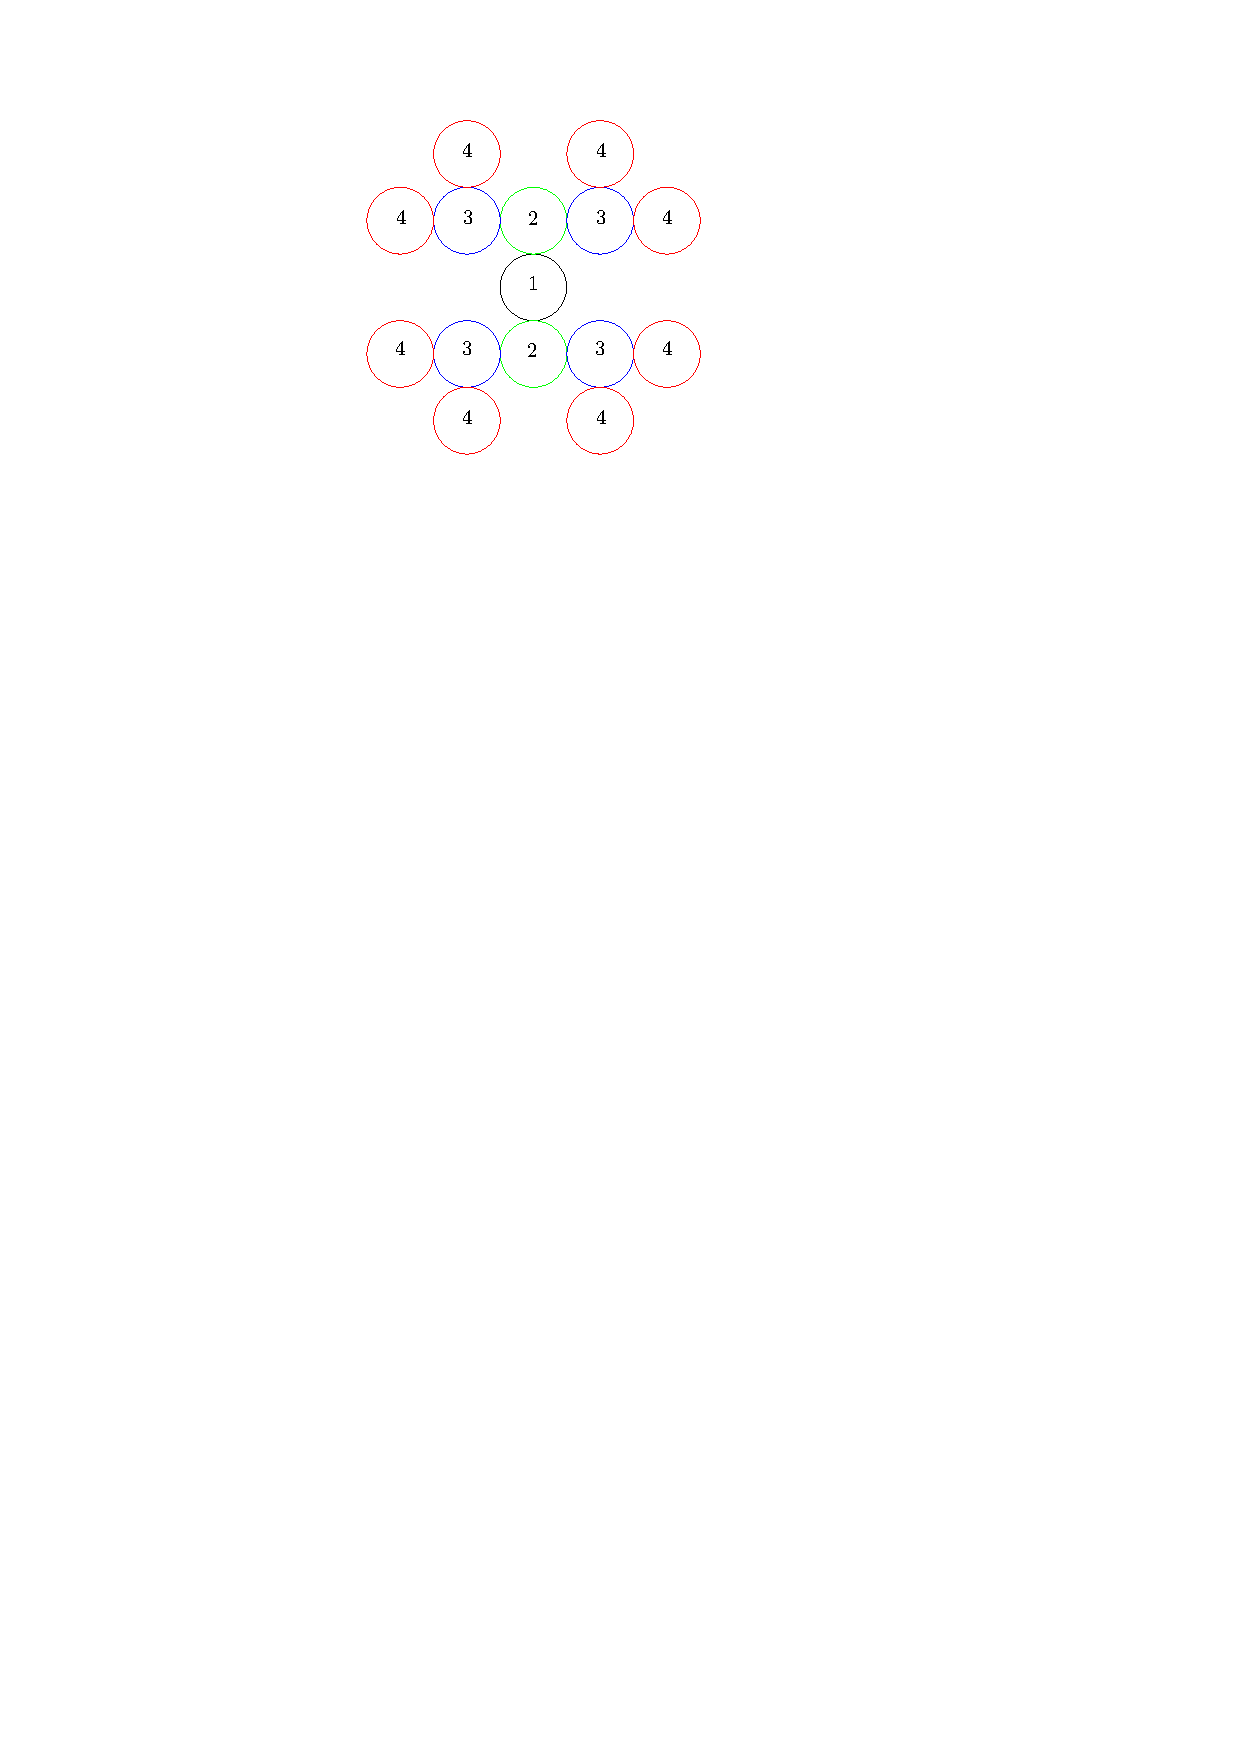
\includegraphics[width=\textwidth]{graphics/degree4arrangement.pdf}
	  \caption{A disk arrangement with four layers of disks}
	  \label{fig:circlePacking2-3}
  \end{subfigure}
  \begin{subfigure}[b]{0.24\textwidth}
	  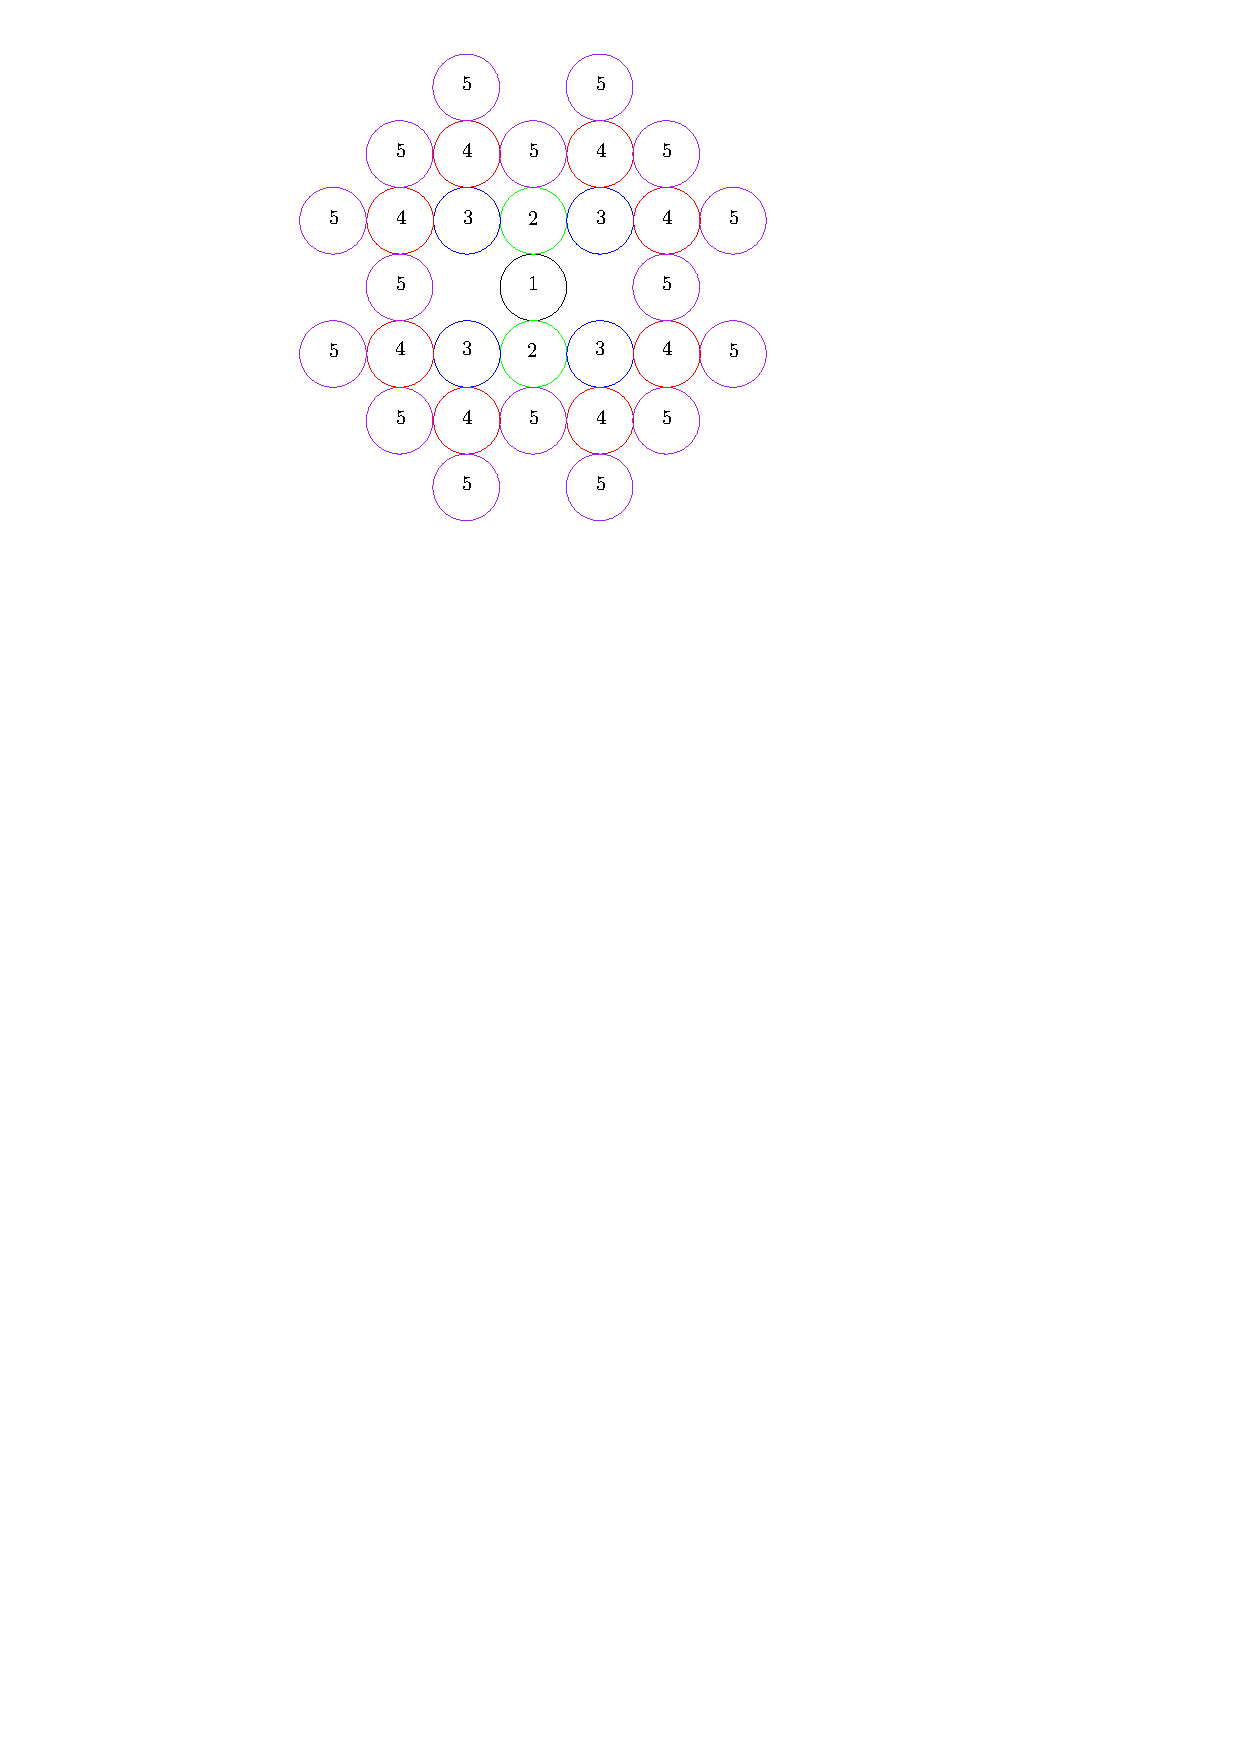
\includegraphics[width=\textwidth]{graphics/degree5arrangement.pdf}
	  \caption{A disk arrangement with five layers of disks}
	  \label{fig:circlePacking2-4}
  \end{subfigure}
\end{center} 
\caption{For $i=2,3,4,5$ the tree $T_i$ is a contact graph of unit disks.}\label{fig:circlePacking-1}
\end{figure}
% The first round has one unit disk.  
% The next round, two unit radii disk are in contact with the first, i.e. Figure \ref{fig:circlePacking1-1}.
% The subsequent rounds are shown in Figures \ref{fig:circlePacking1-2}, \ref{fig:circlePacking1-3}, and \ref{fig:circlePacking1-4}.  
% For each round $i$ we are adding $2^{(i-1)}$ disks, each with an area of $\pi$.  
% The area that the disk arrangement is bounded at round $i$ is a box of length $2\cdot (2\cdot (i-1)+1)$ totalling to an area of $(4\cdot i^2 - 4\cdot i + 1)$.  
% Meanwhile the total area of the disk arrangement at $i$ is $\pi \cdot (2^i - 1)$.  The exponential growth rate of the disk packing will exceed its bounded area for sufficiently large $i$, i.e. pick $i \geq 6$.
Figure \ref{fig:circlePacking-2} shows the first four non-trivial trees as a contact graph of unit disks.
Every disk at level up to $i$ is contained in a disk of radius $2\cdot i - 1$ centered at the origin.
The total area of the disk arrangement is $(2\cdot i -1)^2 \cdot \pi$. 
When $i\geq 8$ we have a contradiciton.%the total area of the disk arrangement exceeds the total bounded area and thus we have a contradiction.

\begin{figure}[!htbp]\label{fig:circlePacking-3}
\begin{center}
    %add desired spacing between images, e. g. ~, \quad, \qquad etc.
    %(or a blank line to force the subfigure onto a new line)
  \begin{subfigure}[b]{.48\textwidth}
  \begin{center}
	  \includegraphics[scale=.9]{graphics/OrderedDiskArrangementExample1.pdf}
	  \label{fig:circlePacking3-1}
	  \end{center}
  \end{subfigure}
  \begin{subfigure}[b]{0.48\textwidth}
  \begin{center}
	  \includegraphics[scale=.9]{graphics/OrderedDiskArrangementExample2.pdf}	  
	  \label{fig:circlePacking3-2}
	  \end{center}
  \end{subfigure}
  \caption{Consider these two ordered disk arrangements where A and B are in the concentric rings of disks.  The large disks are in contact to A and B respectively.  
  If A and B are adjacent, then there is a restriction of how large the size of the disks can be that are attached to them as seen in on the left.  
  Whereas if A and B are not adjacent in this disk arrangment as shown on the right, the size of the kissings disks could be arbitrarily large.}
\end{center} 
\end{figure}

There are instances where a planar graph with weights admits a realization but the cyclic order of neighbors may not be the same as the combinatorial embedding.
Define $G$ as follows: start with a star centered at $C$ and with 6 leafs, $A_1$ through $A_6$; attach two leafs, $B_1$ and $B_2$, to $A_1$ and  $A_2$ respectively (see  Figure \ref{fig:circlePacking-3}).
Let the weight of $C$ be $1+\epsilon$ for sufficiently small $\epsilon > 0$.
The neighbors of $C$ have unit weight.
The weights of the two leaves have weight $\frac{1}{\epsilon}$/
The right of Figure \ref{fig:circlePacking-3}) shows a realization where $A_1$ and $A_2$ are in opposite position of the counter-clockwise order around $C$.
If $A_1$ and $A_2$ are required to be consecutive in the counter-clockwise order around $C$, there is no realization.
%as epsilon goes to 0 the half planes approximates the disks and so the disks will intersect as well.  label everything, draw halff planes, epsilon and delta, 1/epsilon.

Suppose there is a realization where $A_1, \ldots, A_6$ are in the counter-clockwise order around $C$ (see Figure \ref{{fig:DiskArrangement-4}}).
If $\epsilon>0$ is sufficiently small, then the centers of of $A_1, \ldots, A_6$ are arbitrarily close to the vertices of a regular hexagon.
Consider the common tangent lines between $A_1$ and $B_1$ and $A_2$ and $B_2$.
The possible position of tangent line between $A_1$ and $B_1$ ranges from the common tangent line of $A_1$ and $A_6$ to the common tangent line of $A_1$ and $A_2$.
Similarly, The possible position of tangent line between $A_2$ and $B_2$ ranges from the common tangent line of $A_2$ and $A_3$ to the common tangent line of $A_1$ and $A_2$.
In any position, the common tangent lines between $A_1$ and $B_1$ and $A_2$ and $B_2$ intersect.
If $\frac{1}{\epsilon}$ is sufficiently large, then the disks $D_1$ and $D_2$ also intersect.
This contradicts that there is a realization.
\begin{figure}[!hbtp]
\begin{center}
\includegraphics[scale=1]{graphics/orderedPlaneIntersection.pdf}
\end{center} 
\caption{This example represents a disk arrangement and its contact graph.}
%Figure shows a 5-cycle with a unique realization of a disk arrangement.
\label{fig:DiskArrangement-4}
\end{figure}
Figure \ref{fig:circlePacking-3} shows how an ordered contact graph may not be realizable.  
On the left, it shows a limitation on the weights of the disks that are in contact with disks A and B. 
On the right, the figure shows the order where A and B are on opposing ends of the ring of disks and can allow of arbitrary size of wieghted disks in contact with A and B.
% Figure \ref{fig:orderedFaces.pdf} shows three polygons with a common hinge.
% In the counter-clockwise order $(A,B,C)$, the polygonal linkage admits a realization whereas in the counter-clockwise order $(A,C,B)$, it does not admit a realization.
% \subsection{Disk Packing Confinement Problem}

% Given inputs of radii 
% By adding constraints to the embeddings of disk arrangements, we can devise realizability problem 
% by a volume argument.
% \begin{enumerate}%1,2,3,4....
% \item Round 1: Start with a disk of unit radius.
% \item Round 2: Add two kissing disks, each of diameter 2, that do not intersect with any other 
% disk (they 
% may kiss other
% disk).
% \item Round 3 and Higher: For each new kissing disk added, add two more non-intersecting kissing 
% disks of diameter 2 to it.
% \end{enumerate} 


% Figure (\ref{fig:circlePacking-1}) illustrates the iterative problem.  The problem with this is that 
% the area in
% which is necessary to contain this disk growing disk arrangement will exceed the area needed to 
% contain it.





%The corresponding intersection graph of a disk packing is a graph whose vertices are the disks and edges correspond to two disks that contact each other.
% \section{Disk Arrangements}
% It turns out the disk arrangements are an equivalent way to to represent plane graphs.  By 
% representing vertices as interioir disjoint disks and by representing edges as as points of 
% intersections (contact), \textit{kissing 
% points} between two disks.  The graph corresponding to a given disk arrangement, $\DD$, is said to 
% be the \textit{contact graph}. A \it{disk arrangement} is a set, $\DD$, of pairwise 
% interior-disjoint disks in the plane, 
% $\DD=\left\lbrace C_i \right\rbrace_{i = 1}^n $.
% $\left\lbrace C_i \right\rbrace_{i = 1}^n $ such that for any circle $C \in \left\lbrace C_i 
% \right\rbrace_{i = 1}^n$, $C$


% %(fig 1) a disk arrangement
% %(fig 2) an equivalent contact graph to (fig 1)
% A classical result by Thurston and Koebe is that every disk arrangement embedded into the plane had 
% a corresponding plane graph.
% \begin{thm}[\ref{stephenson2005introduction}Disk Packing Theorem]\label{thm2-1}
% For every graph $G$, there is a disk arrangement in the
% plane whose contact graph is isomorphic to $G$.
% \end{thm}

% %add a paragraph with atoms of molecules are modeled with disks and balls of fixed radii. The 
% %if two disks are in contact, then the  distance between their centers  = the sum of the radii
% %conclude: disk arrangements are better models for representing atoms and molecules fixed distance 
% % betweeen atoms
% \begin{prop}
%  For every linkage $L$, there is a disk arrangement in the
% plane whose contact graph is isomorphic to $L$.
% \end{prop}



% \begin{enumerate}%1,2,3,4....
% %\item Introduce the circle packing theorem.
% \item Show the relation between polygonal linkages and disk arrangengements.
% \end{enumerate} 
% % \subsubsection{Ordered Disk Arrangement}
% Suppose we're given a tree. By the disk packing theorem we can ascertain a sense of order for the 
% isomorphic disk packing.  An \textit{ordered disk arrangement} is a rooted tree in which the 
% counter-clockwise ordering of adjacent vertices.
% % 


% The embedding problems for trees and corresponding disk arrangements are as follows:
% \begin{prob}[Unordered Realizibility Problem for the Tree]\label{problem:UnorderedContactGraph}
% For a tree with positive weights for the verticies, it asks whether it is a contact graph of some 
% disk arrangement where the radii are equal to the vertex weights.
% \end{prob}

% \begin{prob}[Ordered Realizibility Problem for the Tree]\label{problem:OrderedContactGraph}
% For a tree with positive weights for the vertices, it asks whether its corresponding graph is the 
% ordered contact graph of some disk arrangement where the radii equal the vertex weights.
% \end{prob}

\section{Configuration Spaces}
\begin{quote}
Just as one can compose colors or forms, so one can compose motions.
\end{quote}
{\raggedright{}Alexander Calder, 1933}

Recall Figure \ref{fig:HingedHaberdasher} illustrating the hinged dissection that formed a square and triangle and several drawings of the hinged dissections that simulate the motion of moving the polygons around the hinge points to form each shape.  The set of all drawings in that motion represents the \textit{configuration space} for that polygonal linkage.  In this section we will formally describe the configuration space for each object we've drawn thus far.


% We'd like to describe motions and range of motions of embedded graphs, linkages, polygonal 
% linkages, and disk arrangements.  Table \ref{table:configurationSpace-1} provides the definition of 
% \textit{reconfiguration} for each type of object covered so far:
% \begin{center}
% \begin{table}[htbp!]
% \begin{tabular}{|p{.2\textwidth}|p{.79\textwidth}|}
% \hline
% Object Type&Definition of Reconfiguration\\\hline
% Graph Embeddings&a continuous motion of the vertices that never causes the edges to 
% intersect.\\\hline
% Linkage&a continuous motion of the vertices that preserves the lengths of the edges and never 
% causes 
% the edges to intersect.\\\hline
% Polygonal Linkage&a continuous motion of polygons that preserves shapes of polygons, hinge point 
% pairings, and never causes the polygonal sides to intersect.\\\hline
% Disk Arrangement&a continuous motion of disks that preserves disk radii, pairs of contact points, 
% and never causes disks to intersect.\\\hline
% \end{tabular}\label{table:configurationSpace-1}
% \end{table}
% \end{center}




% For graphs, a \textit{reconfiguration} is a continuous motion of 
% the vertices that preserve the length edges and never cause edges to collide \cite{AKR+04}.  For 
% polygonal linkages, a reconfiguration is 

\subsection{Configuration Spaces of Graph Drawings}
Recall that for a graph drawing we have an injective mapping $\Pi : V \mapsto \bbR^{2}$ which maps vertices to distinct points in the plane.  %and for each edge $\curlybraces{u,v} \in E$, a straight line segment, $c_{u,v}:[0,1]\mapsto \bbR^2$ such that $c_{u,v}(0) = \Pi(u)$ and $c_{u,v}(1) = \Pi(v)$, and does not pass through other vertices.
The mapping $\Pi$ uniquely determines each edge.
An edge $\curlybraces{u,v} \in E$, is mapped to a straight line segment, $c_{u,v}:[0,1]\mapsto \bbR^2$ such that $c_{u,v}(0) = \Pi(u)$ and $c_{u,v}(1) = \Pi(v)$, and does not pass through other vertices.
%For each vertex of $G$, the embedding of the vertex lies in the plane, i.e. $\Pi(v) \in \bbR^2$.  
Let $\DD_G$ be the set of all drawings of the graph $G$.  
By labelling the vertices of $G$, e.g. $v_1, v_2, \dots, v_k, \dots, v_{n}$, we can create a mapping from $\mu: \DD_G \mapsto \bbR^{2\vert V \vert}$ where the coordinates of $\Pi(v_k)$ are the $(2k)^\text{th}$ and $(2k+1)^\text{st}$ coordinates in $\bbR^{2\vert V \vert}$.  
$\mu(\Pi)$ is a configuration.
The configuration space is the set of $\mu(\Pi)$ for all drawings $\Pi$.  

\subsection{Configuration Spaces of Linkages}

Consider drawings of a graph that respects the length assignment.  
A \textit{realization} of a linkage, $(G,\ell)$, is a drawing of a graph, $\Pi$, such that for every edge $\{u,v\} \in E$, $\ell\left( \{u,v\} \right) = \left\vert \Pi(u) - \Pi(v) \right\vert = \left\vert \Pi(v) - \Pi(u) \right\vert$. 
A \textit{plane realization} is a plane drawing with the property, $\ell\left( \{u,v\} \right) = \left\vert \Pi(u) - \Pi(v) \right\vert$.
First let's define the space of realizations for a corresponding linkage, i.e.:
$$P_{(G,\ell)} = \set{\Pi\in \DD_G }{\forall \{u,v\} \in E\text{, }\ell\left( \{u,v\} \right) = \left\vert \Pi(u) - \Pi(v) \right\vert}$$
With respect to $P_{(G,\ell)}$, we can establish a configuration space that allows one to study problems of motion.  
For each vertex of $G$, the drawing of the vertex lies in the plane, i.e. $\Pi(v) \in \bbR^2$.  
By enumerating each vertex of $G$, e.g. $v_1, v_2, \dots, v_k, \dots, v_{n}$, we can create a mapping from $\mu: P_{(G,\ell)} \mapsto \bbR^{2\vert V \vert}$ where the corresponding coordinates of $\Pi(v_k)$ are in the $(2k)^\text{th}$ and $(2k+1)^{st}$ coordinates in $\bbR^{2\vert V \vert}$.  
The configuration space is $\mu\lr{P_{(G,\ell)}}$.  

Using standard definitions from real analysis, we can begin to pose problems about linkages with respect to a corresponding configuration space.  
A continuous function $\gamma: [0,1]\mapsto \mu\lr{P_{(G,\ell)}}$ is a path from a realization $\gamma(0)$ to another realization $\gamma(1)$.
$\gamma$ can be thought of as an animation of drawings that starts at $\gamma(0)$ and ends at $\gamma(1)$.
%corresponds to the mapping of a realization of a linkage $\Pi_0$ and $\gamma(1)$ corresponds to another realization of a linkage $\Pi_1$.  
%If for any two elements $a,b \in \mu(P)$ that there exists a continuous path $\gamma$ such that $\gamma(0)=a$ and $\gamma(1)=b$, $\mu(P)$ is said to be path connected.   
%For $\gamma$ to be continuous we would have that for every $\epsilon > 0$, there exists a $\delta >0$ such that if $x,y \in [0,1]$ and $\vert x-y \vert <\delta$ then $\vlr{\vlr{\gamma(x)-\gamma(y)}}<\epsilon$.
Any two realizations in the same path-connected component can be animated from one to the other continuously.
The Carpenter's Rule states that every realization of a path linkage can be continuously moved (without self-intersection) to any other realization \cite{CDR03,Str05}.
To ask if $\mu\lr{P_{(G,\ell)}}$ is a connected space, is to ask if $\mu(P)$ is connected in $\bbR^{2\vert V \vert}$.
In other words, the realization space of such a linkage is always path-connected.

% \subsection{Configuration Spaces of Linkages}

% \textbf{NOTE THAT THIS SUBSECTION MAY HAVE REPEATED CONTENT}

% Let's focus on the space of embeddings of a linkage. If there are $n$ vertices of a linkage, 
% the \textit{configuration space} of a linkage is said to be a vector space of dimension $2 \cdot n$ 
% where edge length is preserved.  

% A \textit{configuration space} for a linkage $G$ and corresponding proper embedding, $L_1$ is said 
% to be for any other proper embedding of a linkage $G$, $L_2$, such that the lengths 
% of every edge of $G$ is preserved between the two embeddings, i.e.: 
% $$l\left( \left(u,v\right) 
% \right) = \left\vert 
% L_1(u) - L_1(v) \right\vert = \left\vert L_2(u) - L_2(v) \right\vert$$
% Equivalent embeddings include translations and rotations about the center of mass on $L(V)$.  We 
% further our embeddings by requiring that one vertice is pinned to the point of origin on the plane 
% as well as a neighboring vertex.


% Can a simple planar polygon be moved continuously to a position where all its vertices are in convex position, so that the edge lengths and simplicity are preserved along the way?

\begin{figure}[!htbp]%blah
\begin{center}
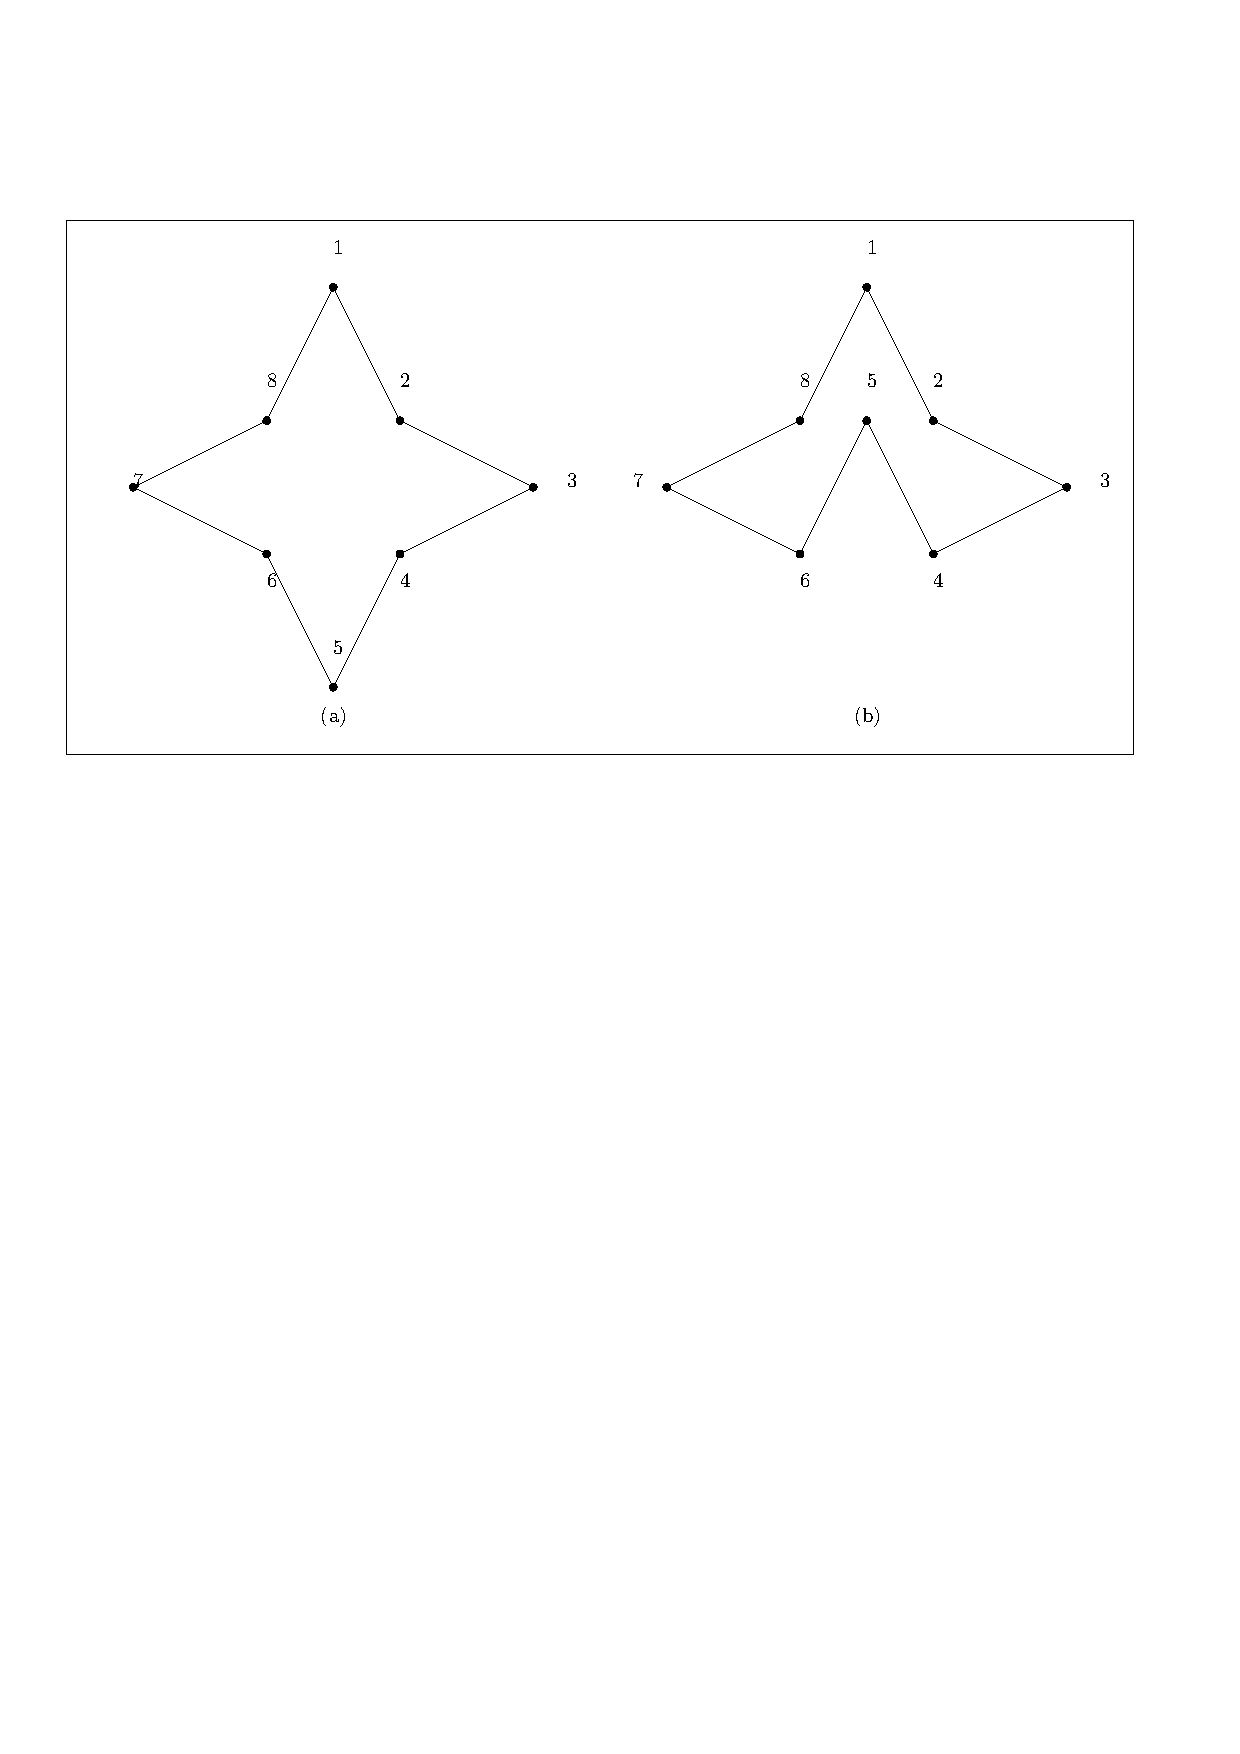
\includegraphics{graphics/twoEmbeddingsOfSameLinkage.pdf}
\end{center} 
\caption{(a) and (b) show a linkage in two embeddings.  Any realization of a path can be continuously moved without self-intersection to any other realizations.}
\label{fig:configuration-3}
\end{figure}

\subsection{Configuration Spaces of Polygonal Linkages}
The placement of a polygon is described by an isometry of Euclidian plane.
An isometry is a composition of a translation, a rotation, and a possible reflection.
As such, the isometry can be descibed as three parameters: $\lr{a,b,\theta}$ where $(a,b)$ is a translation vector; if $\theta \geq 0$, it describes a counter-clockwise rotation by $\theta$ and if $\theta < 0$, it descibes a reflection in the x-axis followed by a counter-clockwise rotation $\theta$.
For $m$ polygons there will be $3 m$ parameters.
Recall a realization of a polygonal linkage is an interior-disjoint placement of congruent copies of the polygons in $\PP$ such that the copies of a hinge are mapped to the same point (e.g., Figure \ref{fig:linkage-1}).
First consider the set of all realizations for the polygonal linkage $\left(\PP,\HH\right)$ and call it $P$.  
$\mu:P \mapsto \bbR^{3m}$ where $m$ is the number of polygons in $\PP$ is the configuration space function and the configuration space is the set $\mu(P)$. 

 \subsection{Configuration Spaces of Disk Arrangements}
rewrite where theta is not needed.  disks are symmetric and rotation does not help.
The placement of a polygon is described by an isometry of Euclidian plane.
An isometry is a composition of a translation, a rotation, and a possible reflection.
As such, the isometry can be descibed as three parameters: $\lr{a,b,\theta}$ where $(a,b)$ is a translation vector; if $\theta \geq 0$, it describes a counter-clockwise rotation by $\theta$ and if $\theta < 0$, it descibes a reflection in the x-axis followed by a counter-clockwise rotation $\theta$.
For $m$ polygons there will be $3 m$ parameters.
Recall a realization of a polygonal linkage is an interior-disjoint placement of congruent copies of the polygons in $\PP$ such that the copies of a contact are mapped to the same point (e.g., Figure \ref{fig:linkage-1}).
First consider the set of all realizations for the polygonal linkage $\left(\PP,\HH\right)$ and call it $P$.  
$\mu:P \mapsto \bbR^{3m}$ where $m$ is the number of polygons in $\PP$ is the configuration space function and the configuration space is the set $\mu(P)$. 

\begin{figure}[!htbp]
\begin{center}
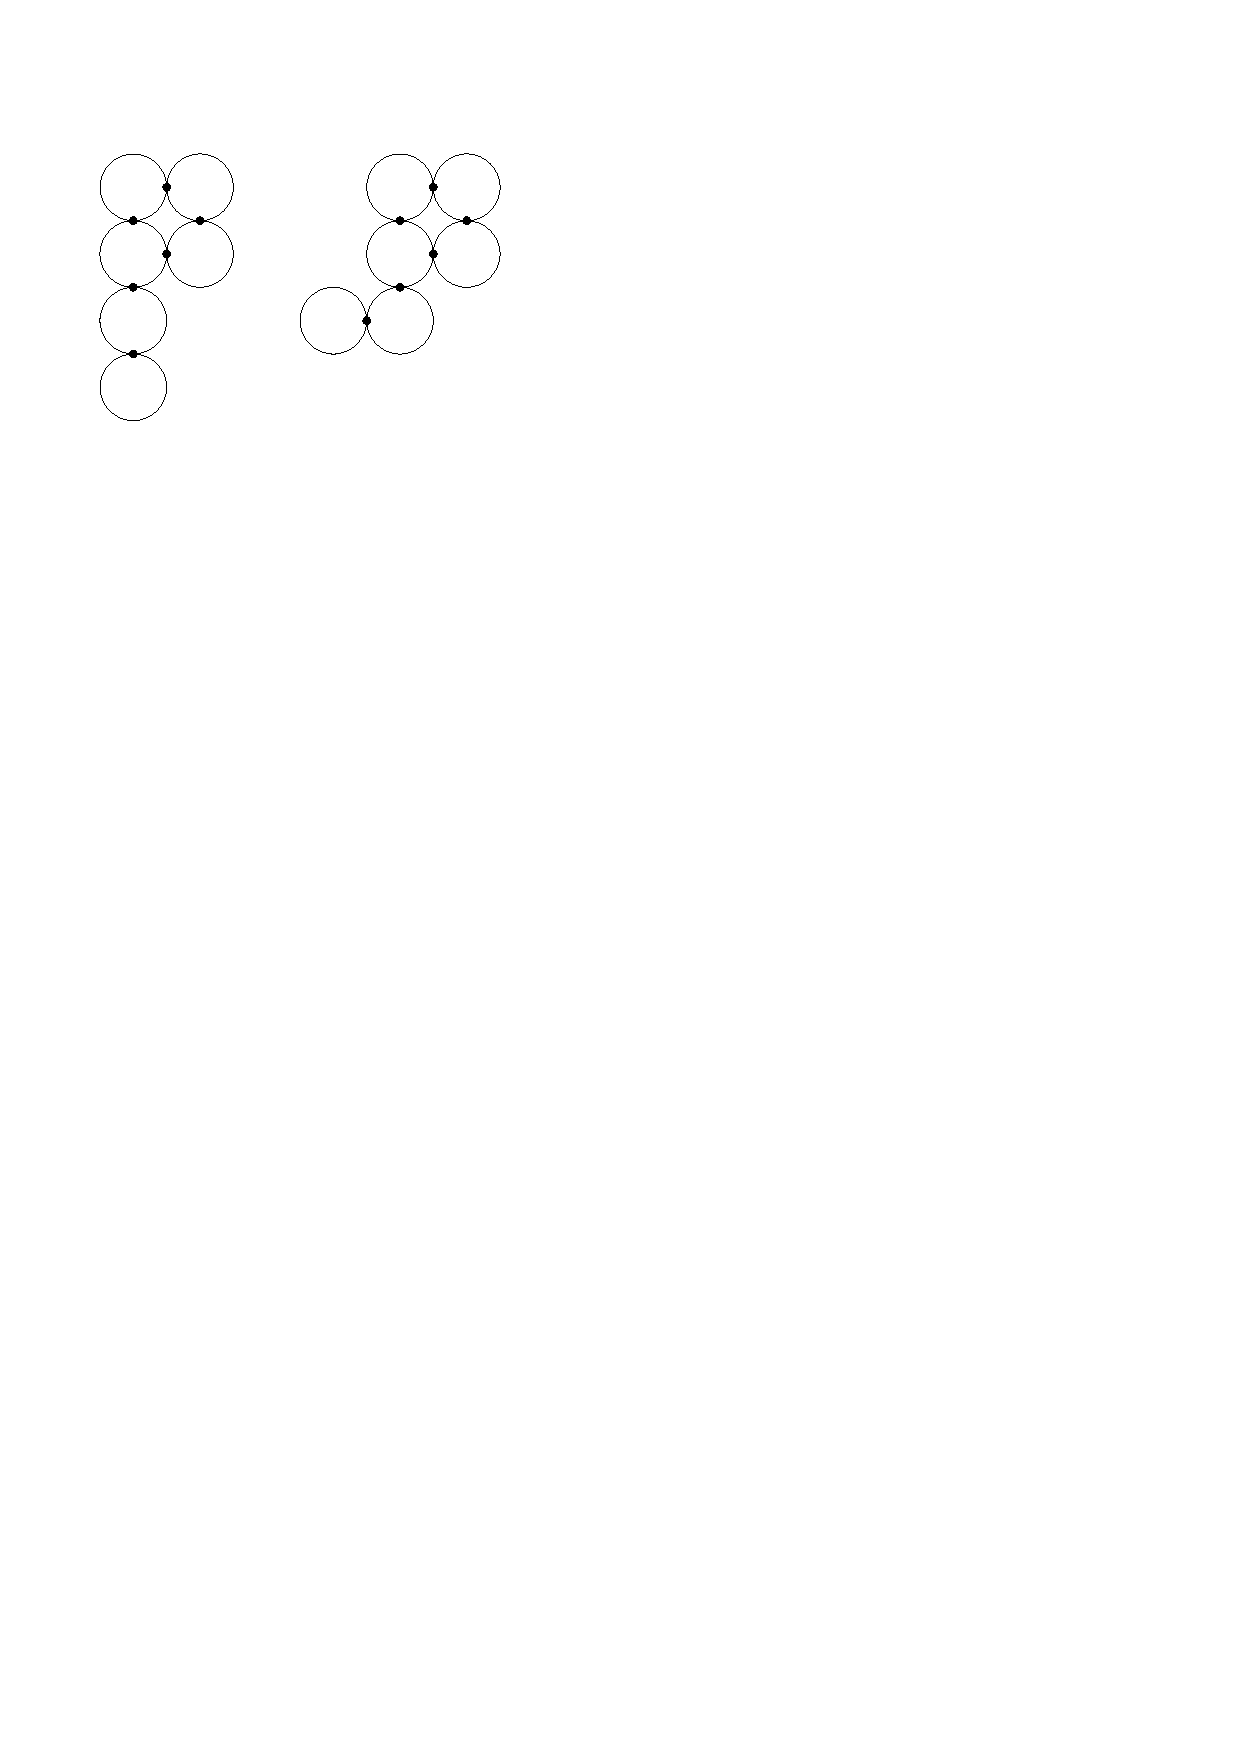
\includegraphics[scale=.75]{graphics/DiskPackingReconfiguration.pdf}
\end{center} 
\caption{An example of a disk arrangement where $A$ and $B$ have a large range of freedom to move around.  $C$, $D$, $E$, and $F$ are limited in their range of motion to due to their contact points.}
\label{fig:configuration-5}
\end{figure}

Consider the set of realizations $P$ for a given disk arrangement $\DD = \left\lbrace D_i \right\rbrace_{i=1}^n$.  For any realization $R \in P$, there exists a corresponding contact graph, $C$.  The configuration spaces of $\DD$ are sets of $R \in P$ that are classified by the equivalent contact graphs, i.e. if $R_1$, $R_2 \in P$ and their corresponding contact graphs $C_1$ and $C_2$ have a graph isomorphism, $\phi$, then $R_1$ and $R_2$ belong to the same configuration space.





% \subsection{Reconfiguration}



% We'd like to describe motions and range of motions of embedded graphs, linkages, polygonal 
% linkages, and disk arrangements.  Table \ref{table:configurationSpace-1} provides the definition of 
% \textit{reconfiguration} for each type of object covered so far:
% \begin{center}
% \begin{table}[htbp!]\label{table:configurationSpace-1}
% \begin{tabular}{|p{.2\textwidth}|p{.79\textwidth}|}
% \hline
% Object Type&Definition of Reconfiguration\\\hline
% Graph Embeddings&a continuous motion of the realized vertices that never causes the edges to 
% intersect.\\\hline
% Linkage&a continuous motion of the realized vertices that preserves the lengths of the edges and never 
% causes 
% the edges to intersect.\\\hline
% Polygonal Linkage&a continuous motion of polygons that preserves shapes of polygons, hinge point 
% pairings, and never causes the polygonal sides to intersect.\\\hline
% Disk Arrangement&a continuous motion of disks that preserves disk radii, pairs of contact points, 
% and never causes disks to intersect.\\\hline
% \end{tabular}
% \end{table}
% \end{center}








% 
% \paragraph{Confining Linkages to a Restricted Space Within a Configuration Space}
% So we've covered the idea of linkages within a plane; now let's constrain the plane to a strip and 
% have a linkage that is a \textit{polygon}, i.e. a linkage that forms a closed chain (e.g. Table 
% \ref{table:linkage-1}), hugging the boundaries of the strip:
% \begin{figure}[h]
% \begin{center}
%   ~ %add desired spacing between images, e. g. ~, \quad, \qquad etc.
%     %(or a blank line to force the subfigure onto a new line)
%   \begin{subfigure}[b]{0.49\textwidth}
% 	  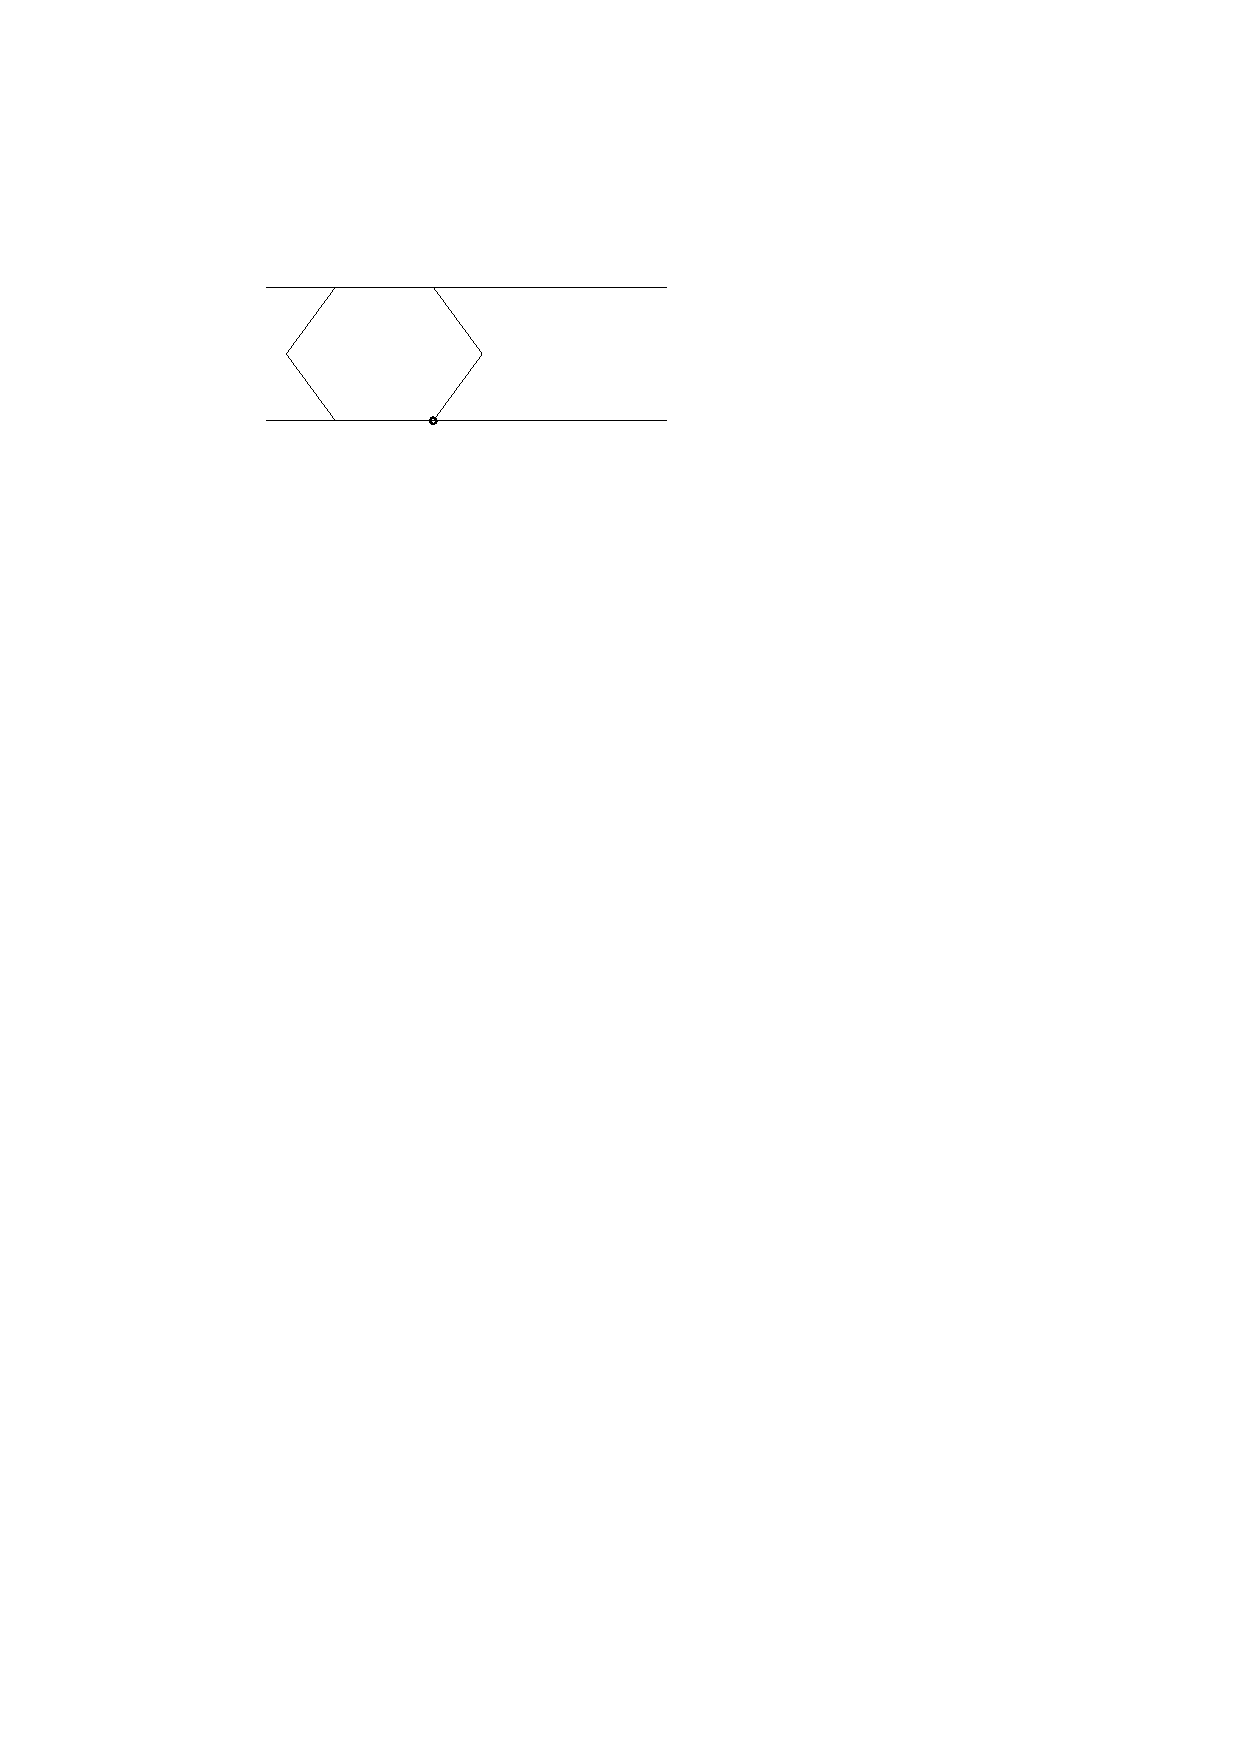
\includegraphics[width=\textwidth]{graphics/hexagonInChannelWithPinnedJointRight.pdf}
% 	  \caption{A bounded hexagon that resides in a channel with a pinned vertex}
% 	  \label{fig:linkage-1-1}
%   \end{subfigure}
%   \begin{subfigure}[b]{0.49\textwidth}
% 	  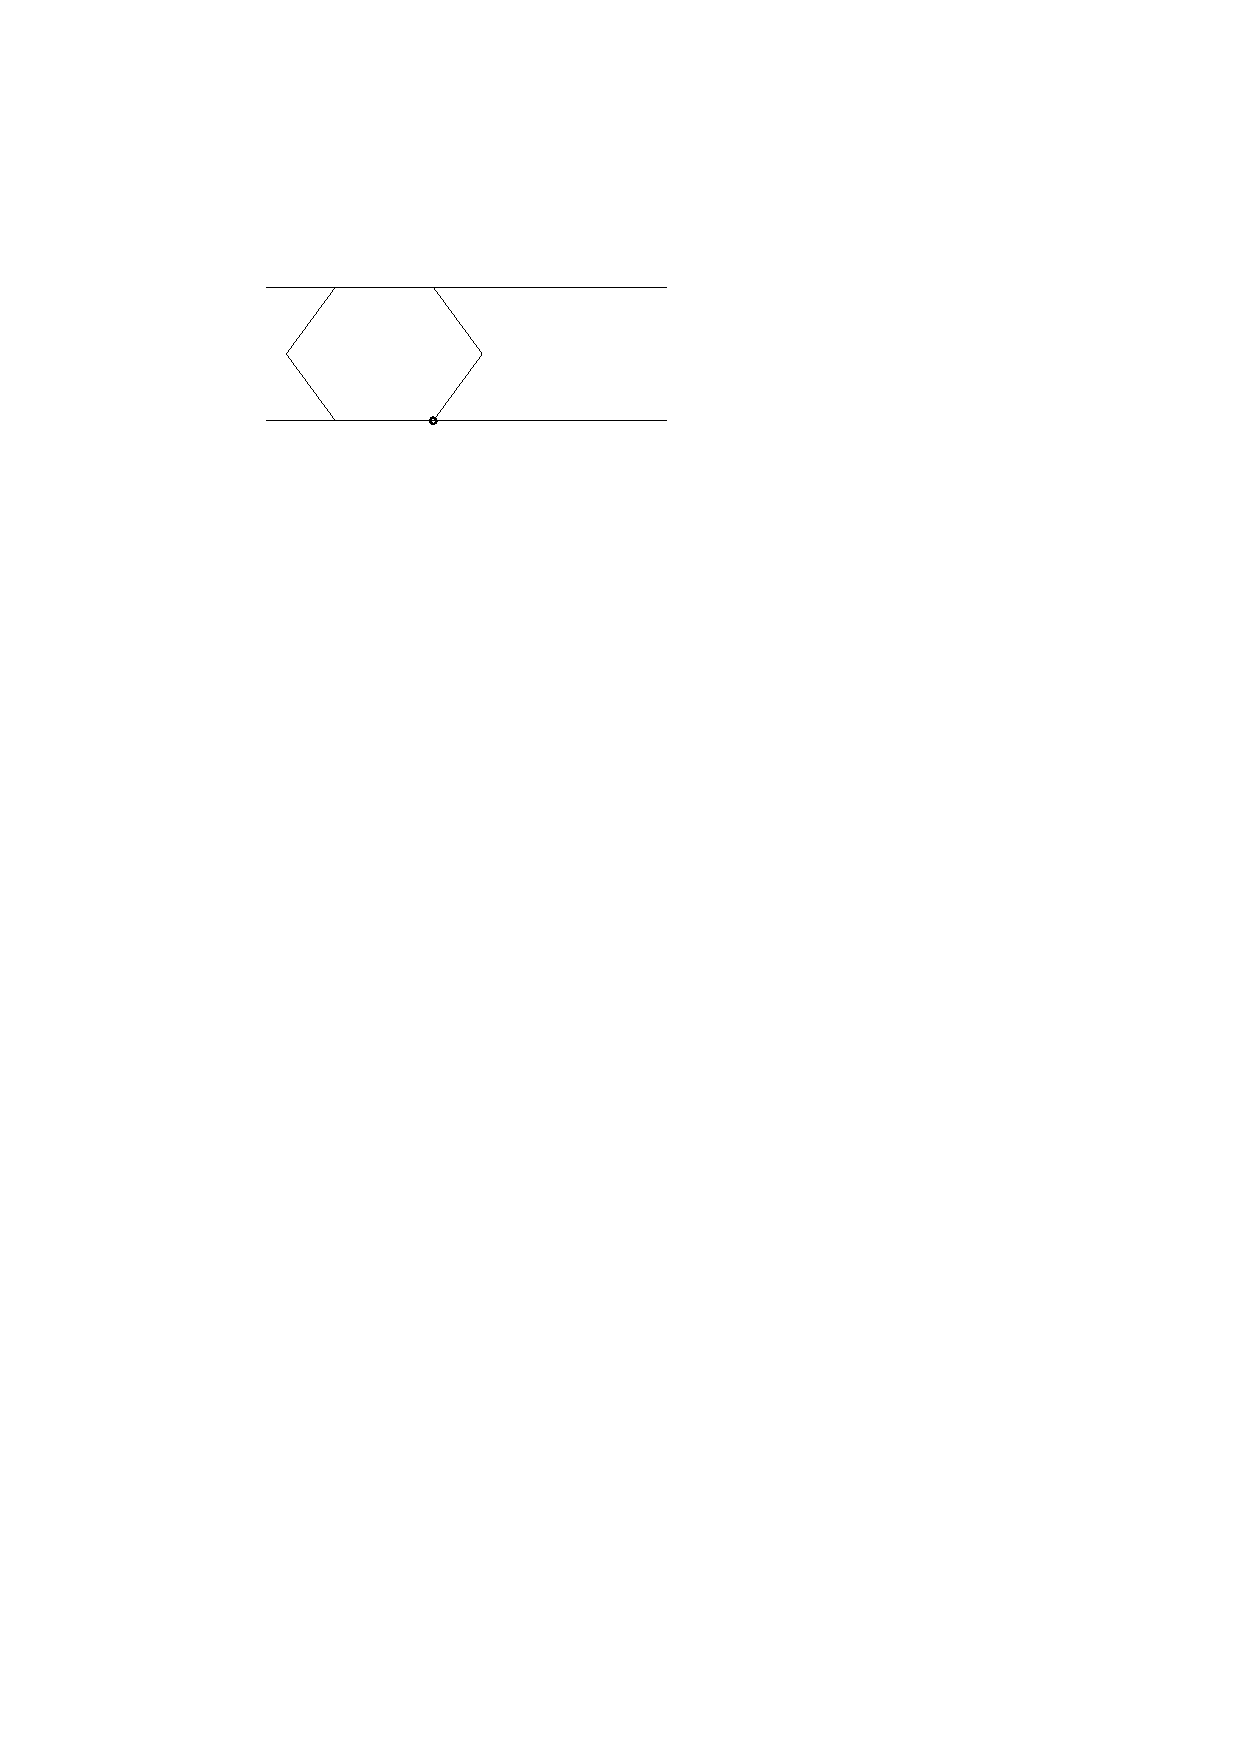
\includegraphics[width=\textwidth]{graphics/hexagonInChannelWithPinnedJointLeft.pdf}
% 	  \caption{The second realization of the hexagon residing in a channel with a pinned 
% vertex.}
% 	  \label{fig:linkage-1-2}
%   \end{subfigure}
% \end{center} 
% \caption{Due to the strip in the plane that the hexagon is bounded within the configuration space is 
% limited to just two realizations.}\label{fig:linkage-1}
% \end{figure}
% So here we have a linkage whose conifguration space is limited to just two realizations.  With just 
% two realizations, we can assign a binary value to them and have the linkage act as a boolean 
% variable.  We will revisit this concept when we cover satisfiability problems later on in the paper.
% \begin{figure}[h]
% \begin{center}
%   ~ %add desired spacing between images, e. g. ~, \quad, \qquad etc.
%     %(or a blank line to force the subfigure onto a new line)
%   \begin{subfigure}[b]{0.49\textwidth}
% 	  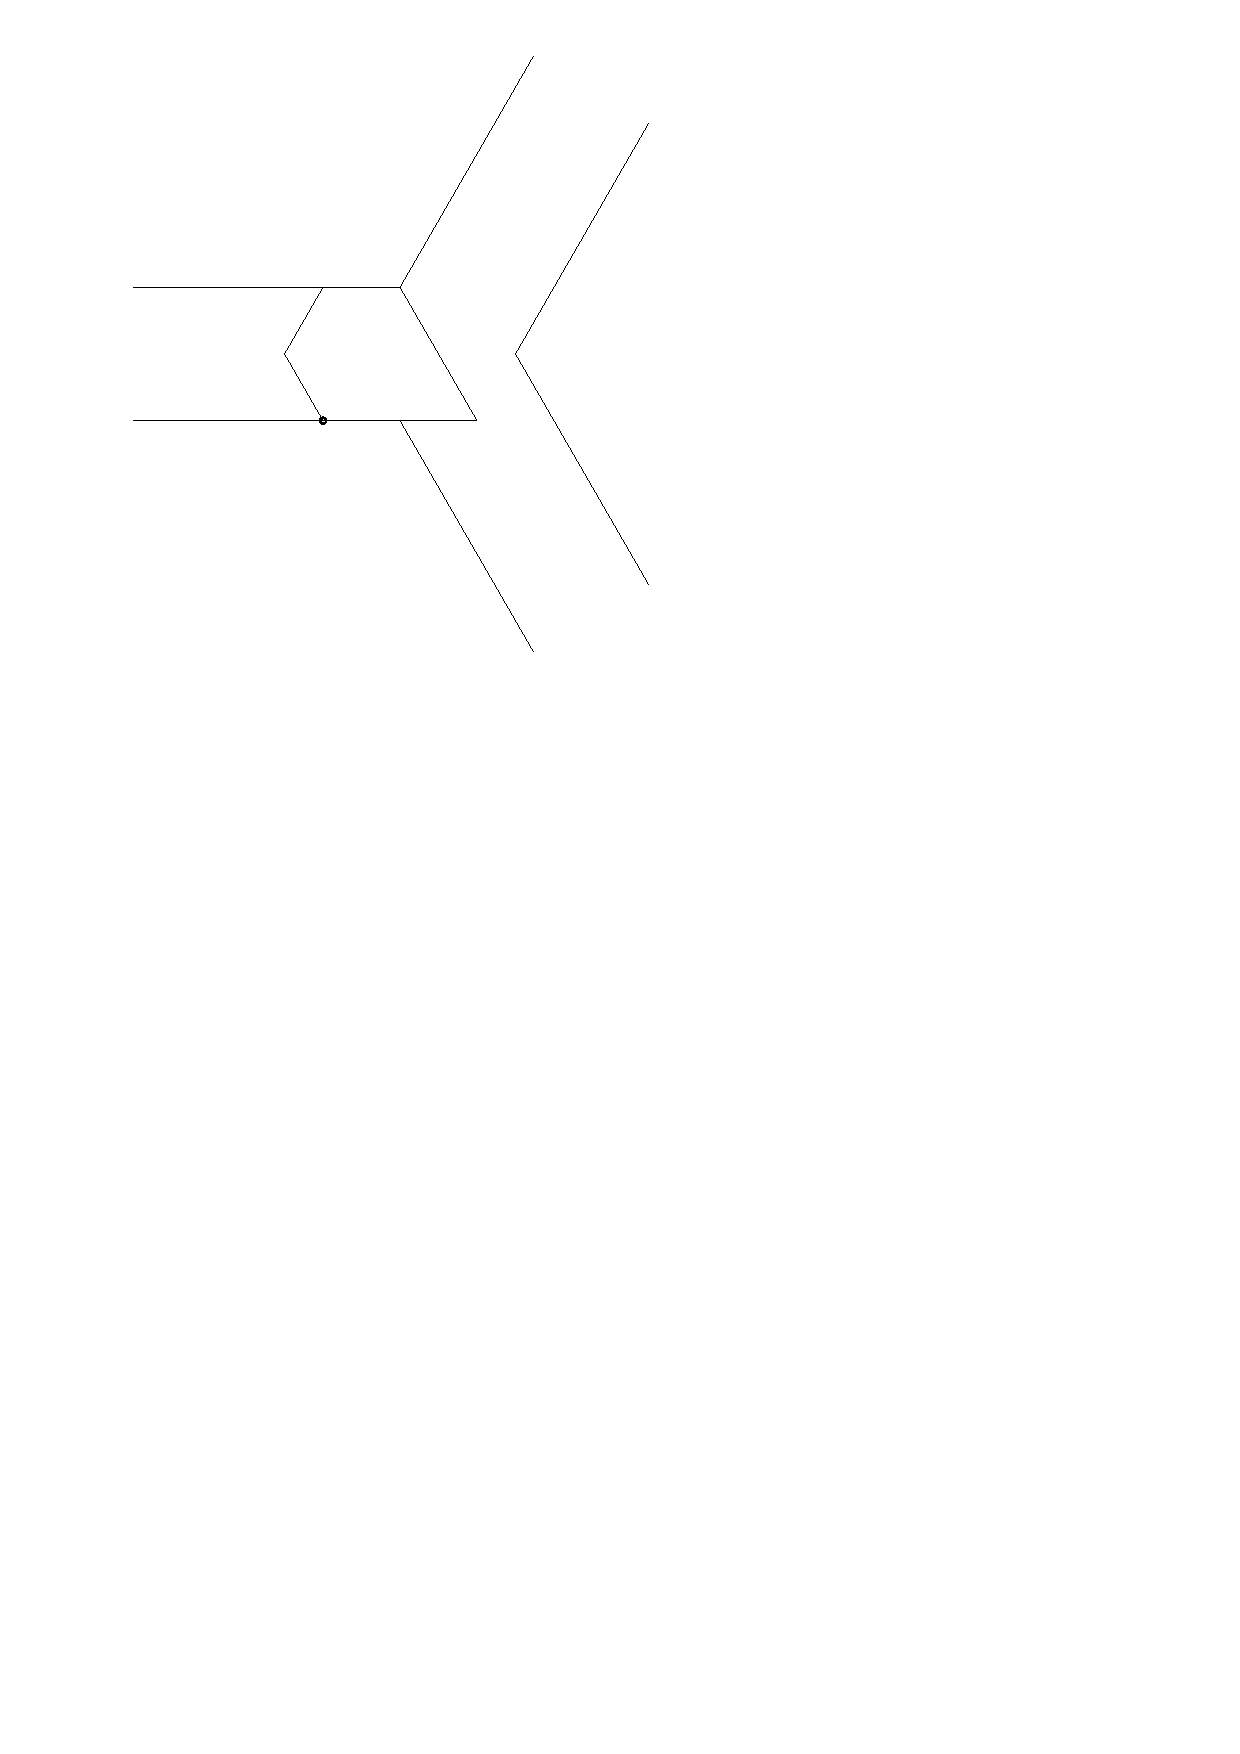
\includegraphics[width=\textwidth]{graphics/switchTerminalFinalized2.pdf}
% 	  \caption{A pentagon that is pinned in a channel junction that is formed by the sides of 3 
% large regular hexagons. It has two possible configurations, much like that of \ref{fig:linkage-1}}
% 	  \label{fig:linkage-2-1}
%   \end{subfigure}
%   \begin{subfigure}[b]{0.49\textwidth}
% 	  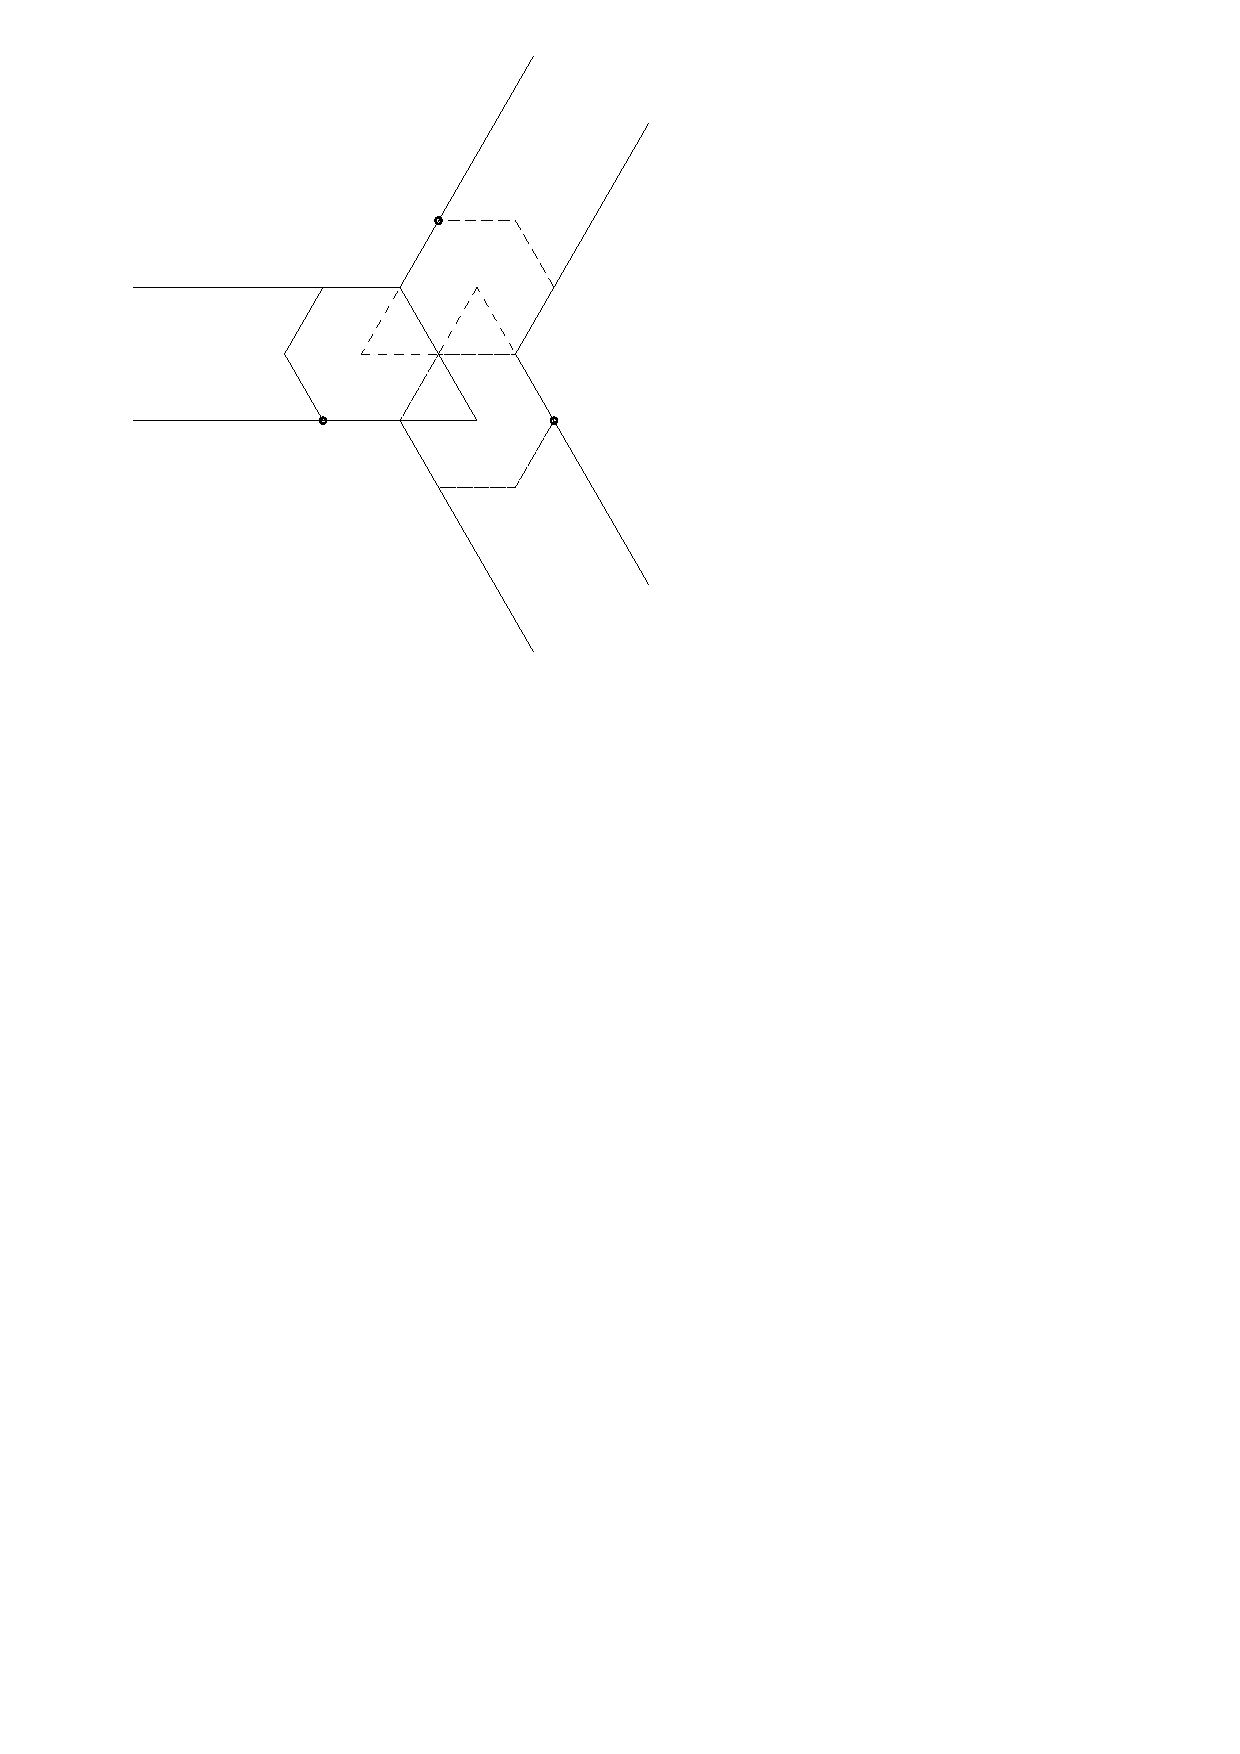
\includegraphics[width=\textwidth]{graphics/switchTerminalFinalized3.pdf}
% 	  \caption{A pinned pentagon residing in a channel junction that is formed by the sides of 
% 3 large regular hexagons with 2 dashed pentagons intersecting it.}
% 	  \label{fig:linkage-2-2}
%   \end{subfigure}
% \caption{Suppose the channel formed is a junction of three regular hexagons.  The polygon partially 
% residing in the junction is a regular hexagon with an equalateral triangle appended at an edge.  
% This polygon would prevent other polygons (i.e. the dashed polygons) of the same shape residing in 
% the center of the channel without intersection. This demonstrates that a the configuration space 
% within a multichannel environment can have concurrency issues, i.e. some configurations cannot be 
% realizable.}
% \end{center} \label{fig:linkage-2}
% \end{figure}\newpage
% Expanding upon the idea of \ref{fig:linkage-1}, forming channels with junctions as shown in Figure 
% \ref{fig:linkage-2} can be formed as such by evenly spacing the edges of a hexagonal lattice.  
% Visually, it is shown that only one of three possible pentagons can reside in the channel at one 
% time.  By asserting certain conditions on the lattice, and extending the problem to a greater 
% region 
% of a hexagonal lattice, we will be able to pose a realizability problem of whether a configuration 
% $\mathcal{A}$ can be reconfigured to $\mathcal{B}$ by switching pentagons without violating 
% overlapped polygon conditions.
% %Radius of regular polygons 
% %\newdimen\R
% %\R=3cm
% % \begin{figure}[h] 
% % \begin{center}
% % \begin{tikzpicture}
% % \begin{scope}
% % \filldraw[pattern=hexagons]  (0:\R) \foreach \x in {60,120,...,359} {
% %                 -- (\x:\R)
% %             }-- cycle (90:\R);
% % \end{scope}
% % \end{tikzpicture}
% % \caption{A hexagonal lattice contained in a hexagon.}
% % \label{fig:lattice}
% % \end{center}
% % \end{figure}
% %\newpage
% 
% % \begin{definition}[Graph]\label{def:linkages-2}
% % An ordered pair $G = (V, E)$ comprising a set $V$ of vertices or nodes together with a set $E$ of 
% edges or lines
% % \end{definition} 
% % \begin{definition}[Linkage]\label{def:linkages-1}
% % A collection of fixed-length 1D segments joined at their endpoints to form a graph.
% % \end{definition} 
% % A linkage can be thought of as a type of path-connected graph, i.e. the segments of a linkage are 
% the edges of a graph, and the endpoints of the segments are the vertices. For this paper, we 
% restrict our self to linkages that are simple planar graphs, i.e. a linkage that:
% % \begin{itemize}
% % \item[\rn{1}] does not have multiple edges between any pair of vertices,
% % \item[\rn{2}] does not have edges that cross, or
% % \item[\rn{3}] have loops (i.e. $(v,v) \in E$).
% % \end{itemize}  
% % \begin{definition}[Cycle]\label{def:linkages-3}
% %  A closed walk with no repetitions of vertices or edges allowed, other than the repetition of the 
% starting and ending vertex
% % \end{definition} 
% % \begin{definition}[Configuration]\label{def:linkages-6}
% % A specification of the location of all the link endpoints, link orientations and
% % joint angles.\cite{demaine2008geometric}
% % \end{definition}
% % \begin{definition}[Configuration Space]\label{def:linkages-7}
% % The space of all configurations of a linkage.
% % \end{definition} 
% % A configurations space is said to be continuous if for any two configurations, $\mathcal{A}$ and 
% $\mathcal{B}$ of a linkage $L$, $\mathcal{A}$ can be continuously reconfigured to $\mathcal{B}$ such 
% that, the reconfigurations reside in the configuration domain, $L$ remains rigid throughout 
% reconfiguration (i.e. all links' lengths are preserved), and no violations of linkage intersection 
% conditions. 
% % \begin{definition}[Pinned Joint]\label{def:linkages-8}
% % A vertex of a graph (or linkage) that is fixed to a position in a plane.
% % \end{definition} 
% % \begin{definition}[Free Joint]\label{def:linkages-8}
% % A vertex of a graph (or linkage) that is not fixed to a position in a plane.
% % \end{definition} x
% % \begin{figure}[h]
% % \begin{center}
% % 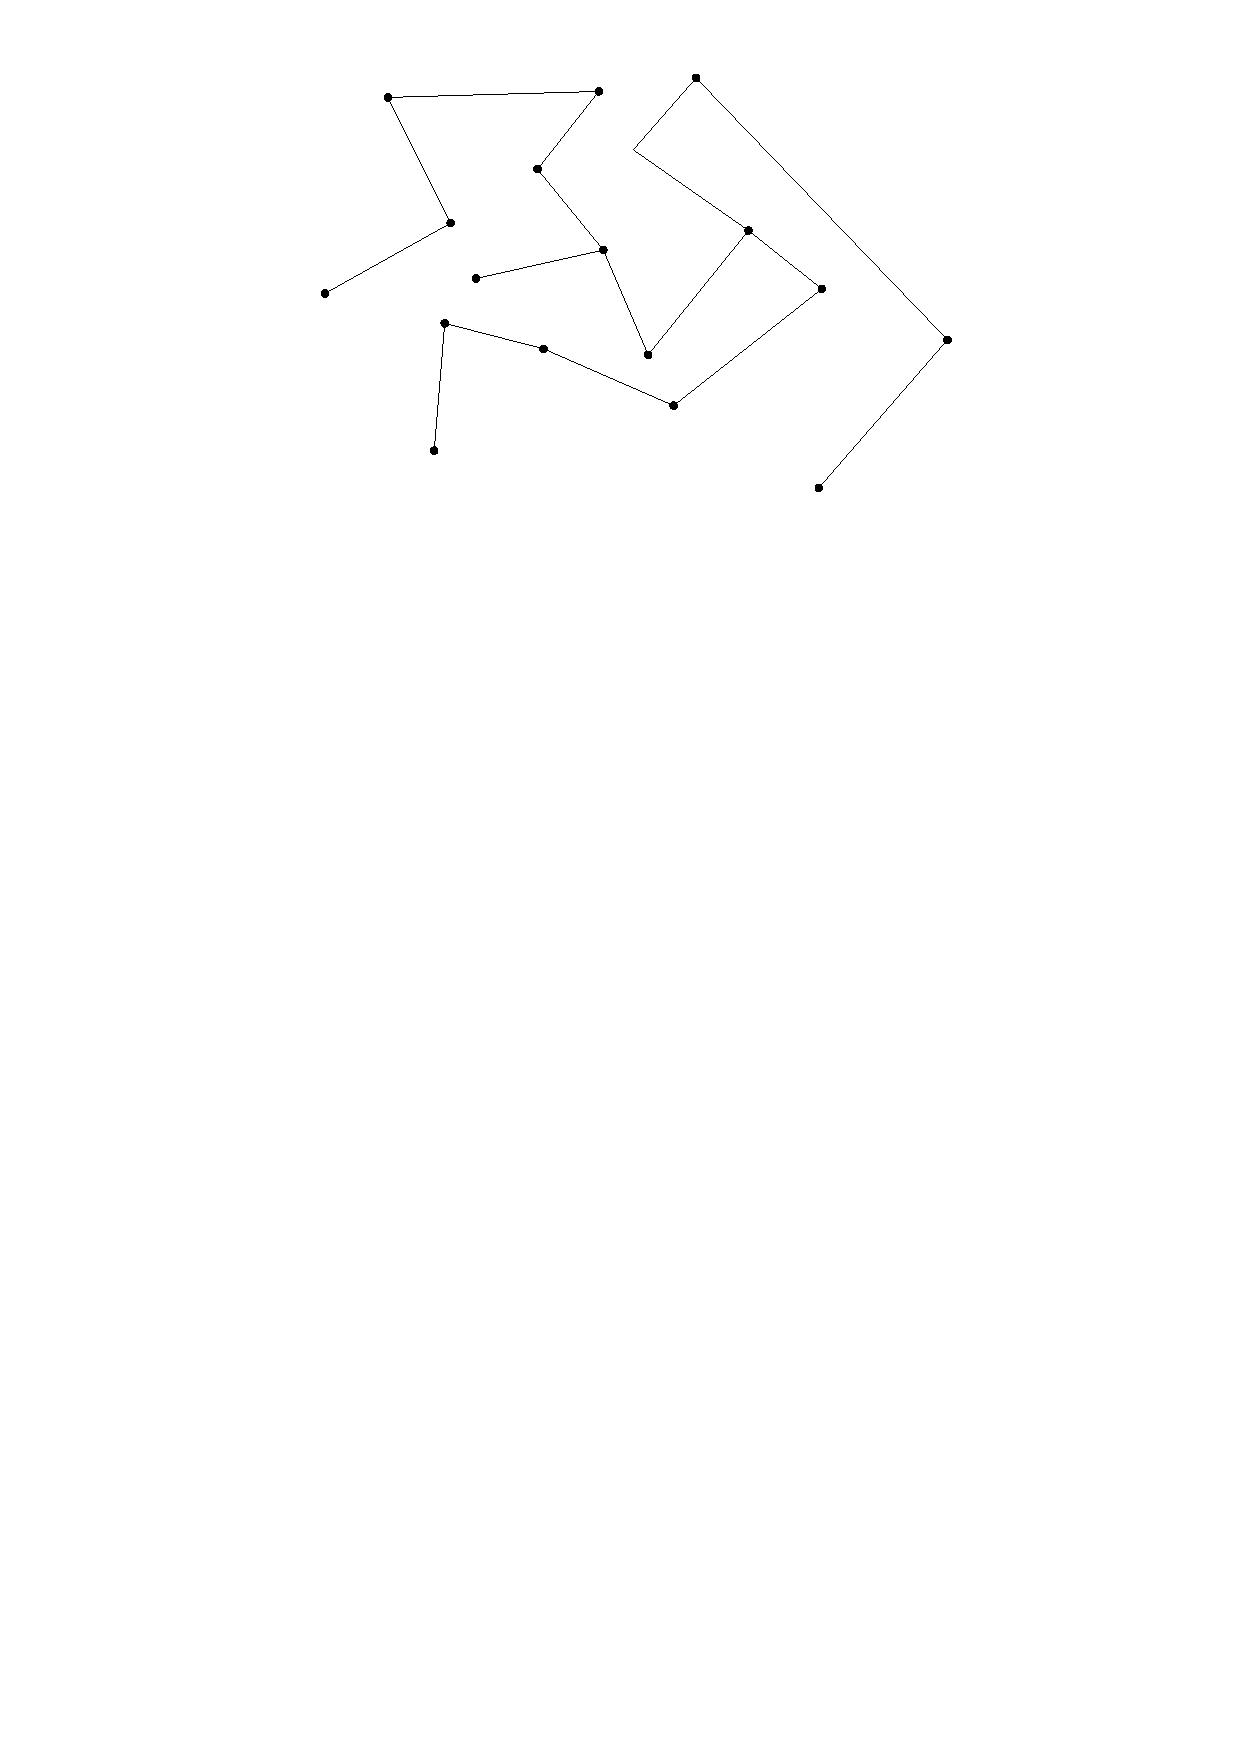
\includegraphics[scale=.5]{graphics/randomLinkage.pdf}
% % \end{center} 
% % \caption{A linkage with joints.}
% % \end{figure} 
% % \begin{figure}[h]
% % \begin{center}
% % 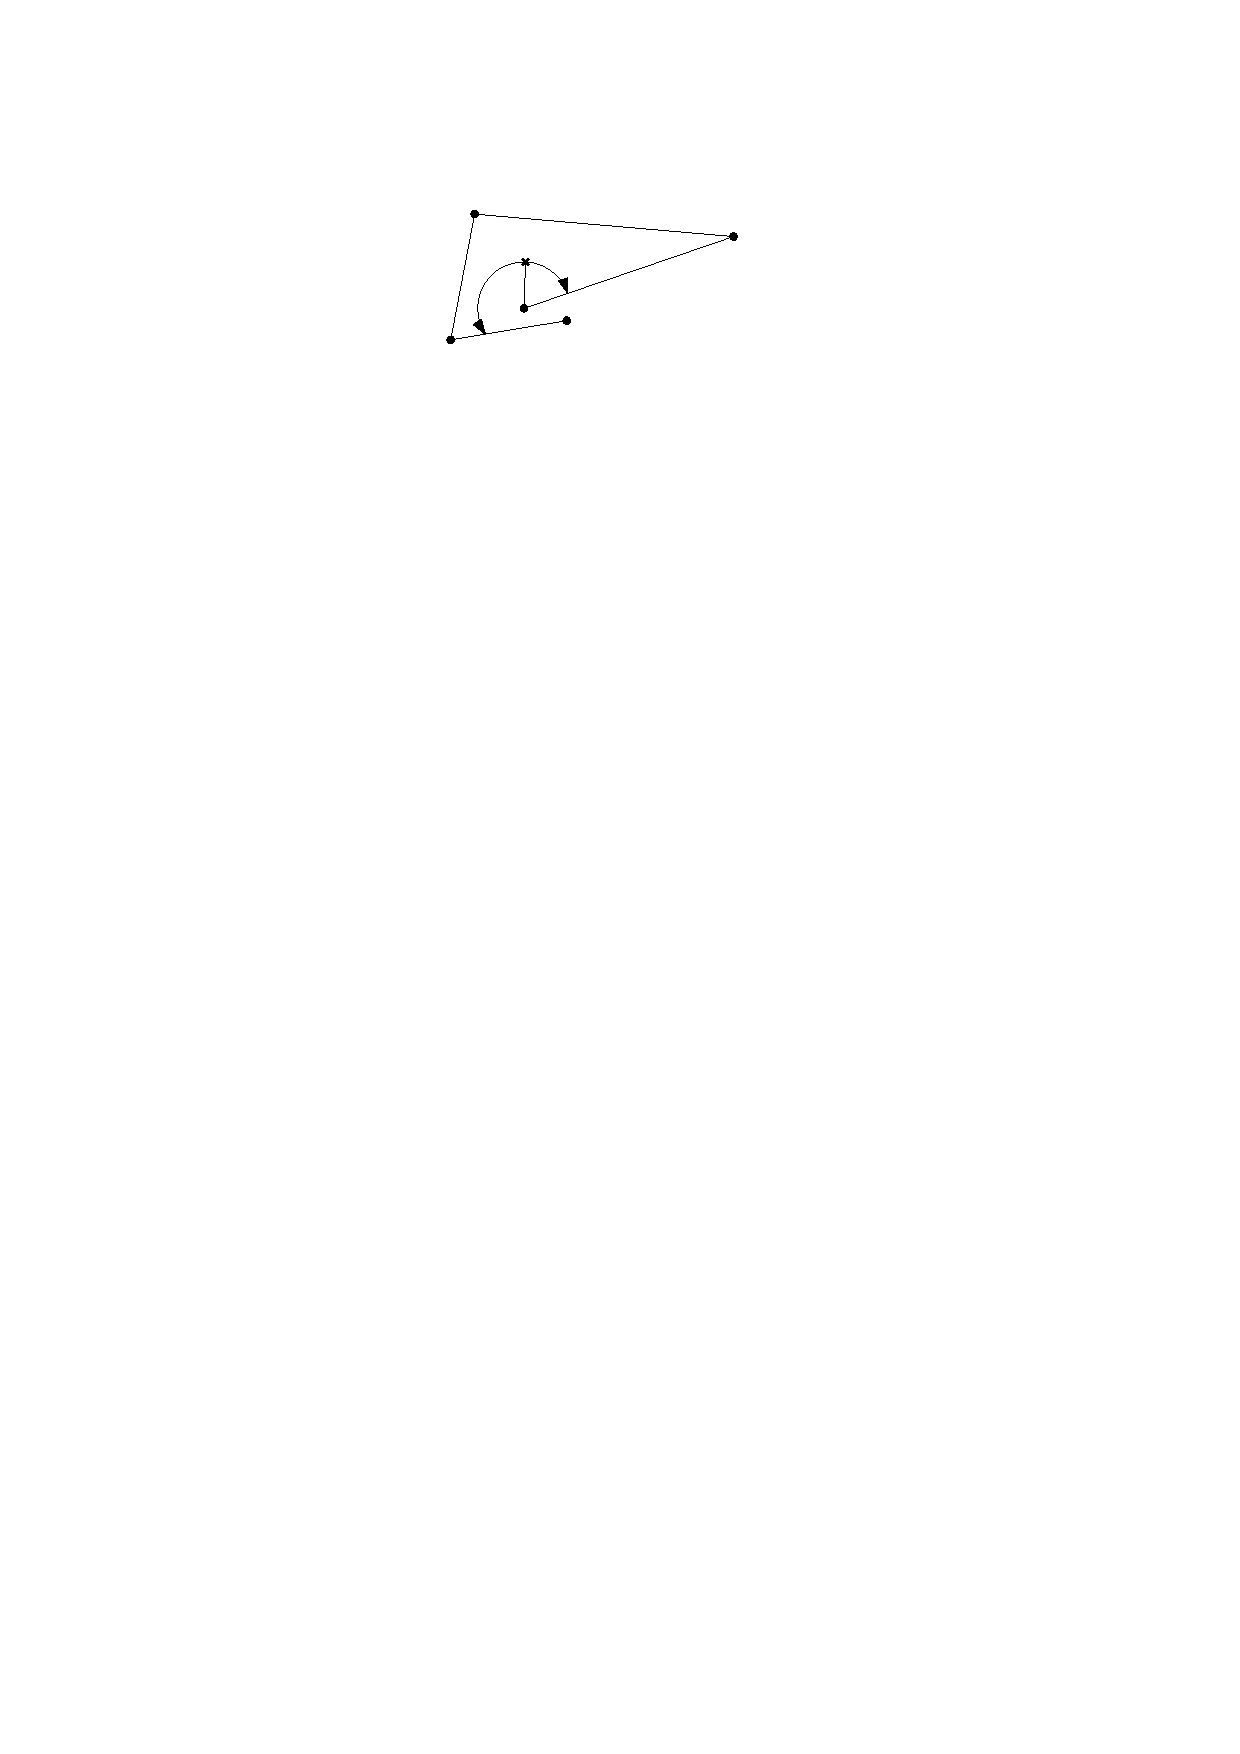
\includegraphics{graphics/freeJointPinnedJoint.pdf}
% % \end{center} 
% % \caption{The cross represents a free joint; the pinned joints are denoted as disks.  The range of 
% motion shown by the arc describes the continous configuration space of the linkage.}
% % \end{figure} 
% % 
% % For illustrations in the remainder of this paper, free joints will be represented as crosses and 
% pinned joints will be represented as disks.

%I) Algorithm Complexity
%	a) Algorithm
%		procedure of calculations
%		has a running time
%		utilizes resources
%		goal: have an algorithm that runs quickly and utilizes a small amount of resources
%	b) Qualitative Analysis of Algorithms
%		worst case running time
%		brute force
%		efficiency
%	c) Spaces of Algorithms
%		polynomial time
%		PSPACE
%		NP
%		P
%		NP-Complete
\section{Algorithm Complexity}
\textit{Algorithms} are a set of procedural calculations.  When an algorithm executes its procedure it can be measured in terms of units of consumed resources (in computers, that is memory) and the time it takes to complete the procedure of calculations.  Ideally, a desirable algorithm would run quickly and utilizes a small amount of resources.

\subsection{Qualitative Analysis of Algorithms  
etermining the time and space that algorithms use determine their efficiency.  The \textit{worst-case} running time is the largest possible running time that an algorithm could have over all inputs of a given size $N$.  \textit{Brute force} is when an algorithm tries all possibilities to see if any formulates a solution.  An algorithm is said to be \textit{efficient} if it achieves qualitatively better worst-case performance, at an analytical level, than brute force search \cite{kleinberg2006algorithm}.


\subsection{Categorization of Algorithms}
For combinatorial problems, as the number of inputs of the problem grows, the solution space tends to grow exponentially.  In general, as problems grow, it is desirable to minimize the \textit{running time}, time take to run an algorithm that solves a problem. There are various types of running times; the running time that we will focus on in this thesis is polynomial running time.  \textit{Polynomial running time} is if the input size increases from $N$ to $2\cdot N$, the bound on the running time increases from $c \cdot (2N)^d = c \cdot 2^d \cdot N^d$.  

To categorize problems \cite{kleinberg2006algorithm}, we ask the following:
\begin{prob}
Can arbitrary instances of problem $Y$ by solved using a polynomial number of standard computational steps, plus a polynomial number of calls to an algorithm that solves $X$?
\end{prob}
The class of problems that can be solved in polynomial running time is called the \textit{polynomial time} class.  

\section{Satisfiability}
\begin{prob}[Satisfiability Problem]\label{prob:Satisfiability-1}%Problem/Question
Let $\left\lbrace x_i \right\rbrace_{i=1}^{n} $ be boolean variables, and $t_i \in \left\lbrace 
x_i\right\rbrace_{i=1}^{n}  \cup \left\lbrace \bar{x}_i\right\rbrace_{i=1}^{n}   $.  A 
\textit{clause} is is said to be a disjuction of distinct terms:
$$
t_1 \vee \cdots \vee t_{j_k} = C_k
$$
Then the \textit{satisfiability problem} is the decidability of a conjuction of a set of clauses, 
i.e.:
$$ \wedge_{i=1}^m C_i$$
\end{prob} \cite{skiena2009algorithm}
A \textit{3-SAT problem} is a SAT problem with all clauses having only three boolean variables. 
\begin{definition}[Planar 3-SAT Problem]\label{def:Satisfiability-2}
Given a boolean 3-SAT formula $B$, define the associated graph of $B$ as follows:  
\begin{equation}\label{eqn:sat-1}
G(B) = \left(\set{v_x}{v_x\text{ represents a variable in }B} \cup \set{v_C}{v_C\text{ represent a 
clause in }B}  , \set{\left( v_x, v_C\right) }{x \in C \text{ or } \bar{x} \in C}  \right) 
\end{equation} 
If $G(B)$ in equation (\ref{eqn:sat-1}) is planar, then $B$ is said to be a \textit{Planar 3-SAT 
Problem} \cite{mulzer2008minimum}.
\end{definition}
\subsection{Not All Equal 3 SAT Problem}
\begin{prob}[Not All Equal 3 SAT Problem]\label{prob:Satisfiability-2}%Problem/Question
Give a set of clauses $C$, each containing three boolean variables, can each clause contain at 
least one true variable and one false variable?
\end{prob}
\subsection{Planar 3 SAT Problem}
% Definition 1. (PLANAR 3-SAT) Let Φ be a
% Boolean formula in 3-CNF. The formula graph of
% Φ, G(Φ), has one variable-vertex vx for each variable
% x and one clause-vertex vC for each clause C. The
% variable-vertices vx are connected by edges to form a
% variable cycle, and for each clause-vertex vC an edge
% (vC, vx) is added if C contains either literal x or x.
% We say Φ is planar iff G(Φ) is planar. The PLANAR
% 3-SAT problem is equivalent to the 3-SAT problem
% restricted to planar formulae.
% Theorem 2.1. (Lichtenstein [14] Theorem 2)
% PLANAR 3-SAT is NP-complete
\begin{prob}[Planar 3 SAT Problem]
 A planar 3SAT instance is a 3SAT instance for which the graph built using the following rules is 
planar:
\begin{enumerate}
 \item add a vertex for every $x_i$ and $\bar{x}_i$
 \item add a vertex for every clause $C_j$
 \item add an edge for every $\left(x_i,\bar{x}_i \right)$ pair
 \item add an edge from vertex $x_i$ (or $\bar{x}_i$) to each vertex that represent a clause that 
contains it
 \item add edges between two consecutive variables $(x_1,x_2)$, $(x_2,x_3)$, $\dots$,$(x_n,x_1)$
\end{enumerate}
In particular, rule 5 builds a "backbone" that splits the clauses in two distinct regions.
\end{prob}

%Universality component
\subsection{Logic Engine}
The logic engine simulates the well known Not All Equal 3 SAT Problem (NAE3SAT).  
%add figure of logic engine.
\subsection{Construction of the Logic Engine}
The components of the logic engine are as follows: the rigid frame, the shaft, the armatures, 
the chains, and the flags.  The \textit{rigid frame} is a rectangular enclosure with a horizontal 
shaft place at mid-height.  The \textit{armatures} are concentric rectangular frames contained 
within the rigid frame.  Each armature can rotate about the shaft; other motions on the armature 
are disallowed.  Given an NAE3SAT, for each variable there is a corresponding armature. On each 
armature, there are chains.  A pair of \textit{chains}, $a_j$ and $\bar{a}_j$ correspond to the 
variable $x_j$ and $\bar{x}_j$ respectively.  The pair is placed on each armature, reflected at a 
height of $h$ above and below the shaft, i.e. one place above the shave at a height of $h$, the 
other placed below the shaft at a height of $-h$.
%insert an armature graphic

\subsection{Encoding the Logic Engine}
For each clause of an NAE3SAT, there exists a set of corresponding chains, namely the $h^\text{th}$ 
clause is the set of chains on the armatures at the $h^\text{th}$ row above and below the shaft. A 
chain is \textit{flagged} if the corresponding variable resides within the clause.  The flag can 
point in either the left or right directions indicating a truth assignment for that variable within 
the clause.  A flag is attached to the $i^\text{th}$ chain of every $a_j^\text{th}$ and 
$\bar{a}_j^\text{th}$ chain with the following exceptions:
\begin{enumerate}
 \item if the variable $x_j$  is in clause $C_i$, then link $i$ of $a_j$ is unflagged,
 \item if the variable $\bar{x}_j$ is in clause $C_i$, then link $i$ of $a_j$ is unflagged.
\end{enumerate}
\begin{thm}\label{thm:Satisfiability-1}
 An instance of $NAE3SAT$ is a ``yes'' instance if and only if the corresponding logic engine has a 
flat, collision-free configuration.
\end{thm}
\begin{pf}
 If an instance of $NAE3SAT$ is a ``yes'', then every clause in $C$ contains at least one true 
variable and one false variable.  Now suppose the following truth assignment:
\begin{equation}\label{eqn:Satisfiability-1}
 t\left( x_j \right) = \left\lbrace\begin{array}{cr}
  1 & x_j\text{ and }\bar{x}_j \text{are placed at the top and bottom respectively}\\
  0 & x_j\text{ and }\bar{x}_j \text{are placed at the bottom and top respectively}\\
 \end{array}\right.
\end{equation}
For each clause $c_i \in C$, there exists a variables in $c_i$ such that $t\left( y_i \right) = 1$ 
and $t\left( z_i \right) = 0$.  This implies that there exists an unflagged chain in the 
$i^\text{th}$ and $-i^\text{th}$ row of the frame.  To avoid a collision in each row, trigger the 
flags to point towards the unflagged link. Thus, the corresponding logic engine has a 
flat, collision-free configuration.

If the corresponding logic engine has a flat, collision-free configuration, then there must exist 
an unflagged link in each row.  Without loss of generality, we have that the variables $y_j$ and 
$z_i$ is in clause $C_i$ such that $t\left( y_i \right) = 1$ and $t\left( z_i \right) = 0$ for each 
$i$.  Thus, we have an instance of $NAE3SAT$ is a ``yes'' instance. \cite{BET+99}
\end{pf}


\section{Contribution}
The \emph{realizability} problem for a polygonal linkage asks whether a given polygonal linkage has 
a realization (resp., orientated realization). For a weighted planar (resp., plane) graph,, it asks 
whether the graph is
the contact graph (resp., ordered contact graph) of some disk arrangement with specified radii. 
These problems, in general, are known to be NP-hard. Specifically, it is NP-hard to decide whether a 
given planar (or plane) graph can be embedded in $\RR^2$ with given edge lengths~\cite{CDD+10,EW90}. 
Since an edge of given length can be modeled by a suitably long and skinny rhombus, the 
realizability of polygonal linkages is also NP-hard. The recognition of the contact graphs of unit 
disks in the plane (a.k.a. coin graphs) is NP-hard~\cite{BK98}, and so the realizability of weighted 
graphs as contact graphs of disks is also NP-hard. However, previous reductions crucially rely on 
configurations with high genus: the planar graphs in~\cite{CDD+10,EW90} and the coin graphs 
in~\cite{BK98} have many cycles.

In this thesis, we consider the above four realizability problems when the union of the polygons 
(resp., disks) in the desired configuration is simply connected (i.e., contractible). That is, the 
contact graph of the disks is a tree, or the ``hinge graph'' of the polygonal linkage is a tree (the 
vertices in the \emph{hinge graph} are the polygons in $\PP$, and edges represent a hinge between 
two polygons). Our main result is that realizability remains NP-hard when restricted to simply 
connected structures.
 
 % \subsection{Problem Statement} 
%write up thm 1, 2 (unoriented versions of the problem)
%write up thm 3, 4 (oriented versions of the problem)
\begin{thm}\label{thm:hinge2}
It is strongly NP-hard to decide whether a polygonal linkage whose hinge graph is a \textbf{tree} can be realized.
\end{thm}
\begin{thm}\label{thm:hinge3}
It is strongly NP-hard to decide whether a polygonal linkage whose hinge graph is a \textbf{tree} can be realized with fixed orientation.
\end{thm}
Our proof for Theorem \ref{thm:hinge3} is a reduction from {\sc Planar-3-SAT} (P3SAT): decide whether a given Boolean formula in 3-CNF with a planar associated graph is satisfiable. 
Our proof for Theorem \ref{thm:hinge2} is a reduction from {\sc Not-All-Equal-3-SAT} (NAE3SAT): decide whether a given Boolean formula in 3-CNF  is it satisfiable so that each clause contains a true and a false literal?


\begin{thm}\label{thm:hinge}
It is NP-Hard to decide whether a polygonal linkage whose hinge graph is a tree can be realized 
(both with and without orientation).
\end{thm}

\begin{thm}\label{thm:disk}
It is NP-Hard to decide whether a given tree (resp., plane tree) with positive vertex weights
is the contact graph (resp., contact graph) of a disk arrangements with specified radii.
\end{thm}

The unoriented versions, where the underlying graph (hinge graph or contact graph) is a tree can 
easily be handled with the logic engine method (Section~\ref{sec:logic}). We prove 
Theorem~\ref{thm:hinge} for \emph{oriented} realizations with a reduction from {\sc Planar-3SAT} 
(Section~\ref{sec:hinge}), and then reduce the realizability of ordered contact trees to the 
oriented realization of polygonal linkages by simulating polygons with arrangements of disks 
(Section~\ref{sec:disk}).


% \subsection{Decidability of Problem} test
% \subsection{Hexagonal Locked Configuration}
%write up thm 1, 2 (unoriented versions of the problem)
%write up thm 3, 4 (oriented versions of the problem)
\begin{prob}[Unordered Realizibility Problem for Linkages]
For a linkage, it asks 
whether its corresponding graph is the contact graph (resp., ordered contact graph) of some disk 
arrangement with specified radii.
\end{prob}
\begin{prob}[Unordered Realizibility Problem for Polygonal Linkages]
The \emph{realizability} problem for a polygonal linkage asks whether a given polygonal linkage has 
a realization.
\end{prob}
\begin{prob}[Ordered Realizibility Problem for Linkages]
For a linkage, it asks 
whether its corresponding graph is the ordered contact graph of some 
disk arrangement with specified radii.
\end{prob}
\begin{prob}[Ordered Realizibility Problem for Polygonal Linkages]
The \emph{realizability} problem for a ordered polygonal linkage asks whether a given polygonal 
linkage has a realization with respect to order.
\end{prob}



\end{document}
